\documentclass{article}
\usepackage[margin=1.5in]{geometry}

%%%% PACKAGES TO USE
\usepackage[utf8]{inputenc} % allow utf-8 input
\usepackage[T1]{fontenc}    % use 8-bit T1 fonts
\usepackage{hyperref}       % hyperlinks
\usepackage{url}            % simple URL typesetting
\usepackage{booktabs}       % professional-quality tables
\usepackage{amsfonts}       % blackboard math symbols
\usepackage{nicefrac}       % compact symbols for 1/2, etc.
\usepackage{microtype}      % microtypography

% Math related
\usepackage{amsmath}
% Indicator
%\usepackage{bbm} %uses Type3
\usepackage{dsfont} %works with Type1
% Figures and subfigures
\usepackage{graphicx}
\usepackage{caption}
\usepackage{subcaption}
\usepackage{float} %Stay where told
% Tables
\usepackage{booktabs} % for professional tables
\usepackage{multirow} % to be able to have multiple row expanding cell
\usepackage[table]{xcolor}
% Reference column balancing
\usepackage{flushend}
% Algorithms
\usepackage{algorithm}
\usepackage{algorithmic}
% To draw graphs
\usepackage{tikz}
\usetikzlibrary{bayesnet} % Library for bayesian networks

% Bibliography
\usepackage[round,numbers,sort]{natbib}

%%%% DEFINITIONS-MACROS
% Real line
\def \Real{{\mathbb R}} 
\def \Natural{{\mathbb N}} 
%Expected value
\newcommand{\eValue}[1]{\mathbb{E}\left\{ #1 \right\}}
% My small matrix
\newcommand{\mySmallMatrix}[1]{\left(\begin{smallmatrix} #1 \end{smallmatrix}\right)}
%Determinant
\newcommand{\mydet}[1]{\left| #1 \right|}
\newcommand{\HH}{\mathcal{H}}

% Abbreviations
\newcommand{\iid}{i.i.d. }
\newcommand{\ie}{i.e., }
\newcommand{\Ie}{I.e., }
\newcommand{\eg}{e.g., }
\newcommand{\Eg}{E.g., }
\newcommand{\etAl}{et al.\xspace}

%Distributions
\newcommand{\N}[1]{\mathcal{N}\left( #1\right)}
\newcommand{\MN}[1]{\mathcal{MN}\left( #1\right)}
\newcommand{\T}[1]{\mathcal{T}\left( #1\right)}
\newcommand{\MT}[1]{\mathcal{MT}\left( #1\right)}
\newcommand{\Dir}[1]{{\rm Dir\left( #1\right)}}
\newcommand{\Mult}[1]{{\rm Mult}\left( #1\right)}
\newcommand{\Cat}[1]{{\rm Cat}\left( #1\right)}
\newcommand{\Bin}[1]{{\rm Bin}\left( #1\right)}
\newcommand{\IG}[1]{{\rm IG}\left( #1\right)}
\newcommand{\NIG}[1]{{\rm NIG}\left( #1\right)}
\newcommand{\NIX}[1]{{\rm NIX}\left( #1\right)}
\newcommand{\IW}[1]{{\rm IW}\left( #1\right)}
\newcommand{\NIW}[1]{{\rm NIW}\left( #1\right)}
\newcommand{\Beta}[1]{{\rm Beta}\left( #1\right)}
\newcommand{\Ber}[1]{{\rm Ber}\left( #1\right)}
\newcommand{\U}[1]{\mathcal{U}\left( #1\right)}

%Others
\newcommand{\eqd}{\stackrel{d}{=}} % equal in distribution/law/measure
\newcommand{\deq}{:=} % Define equality
\newcommand{\abs}[1]{|{#1}|}
\newcommand{\argmax}{\mathop{\mathrm{argmax}}}
\newcommand{\argmin}{\mathop{\mathrm{argmin}}}
\newcommand{\var}{\textrm{Var}}
\newcommand{\cov}{\textrm{Cov}}
\newcommand{\Var}{\mathbb{V}\mathrm{ar}}
\newcommand{\Cov}{\mathrm{Cov}}
\newcommand{\tr}[1]{\mathrm{tr}\left\{ #1 \right\}} % trace
\newcommand{\diag}{\mathrm{diag}}
\newcommand{\ind}[1]{\mathds{1}_{#1}} % Indicator function
\newcommand{\kl}{\textrm{KL}}
\newcommand{\indep}{{\;\bot\!\!\!\!\!\!\bot\;}}
\newcommand{\eps}{\varepsilon}

% Whether to add appendix or not
\def\addappendix{}
%%%%%%%% end iurteaga %%%%%%%% 

\title{(Sequential) Importance Sampling Bandits}
\author{ I\~{n}igo Urteaga and Chris H.~Wiggins\\
	{\sf \{inigo.urteaga, chris.wiggins\}@columbia.edu} \\\\
	Department of	Applied Physics and Applied Mathematics\\
	Data Science Institute\\
	Columbia University\\
	New York City, NY 10027
}

\begin{document}

\maketitle


\begin{abstract}
The multi-armed bandit (MAB) problem is a sequential allocation task where the goal is to learn a policy that maximizes long term payoff, where only the reward of the executed action is observed; i.e., sequential optimal decisions are made, while simultaneously learning how the world operates. In the stochastic setting, the reward for each action is generated from an unknown distribution. To decide the next optimal action to take, one must compute sufficient statistics of 
this unknown reward distribution, \eg upper-confidence bounds (UCB), or expectations in Thompson sampling. Closed-form expressions for these statistics of interest are analytically intractable except for simple cases. We here propose to leverage Monte Carlo estimation and, in particular, the flexibility of (sequential) importance sampling (IS) to allow for accurate estimation of the statistics of interest within the MAB problem. IS methods estimate posterior densities or expectations in probabilistic models that are analytically intractable. We first show how IS can be combined with state-of-the-art MAB algorithms (Thompson sampling and Bayes-UCB) for classic (Bernoulli and contextual linear-Gaussian) bandit problems. Furthermore, we leverage the power of sequential IS to extend the applicability of these algorithms beyond the classic settings, and tackle additional useful cases. Specifically, we study the dynamic linear-Gaussian bandit, and both the static and dynamic logistic cases too. The flexibility of (sequential) importance sampling is shown to be fundamental for obtaining efficient estimates of the key sufficient statistics in these challenging scenarios.
\end{abstract}

\section{Introduction}
\label{intro}

The multi-armed bandit (MAB) problem considers the strategy one must devise when playing a row of slot machines: \ie which arms to play to maximize returns. This analogy extends to a wide range of interesting real-world challenges that require online learning while simultaneously maximizing some notion of reward: 
\eg a doctor must prescribe one of several medicines to a patient; a manager must allocate resources to one of several competing projects; or
an e-commerce service must decide which of several ads to display. 
This setting is more formally referred to as the theory of sequential decision processes, a particular study area within machine learning known as reinforcement learning \cite{b-Sutton1998}.

Interest in sequential decision processes has recently intensified in both academic and industrial communities, although its foundations in statistics can be traced back to the first decades of the past century, with important contributions by \citet{j-Thompson1935} and later \citet{j-Robbins1952}. Very recently, the publication of works by \citet{ic-Chapelle2011} and others in industry have shown the field's impact in digital advertising and products. At the same time, an academic renaissance of the study of the multi-armed bandit problem from both a practical \cite{j-Li2010} and a theoretical \cite{j-Scott2010,j-Agrawal2011,ip-Maillard2011} perspective has flourished.

Over the years, several algorithms have been proposed to overcome the exploration-exploitation tradeoff in the MAB problem: some based on heuristics \citep{j-Auer2002}, some based on optimal strategies with geometrically discounted future rewards \citep{j-Gittins1979}, and others based on upper confidence bounds \citep{j-Lai1985,j-Lai1987}. Bayesian counterparts of UCB-type algorithms have also been recently proposed \citep{ip-Kaufmann2012}. A key contribution to this revival period was the observation that one of the oldest heuristics, \ie Thompson sampling \citep{j-Thompson1935,j-Thompson1933}, has been empirically and theoretically proven to perform competitively \cite{ic-Chapelle2011,j-Scott2015,j-Agrawal2012,j-Agrawal2012a,ic-Korda2013,j-Russo2014,j-Russo2016}.

Bayesian modeling of the MAB problem facilitates not only generative and interpretable modeling, but sequential and batch processing algorithm development as well. Two prime examples of the Bayesian approach to the MAB problem are Thompson sampling as in \cite{j-Scott2010} and Bayes-UCB in \cite{ip-Kaufmann2012}. However, the application of these are limited by the complexity of the assumed reward functions, since one must both sample from the distributions modeled and/or calculate their expected rewards. This is cumbersome except in the case of simple models, \eg those within the exponential family of distributions \cite{ic-Korda2013}.

We here introduce sampling methods, which extend the applicability of Bayesian MAB algorithms by permitting more complex models: those for which sampling may be performed even if analytic computation of summary statistics is infeasible. This approach complements the variational approach \cite{b-Bishop2006}, recently proposed for both general reinforcement learning problems \cite{ip-Blundell2015, j-Lipton2016}, and posterior sampling-based algorithms as well \cite{ip-Lamprier2017,ip-Urteaga2018}. Variational inference provides a very general method for approximating generative models, but does not provide optimality guarantees.

We focus on importance sampling (IS) methods, which are a general technique for estimating properties of a distribution, using only samples generated from a different distribution. These methods are used to estimate posterior densities or expectations in problems with probabilistic models that are too complex to treat analytically. Furthermore, they are the foundation of sequential Monte Carlo (SMC) methods \cite{j-Arulampalam2002,b-Doucet2001,j-Djuric2003}, which have been successful in many applications of science and engineering \cite{b-Ristic2004,j-Leeuwen2009,j-Ionides2006,j-Creal2012}. These methods provide tight convergence guarantees under general assumptions \cite{j-Crisan2002,j-Chopin2004}.

Our contribution is unique to the MAB problem in that we provide a SIS-based MAB method that (i) approximates the posterior densities of interest via random measures; (ii) requires knowledge of the reward function only up to a proportionality constant; and (iii) is applicable to time-varying parameter models, \ie dynamic bandits. 

Our work extends existing MAB policy algorithms beyond their original settings by leveraging the advances in SMC methods from the approximate inference community. \citet{j-Cherkassky2013} also consider the use of SMC methods for the MAB setting, by applying it to Thompson sampling with a probit reward model. In our work, we combine SMC both for Thompson sampling and upper confident bound-based policies, and cover a few more different reward models (\eg Gaussian linear and logistic).

More importantly, our goal is to provide a flexible framework for solving a rich class of MAB problems, such as dynamic bandits. We study the general linear dynamical system (which recovers the Kalman filter when the parameters are known), and provide the solution for the more interesting unknown parameter case (by combining Rao-Blackwellization and SMC methods).

We formally introduce the MAB problem and SIS methods in Section~\ref{sec:problem_statement}, before providing the description of the proposed SIS based MAB framework in Section~\ref{sec:proposed_framework}. We evaluate its performance for Thompson sampling and Bayes-UCB based policies in Section~\ref{sec:evaluation}, and conclude with promising research directions suggested by these results in Section~\ref{sec:conclusion}.

\section{Problem Statement}
\label{sec:problem_statement}

\subsection{Multi-armed bandits}
\label{ssec:problem_statement_mab}

We consider the problem of maximizing the rewards resulting from sequentially chosen actions $a\in\{1,\ldots,A\}$ (named \textit{arms} in the bandit literature). The reward function is stochastic, parameterized by the intrinsic properties of each arm (\ie parameters $\theta \in \Theta$) and potentially depends on a context $x$, \eg $x\in \Real^{d}$.

At each round $t$, the reward $y_t$ is observed only for one chosen arm $a_t$ (one of $A$ possible arms) and is independently and identically drawn from its distribution: $y_t\sim p_{a_t}(y|x_t,\theta_{a,t})$. We allow for time-varying context and parameters (note the subscript $_t$ in both), although for static bandits, parameters are constant (\ie $\theta_{a,t}=\theta_a, \; \forall t$). This same problem formulation includes non-contextual bandits, which may be described by fixing the context to a constant value $x_t=x$.

In the MAB problem, the next arm to play is chosen based upon the history observed, which contains the set of given contexts, played arms, and observed rewards up to time $t$, denoted as
$\HH_{1:t}=
  \left\{y_{1:t}, a_{1:t}, x_{1:t}\right\}$, 
  with 
  $y_{1:t} \equiv (y_1, \cdots , y_t)$,
  $a_{1:t} \equiv (a_1, \cdots , a_t)$, and 
  $x_{1:t} \equiv (x_1, \cdots , x_t)$. 

The goal of a bandit algorithm is to maximize its cumulative reward, or alternatively minimize its cumulative regret -- the loss incurred due to not knowing the best arm $a_t^*$ at each time $t$. Due to the stochastic nature of the bandit, regret is expressed via the expected reward $\mu_{a,t}=\mathbb{E}_{a}\{y|x_t,\theta_{a,t}\}$. The cumulative \emph{expected} regret in a time horizon $T$ (not necessarily known a priori) is
\begin{equation}
R_T=\eValue{ \sum_{t=0}^T \mu_{a^*,t}-\mu_{a,t} } \; ,
\label{eq:cumulative_regret}
\end{equation}
where for each time instant $t$, $\mu_{a^*,t}$ denotes the true expected reward of the optimal arm, $\mu_{a,t}$ the expected reward of the played arm, and the outer expectation is over the arm selection choices made by the algorithm; \ie the MAB policy.

When the parameters of the arms are known, one can readily determine the optimal selection policy $a_t^*=\argmax_{a}\mu_{a,t}$. However, when there is a lack of knowledge about the model, one needs to learn the properties of the environment (\ie the parameters of the reward distribution), as one interacts with the world (\ie decides which action to take next). Hence, one must take into account the uncertainty on the unknown (and possibly dynamic) parameters of the world.

In a Bayesian approach to the MAB problem, prior knowledge on the model and parameters is incorporated into the algorithm. As one interacts with the environment, a Bayesian algorithm updates the parameter posterior, capturing the full state of knowledge via 
\begin{equation}
p(\theta_t|\HH_{1:t}) \propto p_{a_t}(y_t | x_t, \theta_t)p(\theta_t | \HH_{1:t-1}) \; ,
\label{eq:param_posterior}
\end{equation}
where $p_{a_t}(y_t | x_t, \theta_t)$ is the likelihood of the observed reward $y_t$ after playing arm $a_t$ at time $t$, and $\theta_t$ refers to the union of all per-arm parameters at time $t$, \ie $\theta_t \equiv \{\theta_{a=1,t}, \cdots, \theta_{a=A,t}\}$. This posterior is the key component for the MAB problem, both for algorithms based on posterior sampling and those based on confidence intervals.

For the former (\eg Thompson sampling), one uses $p(\theta_t|\HH_{1:t})$ to compute the probability of an arm being optimal. To that end, the conditional probability of each arm being optimal given some context and the set of parameters, $p(a=a^*|x_t, \theta_t)$, is marginalized with respect to the updated posterior

\begin{equation}
\begin{split}
p_{a,t} &=\int p(a=a^*|x_t, \theta_t) p(\theta_t|\HH_{1:t}) \mathrm{d}\theta = \int I(\mu_{a,t}) p(\theta_t|\HH_{1:t}) \mathrm{d}\theta \;, \\
\text{where }&I(\mu_{a,t}) = \begin{cases}
1, \; \mu_{a,t}=\max_{a^\prime}\{\mu_{a^\prime,t}\} \;, \\
0, \; \text{otherwise} \;.
\end{cases}
\label{eq:pr_arm_optimal}
\end{split}
\end{equation}

For the latter (\eg Bayes-UCB), $p(\theta_t|\HH_{1:t})$ is critical to determine the distribution of the expected rewards
\begin{equation}
p(\mu_{a,t}) = \int p(\mu_{a,t}|\theta_{t}) p(\theta_t|\HH_{1:t}) \mathrm{d}\theta \;,
\label{eq:density_expected_rewards}
\end{equation}
required for computation of the expected reward quantile value of interest $q_{a,t}(\alpha_{t})$, \ie
\begin{equation}
%\mathrm{Pr}\left[\mu_{a,t}<q_{a,t}(\alpha_{t})\right]=1-\alpha_{t} \; .
\mathrm{Pr}\left[\mu_{a,t}>q_{a,t}(\alpha_{t})\right]=\alpha_{t} \; .
\label{eq:quantile_expected_rewards}
\end{equation}
Note that we allow the possible case wherein $\alpha_t$ depends on time, as in \cite{ip-Kaufmann2012}.

Analytical expressions for the parameter posteriors $p(\theta_t|\HH_{1:t})$ are available only for few reward functions (\eg Bernoulli and linear contextual Gaussian), but not for many other useful cases, such as logistic rewards. Furthermore, computation of the key summary statistics in Eqns.~\eqref{eq:pr_arm_optimal} and \eqref{eq:quantile_expected_rewards} can be challenging for many distributions. These issues become even more imperative when dealing with dynamic parameters, \ie in environments that evolve over time. To overcome these issues, we propose to leverage (sequential) importance sampling.

\subsection{Sequential Importance Sampling}
\label{ssec:problem_statement_sis}

Monte Carlo (MC) methods are a family of numerical techniques based on repeated random sampling, which have been shown to be flexible enough for both numerical integration and drawing samples from probability distributions of interest.

Importance sampling (IS) is a MC technique for estimating properties of a distribution when obtaining samples from the distribution is difficult. The basic idea of IS is to draw, from an alternative distribution, samples which are subsequently weighted to guarantee estimation accuracy (and often reduced variance). These methods are used both to approximate posterior densities, and to compute expectations in probabilistic models, \ie
\begin{equation}
\bar{f}=\int f(\varphi) p(\varphi) \mathrm{d}\varphi \;,
\end{equation}
when these are too complex to treat analytically.

In short, IS relies on a proposal distribution $\pi(\cdot)$, from which one draws $M$ samples $\varphi^{(m)} \sim \pi(\varphi), \; m=1, \cdots , M$, and a set of weights
\begin{equation}
\widetilde{w}^{(m)}=\frac{p(\varphi^{(m)})}{\pi(\varphi^{(m)})} \;, \quad \text{with} \quad w^{(m)}=\frac{\widetilde{w}^{(m)}}{\sum_{m=1}^M\widetilde{w}^{(m)}} \; .
\end{equation}

If the support of $\pi(\cdot)$ includes the support of the distribution of interest $p(\cdot)$, one computes the IS estimator of a test function based on the normalized weights $w^{(m)}$,
\begin{equation}
\bar{f}_M=\sum_{m=1}^M w^{(m)} f\left(\varphi^{(m)}\right) \; ,
\end{equation}
with convergence guarantees under weak assumptions
\begin{equation}
\bar{f}_M \mathop{\longrightarrow}_{M\rightarrow \infty}^{a.s} \bar{f} \; .
\label{eq:is_convergence}
\end{equation}

Note that IS can also be interpreted as a sampling method where the true posterior distribution is approximated by a random measure
\begin{equation}
p(\varphi) \approx p_M(\varphi) = \sum_{m=1}^M w^{(m)} \delta\left(\varphi^{(m)}-\varphi\right) \;,
\end{equation}
which leads to estimates that are nothing but the test function integrated with respect to the empirical measure
\begin{equation}
\bar{f}_M=\int f(\varphi) p_M(\varphi) \mathrm{d}\varphi =  \sum_{m=1}^M f\left(\varphi^{(m)}\right) w^{(m)} \; .
\end{equation}

In many practical scenarios, observations are acquired sequentially in time, and one is interested in learning about the state of the world as data are collected. In these circumstances, one needs to infer all the unknown quantities in an online fashion. Furthermore, it is likely that the underlying parameters evolve over time.  If the dynamics are modeled with known linearity and Gaussianity assumptions, then one can analytically obtain the posterior distributions of interest in closed form: \ie the celebrated Kalman \cite{j-kalm1960} filter (KF).

On the contrary, practical scenarios often require more lax assumptions: nonlinear functions, uncertainty on parameters, non-Gaussian distributions, etc. For these scenarios, sequential importance sampling (SIS), also known as sequential Monte Carlo or particle filtering, has been shown to be of great flexibility and value. These are simulation-based methods that provide a convenient solution to computing online approximations to posterior distributions.

In sequential importance sampling, one considers a proposal distribution that factorizes over time
\begin{equation}
\pi(\varphi_{0:t})=\pi(\varphi_t|\varphi_{1:t-1}) \pi(\varphi_{1:t-1})=\prod_{\tau=1}^{t} \pi(\varphi_{\tau}|\varphi_{1:\tau-1}) \pi(\varphi_0) \; ,
\end{equation}
which helps in matching the model dynamics $p(\varphi_t|\varphi_{1:t-1})$ to allow for recursive evaluation of the importance weights
\begin{equation}
w_t^{(m)} \propto \frac{p(\varphi_{t}|\varphi_{1:t-1})}{\pi(\varphi_{t}|\varphi_{1:t-1})} w_{t-1}^{(m)} \; .
\end{equation}

One problem with SIS following the above weight update scheme is that, as time evolves, the distribution of the importance weights becomes more and more skewed, resulting in few (or just one) non-zero weights.

To overcome this degeneracy, an additional selection step, known as resampling \cite{j-Li2015}, is added. In its most basic setting, one replaces the weighted empirical distribution with an equally weighted random measure at every time instant, where the number of offspring for each sample is proportional to its weight. This is known as the Sequential Importance Resampling (SIR) method \cite{j-Gordon1993}, which we rely on for our proposed framework in Section \ref{sec:proposed_framework}. We acknowledge that any of the numerous methodological improvements within the SMC literature (such as alternative resampling mechanisms \cite{j-Li2015,j-Martino2017}) are readily applicable to our proposed methods and likely to have a positive impact on performance.

\section{Proposed framework}
\label{sec:proposed_framework}

In this paper, we leverage (sequential) importance sampling to compute the posteriors and sufficient statistics of interest for the MAB problem. Specifically, we consider the SIR method for (dynamic) bandits, where the world (might) evolve over time, \ie $\theta_t \sim p(\theta_t|\theta_{1:t-1})$, and rewards are sequentially observed for the played arms: $y_t\sim p_{a_t}(y|x_t,\theta_t)$.

Mathematically, the MAB with per-arm stochastic reward functions with dynamic parameters is modeled as
\begin{equation}
\begin{cases}
\theta_{a,t} \sim p(\theta_{a,t}|\theta_{a,1:t-1}) \; ,\\
y_t\sim p_{a_t}(y|x_t,\theta_{a,t}) \; , \\
\mu_{a,t}=\mathbb{E}_{a_t}\{y|x_t,\theta_{a,t}\} \; .
\end{cases}
\end{equation}

In order to compute sufficient statistics of the rewards of each arm over time, sequential updates of their parameter posteriors as in Eqn.~\eqref{eq:param_posterior} are required. To that end, we implement the SIR method \cite{j-Gordon1993}: the proposal distribution follows the assumed parameter dynamics, \ie $\pi(\theta_{a,t})=p(\theta_{a,t}|\theta_{a,1:t-1})$; weights are updated based on the likelihood of observed rewards, \ie $p_a(y_t|x_t,\theta_{a,t})$; and the random measure is resampled at every time instant.

In the proposed SIR-based MAB framework (see full details in Algorithm~\ref{alg:sir-mab}), the fundamental operation is to sequentially update the random measure $p_M(\theta_{a,t})$ that approximates the true posterior $p(\theta_{a,t}|\HH_{1:t})$, as it allows for computation of any statistic a MAB policy might require. Thus, the proposed framework is generic for MAB algorithms that compute test functions of per-arm parametric reward distributions. As a result, we are able to extend the applicability of existing policy algorithms beyond their original assumptions, from static to time-evolving bandits.

Algorithm~\ref{alg:sir-mab} presents SIR for the general MAB problem, with specific instructions for Thompson sampling and Bayes-UCB policies. It is described in terms of generic likelihood and transition distributions $p_a(y|x_t,\theta_t)$ and $p(\theta_{a,t}|\theta_{a,1:t-1})$, respectively. For Algorithm~\ref{alg:sir-mab} to be implemented in practice, the likelihood function must be computable up to a proportionality constant, and one needs to be able to draw samples from the transition density, which will depend on case-by-case assumed model dynamics (see
\ifx\addappendix\undefined the supplementary material \else \autoref{asec:bandit_models} \fi for details of both in several bandit settings).

The SIR method approximates each per-arm parameter posterior separately. That is, the dimensionality of the estimation problem depends on the size of the per-arm parameters, and not on the number of arms of the bandit. Therefore, there will be no particle degeneracy due to increased number of arms.

We note that particle stream degeneracy is an important issue when the smoothing distribution is of interest, \ie $p(\theta_{a,1:t}|\HH_{1:t})$. However, in the bandit setting, one cares about the posterior density of the parameters at each time instant, \ie the filtering density $p(\theta_{a,t}|\HH_{1:t})$, for which there are strong theoretical SMC convergence guarantees (see details in \cite{j-Crisan2002} and \cite{j-Chopin2004}). We reiterate that the resampling and propagation steps in Algorithm~\ref{alg:sir-mab} are necessary to attain accurate and non-degenerate sequential approximations to the true posterior.

In the following, we describe how SIR can be used for both posterior sampling-based and UCB-type policies; \ie which are the specific instructions to execute in steps 5 and 7 within Algorithm~\ref{alg:sir-mab} for Thompson sampling and Bayes-UCB.

%Algorithm: MAB-SIR
\begin{algorithm}
	\caption{SIR for MAB}
	\label{alg:sir-mab}
	\begin{algorithmic}[1]
		\REQUIRE $A$, $p(\theta_a)$, $p(\theta_{a,t}|\theta_{a,1:t-1})$, $p_a(y|x,\theta)$, $M$ (for UCB we also require $\alpha_t$)
		\STATE Draw initial samples from the parameter prior
		\begin{equation}
		\overline{\theta}_{a,0} \sim p(\theta_a), \forall a \in A \;, \quad \text{ and } \quad w_{a,0}^{(m)}=\frac{1}{M} \; .
		\nonumber
		\end{equation}
		\FOR{$t=0, \cdots, T-1$}
		\STATE Receive context $x_{t+1}$
		\FOR{$a=1, \cdots, A$}
		\STATE Estimate sufficient statistics for the MAB policy, given updated $\{w_t^{(m)} \}$ and $\{\theta_{a,1:t}^{(m)}\}$\\
		\small
		\quad \textit{Thompson sampling:}\\
		\qquad Draw a sample $s \sim \Cat{w_t^{(m)}}$, \\
		\qquad Propagate the sample parameter $\theta_{a,t+1}^{(s)}\sim p(\theta_{a,t+1}|\theta_{a,1:t}^{(s)})$, \\
		\qquad Set $\mu_{a,t+1}=\eValue{y|x_{t+1}, \theta_{a,t+1}^{(s)}}$ .\\
		\quad \textit{Bayes-UCB:}\\
		\qquad Draw samples $m \sim \Cat{w_t^{(m)}}$, $m=1,\cdots, M$,\\
		\qquad Propagate parameters $\theta_{a,t+1}^{(m)} \sim p(\theta_{a,t+1}|\theta_{a,1:t}^{(m)})$, \\
		\qquad Set $\mu_{a,t+1}^{(m)}=\eValue{y|x_{t+1}, \theta_{a,t+1}^{(m)}}$,\\
		\qquad Estimate quantile $q_{a,t+1}(\alpha_{t+1})$ as in Eqn.~\eqref{eq:mc_quantile_value}.
		\normalsize
		\ENDFOR
		\STATE Decide next action $a_{t+1}$ to play\\
		\small
		\quad \textit{Thompson sampling:}\\
		\qquad $a_{t+1}=\argmax_a \mu_{a,t+1}$ \\
		\quad \textit{Bayes-UCB:} \\
		\qquad $a_{t+1}=\argmax_{a}q_{a,t+1}(\alpha_{t+1})$
		\normalsize
		\STATE Observe reward $y_{t+1}$ for played arm
		\STATE Update posterior following SIR steps\\
		\small
		\quad Resample $m=1,\cdots, M$ parameters $\overline{\theta}_{a,1:t}^{(m)}$, \\
		\quad \quad where $m$ is drawn with replacement according to the importance weights $w_t^{(m)}$.\\
		\quad Propagate resampled parameters by drawing from the transition density
		\begin{equation}
		\theta_{a,t+1}^{(m)} \sim p(\theta_{a,t+1}|\overline{\theta}_{a,1:t}^{(m)}) \; , \; m=1,\cdots, M.
		\label{eq:sir-mab-propagate}
		\end{equation}
		\quad Weight samples based on likelihood of $y_{t+1}$
		\begin{equation}
		\widetilde{w}_{t+1}^{(m)} \propto p(y_{t+1}|x_{t+1},\theta_{a,t+1}^{(m)}) \; , \; m=1,\cdots, M.
		\label{eq:sir-mab-weights}
		\end{equation}
		\quad Normalize weights
		\begin{equation}
		w_{t+1}^{(m)}=\frac{\widetilde{w}_{t+1}^{(m)}}{\sum_{m=1}^M\widetilde{w}_{t+1}^{(m)}} \; , \; m=1,\cdots, M.
		\label{eq:sir-mab-weights-norm}
		\end{equation}
		\normalsize
		\ENDFOR
	\end{algorithmic}
\end{algorithm}

\subsection{SIR-based MAB policies}
\label{ssec:sir-policies}

\subsubsection{SIR-based Thompson Sampling}
\label{sssec:sir-ts}

Thompson sampling is a probability matching algorithm that randomly selects an action to play according to the probability of it being optimal. Thompson sampling has been empirically proven to perform satisfactorily and to enjoy provable optimality properties, both for problems with and without context \cite{j-Agrawal2012,j-Agrawal2012a,ic-Korda2013,j-Russo2014,j-Russo2016}. It requires computation of the optimal probability as in Eqn.~\eqref{eq:pr_arm_optimal}, which is in general analytically intractable. Alternatively, Thompson sampling operates by drawing a sample parameter $\theta_t^{(s)}$ from its updated posterior $p(\theta_t|\HH_{1:t})$, and picking the optimal arm for such sample, \ie
\begin{equation}
a_t^*=\argmax_a \mu_{a,t}^{(s)}, \text{ where } \mu_{a,t}^{(s)}=\mathbb{E}_{a}\{y_t|x_t,\theta_{a,t}^{(s)}\} \; .
\label{eq:mc_expected_reward}
\end{equation}
As pointed out already, the posterior distribution $p(\theta_t|\HH_{1:t})$ is for many cases of applied interest either analytically intractable or hard to sample from. We propose to use the SIR-based random measure $p_M(\theta_t)$ instead, as it provides an accurate approximation to the true with high probability.

\subsubsection{SIR-based Bayes-UCB}
\label{sssec:sir-bucb}

Bayes-UCB \cite{ip-Kaufmann2012} is a Bayesian approach to UCB type algorithms, where Bayesian quantiles are used as proxies for upper confidence bounds. Kaufmann \cite{ip-Kaufmann2012} has proven the asymptotic optimality of Bayes-UCB's finite-time regret bound for the Bernoulli case, and argues that it provides an unifying framework for several variants of the UCB algorithm for parametric MABs. However, its application is limited to reward models where the quantile functions are analytically tractable.

We propose instead to compute the quantile function of interest by means of the SIR approximation to the parameter posterior, where one can evaluate the expected reward at each round $t$ based on the available posterior samples, \ie $\mu_{a,t}^{(m)}=\mathbb{E}_{a}\{y_t|x_t,\theta_{a,t}^{(m)}\}$.

The quantile value
\begin{equation}
%\mathrm{Pr}[\mu_{a,t}<q_{a,t}(\alpha_t)] = (1-\alpha_{t})
\mathrm{Pr}[\mu_{a,t}>q_{a,t}(\alpha_t)] = \alpha_{t}
\end{equation}
is then computed by
\begin{equation}
q_{a,t}(\alpha_t):=\max \{\mu|\sum_{m|\mu_{a,t}^m>\mu} w^m\ge\alpha_t\} \; .
\label{eq:mc_quantile_value}
\end{equation}

\subsection{SIR for MAB models}
\label{ssec:sir-models}

We describe here how the proposed SIR-based algorithm operates in terms of likelihood $p_a(y|x_t,\theta_t)$, and transition $p(\theta_{a,t}|\theta_{a,1:t-1})$ distributions, both for static and dynamic bandits. Full details on computing specific MAB reward distributions $p_a(y|x_t,\theta_t)$ of interest are provided in
\ifx\addappendix\undefined the supplementary material \else \autoref{asec:bandit_models} \fi .

\subsubsection{SIR for static bandits}
\label{sssec:static_bandits}

These are bandits where there are no time-varying parameters: \ie $\theta_t=\theta, \forall t$. For these settings, SIR-based parameter propagation becomes troublesome \cite{b-Liu2001}, and to mitigate such issues, several alternatives have been proposed in the SMC community: artificial parameter evolution \cite{j-Gordon1993}, kernel smoothing \cite{b-Liu2001}, and density assisted techniques \cite{ip-Djuric2004}.

We resort to density assisted importance sampling, rather than to kernel based particle filters as implemented in \cite{j-Cherkassky2013}, where one approximates the posterior of the unknown parameters with a density of choice. Density assisted importance sampling is a well studied SMC approach\footnote{We acknowledge that any of the more advanced SMC techniques that mitigate the challenges of estimating constant parameters (\eg parameter smoothing \cite{j-Carvalho2010,j-Olsson2006,j-Olsson2014} or nested SMC methods \cite{j-Chopin2011,j-Crisan2013}) can only improve the accuracy of the proposed method.} that extends random-walking and kernel-based alternatives \cite{j-Gordon1993, ib-Liu2001, ip-Djuric2004}, with its asymptotic correctness guaranteed for the static parameter case.

Specifically, we approximate the posterior of the unknown parameters $\theta$, given the current state of knowledge, with a Gaussian distribution $p(\theta_a|\HH_{1:t}) \approx \N{\theta_a|\hat{\theta}_{a,t}, \hat{C}_{\theta_{a,t}}}$. The sufficient statistics are computed based on samples and weights of the random measure $p_M(\theta_{a,t})=\sum_{m=1}^M w_{t}^{(m)} \delta\left(\theta_{a,t}-\theta_{a,t}^{(m)}\right)$ available at each time instant:
\begin{equation}
\begin{split}
\hat{\theta}_{a,t} &= \sum_{i=1}^{M} w_{a,t}^{(m)} \theta^{(m)}_{a,t} \;,  \\
\hat{C}_{\theta_{a,t}} &= \sum_{i=1}^{M} w_{a,t}^{(m)}(\theta^{(m)}_{a,t} - \hat{\theta}_{a,t})(\theta^{(m)}_{a,t} - \hat{\theta}_{a,t})^\top \;.
\end{split}
\label{eq:proposedMethod_unknownAB_DA_estSuffStatistics}
\end{equation}

For static bandits, when propagating parameters in Algorithm~\ref{alg:sir-mab}, one draws from $p(\theta_{a,t+1}|\theta_{a,1:t})=p(\theta_{a,t}|\HH_{1:t}) \approx \N{\theta_a|\hat{\theta}_{a,t}, \hat{C}_{\theta_{a,t}}}$.

\subsection{SIR for dynamic bandits}
\label{ssec:linear_mixing_dynamics}

A widely applicable model for time-evolving bandit parameters is the general linear model. That is, the parameters of each arm $\theta_{a} \in \Real^{d}$ follow dynamics of the form
\begin{equation}
\theta_{a,t}=L_a \theta_{a,t-1}+\epsilon_a \;, \qquad \epsilon_a\sim\N{\epsilon_a|0, C_a} \; ,
\label{eq:linear_mixing_dynamics}
\end{equation}
where $L_a \in \Real^{d \times d}$ and $C_a \in \Real^{d \times d}$. With known parameters, the transition distribution is Gaussian, \ie $\theta_{a,t}\sim \N{\theta_{a,t}|L_a \theta_{a,t-1}, C_a} $; while for the unknown parameter case, the marginalized transition density
\footnote{Details of the derivation are provided in
	\ifx\addappendix\undefined the supplementary material \else \autoref{asec:bandit_models} \fi.}
is a multivariate-t, \ie $\theta_{a,t} \sim \T{\theta_{a,t}|\nu_{a,t}, m_{a,t}, R_{a,t}}$ with sufficient statistics as in Eqns.~\ref{eqn:dynamicone}-\ref{eqn:dynamictwo} below, where each equation holds separately for each arm $a$ (the subscript has been suppressed for clarity of presentation, and subscript $0$ indicates assumed prior parameters):
\begin{equation}
\begin{cases}
\nu_{t}=\nu_{0}+t-d \; ,\\
m_{t}=L_{t-1} \theta_{t-1} \; , \\
R_{t} = \frac{V_{t-1}}{\nu_{t}\left(1-\theta_{t-1}^\top(U U^\top)^{-1}\theta_{t-1}\right)} \; ,\\
\end{cases}
\label{eqn:dynamicone}
\end{equation}
and
\begin{equation}
\begin{cases}
\Theta_{t_0:t_1}=[\theta_{t_0} \theta_{t_0+1} \cdots \theta_{t_1-1} \theta_{a,t_1}] \in \Real^{d\times (t_1-t_0)} \; , \\
B_{t-1} = \left(\Theta_{0:t-2}\Theta_{0:t-2}^\top + B_0^{-1} \right)^{-1} \; ,\\
L_{t-1} = \left(\Theta_{1:t-1}\Theta_{0:t-2}^\top+A_0B_0^{-1}\right) B_{t-1} \; ,\\
V_{t-1}= \left(\Theta_{1:t-1}-L_{t-1} \Theta_{0:t-2}\right)\left(\Theta_{1:t-1}-L_{t-1} \Theta_{0:t-2}\right)^\top \\
\qquad \qquad + \left(L_{t-1}-L_0\right) B_0^{-1} \left(L_{t-1}-L_0\right)^\top + V_0 \; ,\\
U U^\top = \left(\theta_{t-1}\theta_{t-1}^\top+B_{t-1}^{-1}\right) \; .\\
\end{cases}
\label{eqn:dynamictwo}
\end{equation}

We marginalize the unknown parameters of the transition distributions above (\ie we perform Rao-Blackwellization), in order to reduce the degeneracy and variance of the SMC estimates \cite{ip-Doucet2000,ib-Djuric2010}. One estimates the predictive posterior of per-arm parameters, as a mixture of the transition densities conditioned on previous samples
\begin{equation}
p_M(\theta_{a,t+1}) = \sum_{m=1}^{M} w_{t}^{(m)} p(\theta_{a,t+1}|\theta_{a,1:t}^{(m)}) \; .
\end{equation}
For the dynamic bandit case, these transition distributions are used when propagating parameters in Algorithm~\ref{alg:sir-mab}.

The propagation of parameter samples in the SIR algorithm is fundamental for the accuracy of the sequential approximation to the posterior, and the performance of the SIR-based MAB policy as well. The increasing uncertainty of the parameter posterior encourages exploration of arms that have not been played recently, but may have evolved into new parameter spaces with exploitable rewards distributions. That is, as the dynamics of unobserved arms result in broad SIR posteriors (increased uncertainty about parameters), MAB policies are more likely to explore such arm, reduce their posterior's uncertainty, and in turn, update the exploration-exploitation balance.

\section{Evaluation}
\label{sec:evaluation}

We now empirically evaluate the proposed SIR-based MAB framework. We first consider static Bernoulli and contextual linear-Gaussian bandits (\ie Gaussian distributed bandits, whose mean reward is linear in the contextual features), which are well-studied MAB models \cite{j-Scott2010,ic-Chapelle2011,j-Agrawal2012,j-Agrawal2012a,ip-Kaufmann2012,ic-Korda2013}. Their study serves as validation of the quality of the proposed SMC approximation to posteriors, as the performance loss of the bandit is negligible: i.e. we show that the SIR-based methods work almost as good as the analytical alternative.

We further show the flexibility of the proposed method in more challenging scenarios, where there are no closed form posteriors available, \eg logistic rewards and dynamic bandits. Note that with SMC, we extend the applicability of policies designed for static bandits to non-stationary cases, which are of interest in practice. To the best of our knowledge, no other approximate methods exist for the studied dynamic cases.

In all cases, the key performance metric is the cumulative regret defined in Eqn.~\eqref{eq:cumulative_regret}, all results are averaged over at least 250 realizations, and SIR-based methods are implemented with $M=1000$ samples. Due to space constraints, figures shown here are illustrative selected examples, although drawn conclusions are based on extensive experiments with different number of bandit arms and parameterizations (provided in 
\ifx\addappendix\undefined the supplementary material \else \autoref{asec:evaluation}\fi).

\subsection{Static bandits}
\label{ssec:static_bandits}

We first compare the performance of Algorithm~\ref{alg:sir-mab} to Thompson sampling (TS) and Bayes-UCB in their original formulations: static bandits with Bernoulli and contextual linear-Gaussian reward functions. Fig.~\ref{fig:static_bandits} shows how SIR-based algorithms perform similarly to the benchmark policies with analytical posteriors.

\begin{figure}[!h]
	\centering
	\begin{subfigure}[b]{0.49\textwidth}
		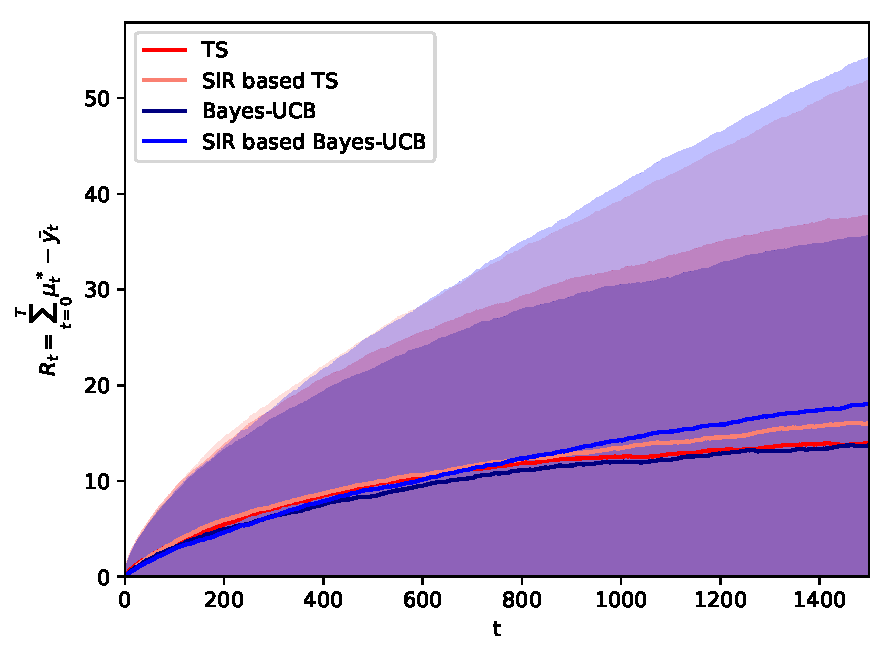
\includegraphics[width=\textwidth]{./figs/static/bernoulli/cumulative_regret}
		\caption{Bernoulli bandit, \\ $\theta_0=0.5,\theta_1=0.6$}
		\label{fig:static_bandits_bernoulli}
	\end{subfigure}
	\begin{subfigure}[b]{0.49\textwidth}
		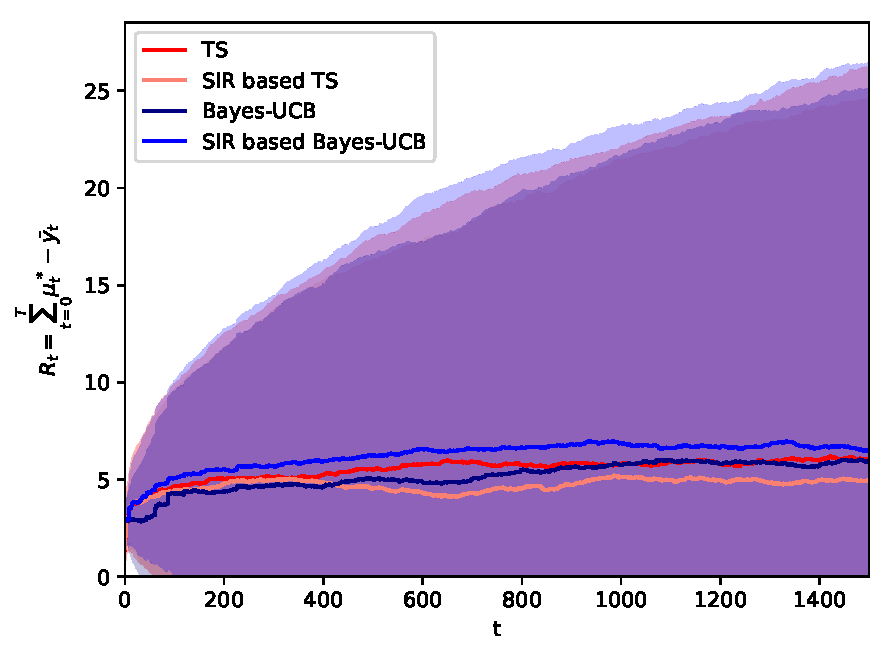
\includegraphics[width=\textwidth]{./figs/static/linearGaussian/cumulative_regret_known_sigma}
		\caption{Contextual linear-Gaussian bandit, \\ $\theta_0=(-1,-1),\theta_1=(1,1), \sigma^2=0.5$}
		\label{fig:static_bandits_linearGaussian}
	\end{subfigure}
	\caption{Mean regret (standard deviation shown as shaded region) in example static bandits.}
	\label{fig:static_bandits}
\end{figure}

\begin{figure}[!h]
	\begin{center}
		\centerline{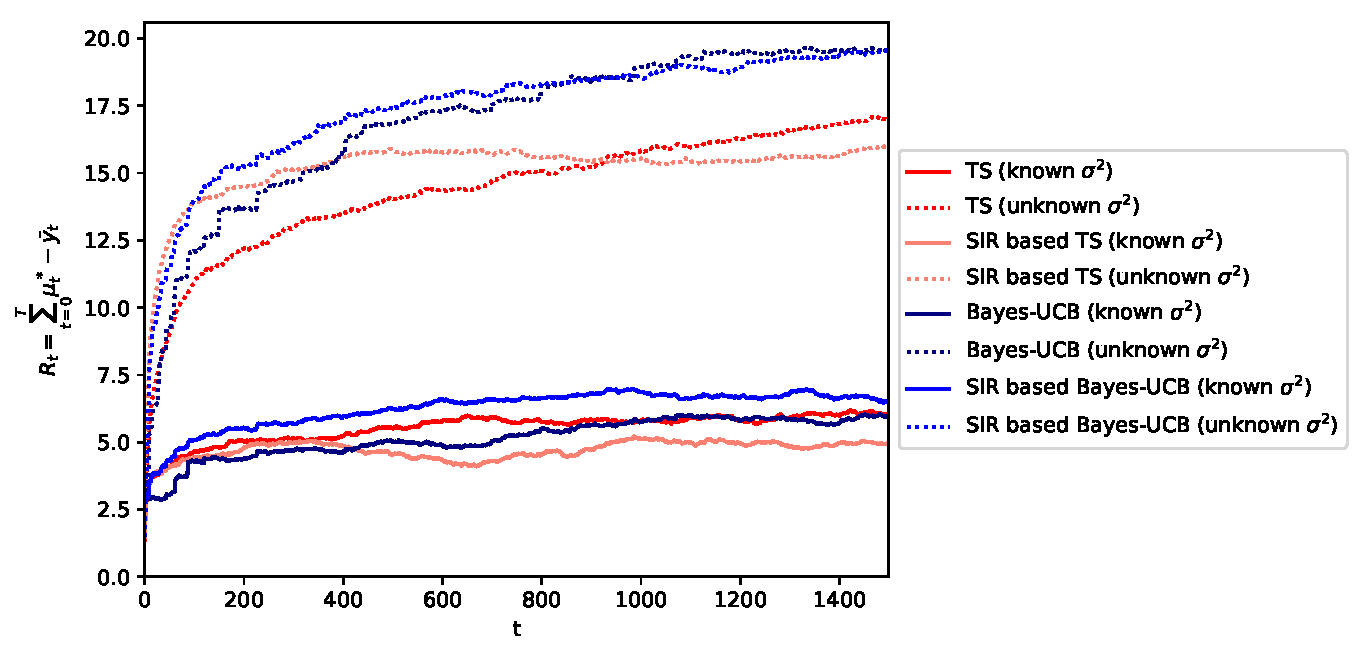
\includegraphics[width=\textwidth]{./figs/static/linearGaussian/cumulative_regret_all}}
		\caption{Mean regret for the contextual linear-Gaussian bandit $\theta_0=(-1,-1),\theta_1=(1,1)$ with unknown reward variance $\sigma^2=0.5$ and random contexts.}
		\label{fig:static_bandits_linearGaussian_all}
	\end{center}
\vspace*{-0.5cm}
\end{figure}

Note the increased uncertainty due to the MC approximation to the posterior, which finds its analytical justification in Eqn.~\eqref{eq:is_convergence}, and can be empirically reduced by increasing the number $M$ of IS samples used (see the impact of sample size $M$ in figures included in
\ifx\addappendix\undefined the supplementary material \else \autoref{asec:evaluation}\fi). $M=1000$ samples suffice in all our experiments for accurate estimation of parameter posteriors. Advanced and dynamic determination of SIR sample size is an active research area within the SMC community, but out of the scope of this paper.

We also evaluate a more realistic scenario for the contextual linear-Gaussian case with unknown reward variance $\sigma^2$ in Fig.~\ref{fig:static_bandits_linearGaussian_all}, where SIR-based approaches are shown to be competitive as well. We reiterate that results are satisfactory across a wide range of parameterizations and bandit sizes (results for extensive evaluations are provided in \ifx\addappendix\undefined the supplementary material \else \autoref{asec:evaluation} \fi), which validate the accuracy of the proposed SIR-based method.

Overall, the random measure approximation to the posteriors of the parameters of interest is accurate enough to allow for MAB policies to find the right exploration-exploitation tradeoff.

In several applications, binary rewards are well-modeled as depending on contextual factors \cite{ic-Chapelle2011,j-Scott2015}. The logistic reward function is suitable for these scenarios but, due to the unavailability of Bayesian closed-form posterior updates (see \ifx\addappendix\undefined the supplementary material \else \autoref{assec:logistic_rewards}\fi), one needs to resort to approximations, \eg the ad-hoc Laplace approximation proposed by \citet{ic-Chapelle2011}. 

Our proposed SIR-based framework is readily applicable, as one only needs to evaluate the logistic reward likelihood to compute the IS weights for the MAB policy of choice. Fig.~\ref{fig:static_bandits_logistic} shows how quickly SIR-based Thompson sampling and Bayes-UCB achieve the right exploration-exploitation tradeoff for different logistic parameterizations.

\begin{figure}[!ht]
	\centering
	\begin{subfigure}[b]{0.49\textwidth}
		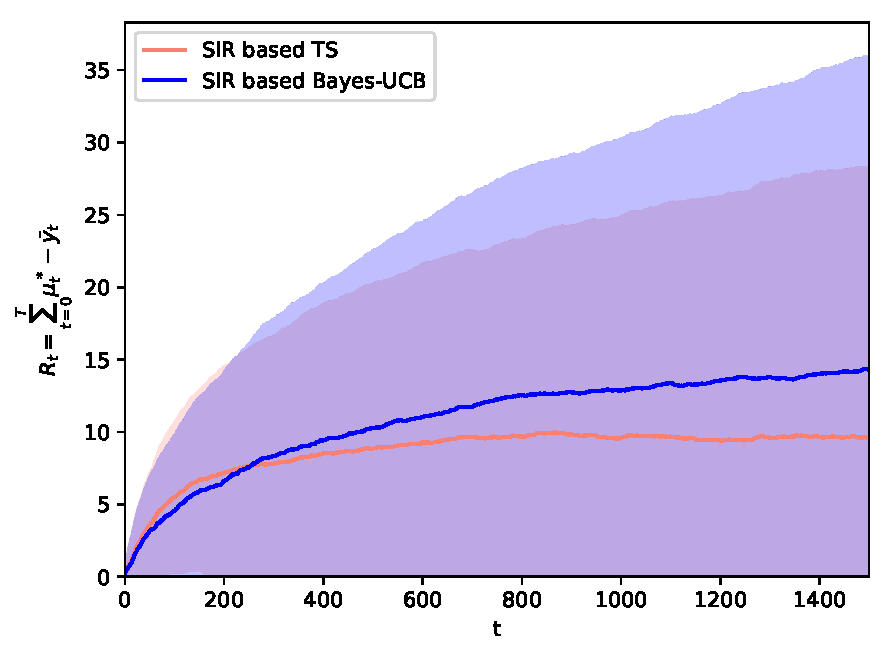
\includegraphics[width=\textwidth]{./figs/static/logistic/cumulative_regret_theta_05}
		\caption{Logistic bandit with $\theta_{0,i}=-0.5, \theta_{1,i}=0.5, \forall i$.}
		\label{fig:static_bandits_logistic_05}
	\end{subfigure}
	\begin{subfigure}[b]{0.49\textwidth}
		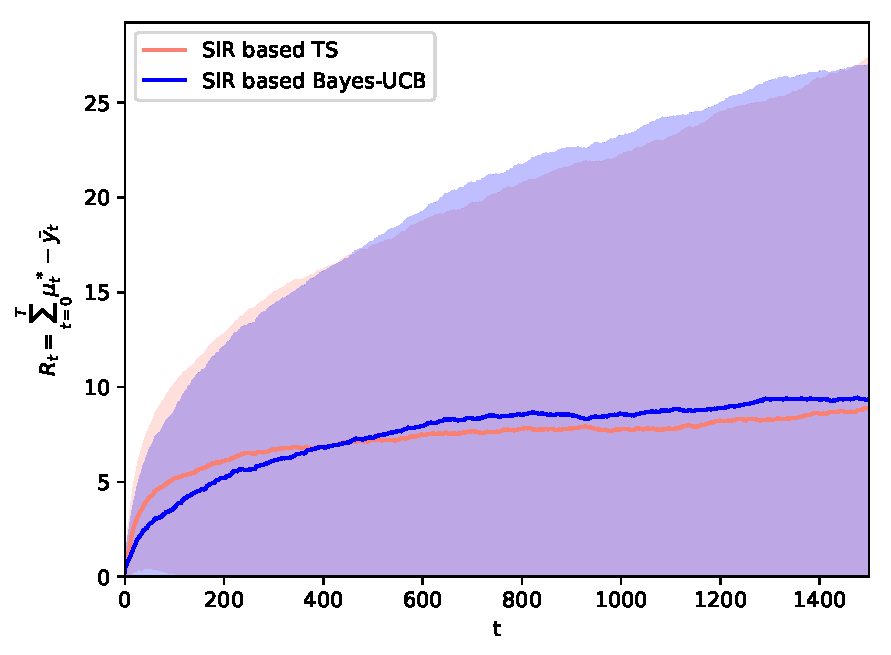
\includegraphics[width=\textwidth]{./figs/static/logistic/cumulative_regret_theta_1}
		\caption{Logistic bandit with $\theta_{0,i}=-1.0, \theta_{1,i}=1.0, \forall i$.}
		\label{fig:static_bandits_logistic_1}
	\end{subfigure}
	\caption{Mean regret (standard deviation shown as shaded region) in logistic bandits with random contexts.}
	\label{fig:static_bandits_logistic}
\end{figure}

These results indicate that the impact of only observing rewards of the played arms is minimal for the proposed SIR-based method. The parameter posterior uncertainty associated with the SIR-based estimation is automatically accounted for by both algorithms, as they explore rarely-played arms if the uncertainty is high. However, we do observe a slight performance deterioration of Bayes-UCB, which we argue is related to the quantile value used ($\alpha_t\propto1/t$). It was analytically justified by Kaufmann \cite{ip-Kaufmann2012} for Bernoulli rewards, but might not be optimal for other reward functions and, more importantly, for the SIR-based approximation to parameter posteriors.

On the contrary, Thompson sampling is more flexible, automatically adjusting to the uncertainty of the posterior approximation, and thus, attaining reduced regret.

\subsection{Dynamic bandits}
\label{ssec:dynamic_bandits}

Full potential of the proposed SIR-based algorithm is harnessed when facing the most interesting and challenging bandits: those with time-evolving parameters.

We consider the linear case (as formulated in Section~\ref{ssec:linear_mixing_dynamics}), because it allows us to (i) validate the SIR-based approximation to the optimal posterior (\ie the KF for the linear and Gaussian case); and (ii) show its flexibility and robustness to more realistic and challenging MAB models (with unknown parameters, nonlinear functions, and non-Gaussian distributions). 

We have evaluated different parameterizations of the model as in Eqn.~\eqref{eq:linear_mixing_dynamics} (all provided in
\ifx\addappendix\undefined the supplementary material \else \autoref{asec:evaluation}\fi),
but we here focus on a two-armed contextual dynamic bandit with parameters
\begin{equation}
\begin{split}
\begin{pmatrix}
\theta_{0,0,t}\\
\theta_{0,1,t}\\
\end{pmatrix} &= \begin{pmatrix}
0.9 & -0.1 \\
-0.1 & 0.9 \\
\end{pmatrix} \begin{pmatrix}
\theta_{0,0,t-1}\\
\theta_{0,1,t-1}\\
\end{pmatrix} + \epsilon_0 \; , \hspace*{1.47cm} \epsilon_0 \sim \N{\epsilon|0,0.1 \cdot\mathrm{I}} \;,\\
\begin{pmatrix}
\theta_{1,0,t}\\
\theta_{1,1,t}\\
\end{pmatrix} &= \begin{pmatrix}
0.9 & 0.1 \\
0.1 & 0.9 \\
\end{pmatrix} \begin{pmatrix}
\theta_{1,0,t-1}\\
\theta_{1,1,t-1}\\
\end{pmatrix} + \epsilon_1 \; , \hspace*{2.0cm} \epsilon_1 \sim \N{\epsilon|0,0.1 \cdot\mathrm{I}} \;.
\end{split}
\label{eq:dynamic_bandit_dynamics}
\end{equation}

\begin{figure}[!h]
	\begin{center}
		\centerline{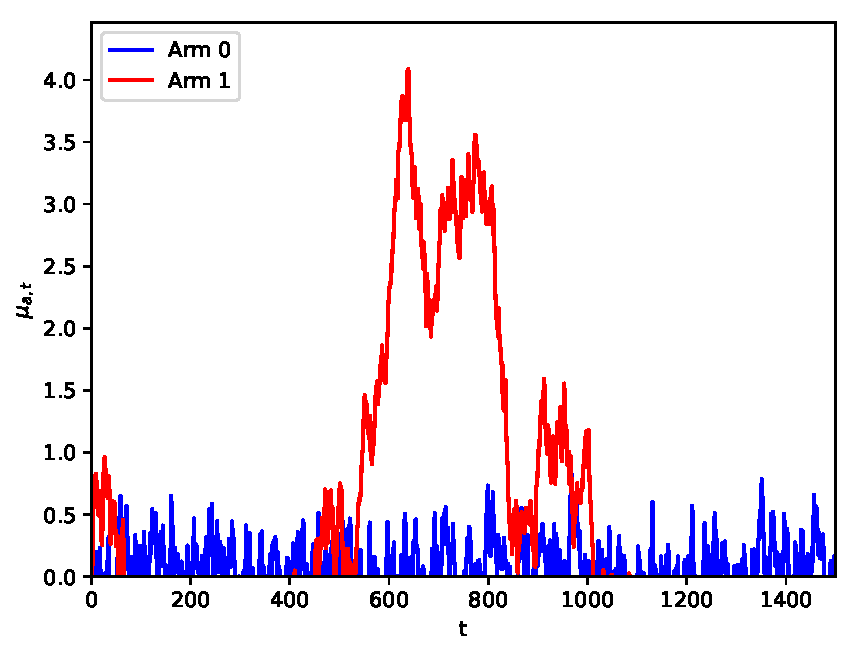
\includegraphics[width=0.6\columnwidth]{./figs/dynamic/dynamics}}
		\caption{Expected per-arm rewards over time for a contextual linear dynamic bandit. Note how the optimal arm switches around $t=\{50, 500, 1000\}$.}
		\label{fig:dynamic_bandits_dynamics}
	\end{center}
\vspace*{-0.5cm}
\end{figure}

Fig.~\ref{fig:dynamic_bandits_dynamics} illustrates the time-evolution of the expected rewards for a realization of Eqn.~\eqref{eq:dynamic_bandit_dynamics}. We consider this setting of special interest because the induced expected rewards change over time and so, the decision on the optimal arm swaps accordingly. We evaluate the proposed SIR-based methods for bandits with dynamics as in Eqn.~\eqref{eq:dynamic_bandit_dynamics}, and both contextual linear-Gaussian and logistic rewards. 

We show in Fig.~\ref{fig:dynamic_bandits_linearGaussian_dknown} that the regret of SIR-based methods, for the contextual linear-Gaussian case with known parameters, is equivalent to the optimal case (\ie the KF). Furthermore, even for the scenarios where the reward variance $\sigma^2$ is unknown, and thus the Gaussianity assumption needs to be dropped (instead modeling bandit rewards via Student-t distributions), SIR-based methods perform comparably well.

\begin{figure}[!h]
	\centering
	\begin{subfigure}[b]{0.49\textwidth}
		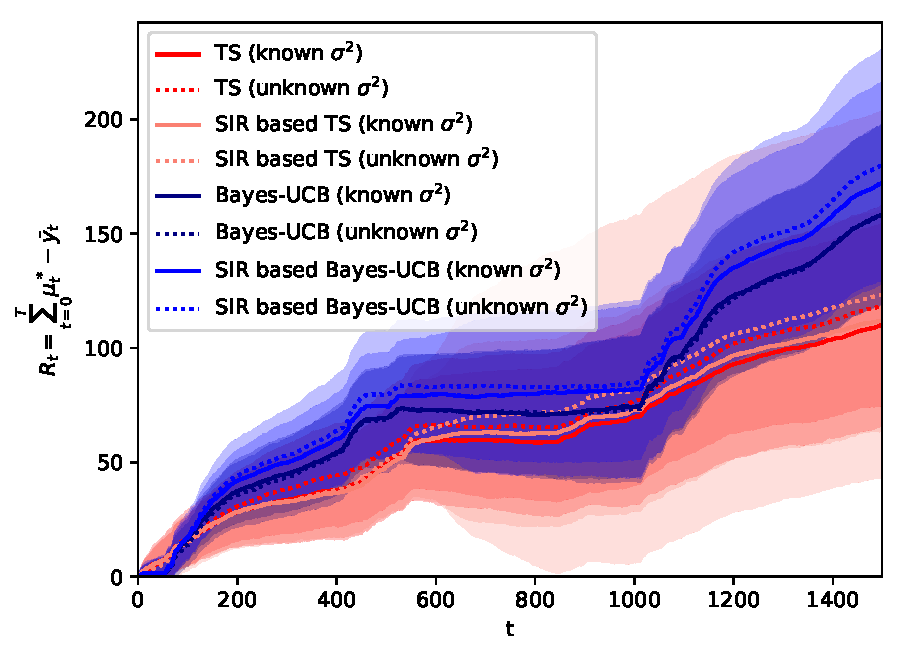
\includegraphics[width=\textwidth]{./figs/dynamic/linearGaussian/cumulative_regret_all_dknown_cstatic}
		\caption{Static context.}
		\label{fig:dynamic_bandits_linearGaussian_cstatic_dknown}
	\end{subfigure}
	\begin{subfigure}[b]{0.49\textwidth}
		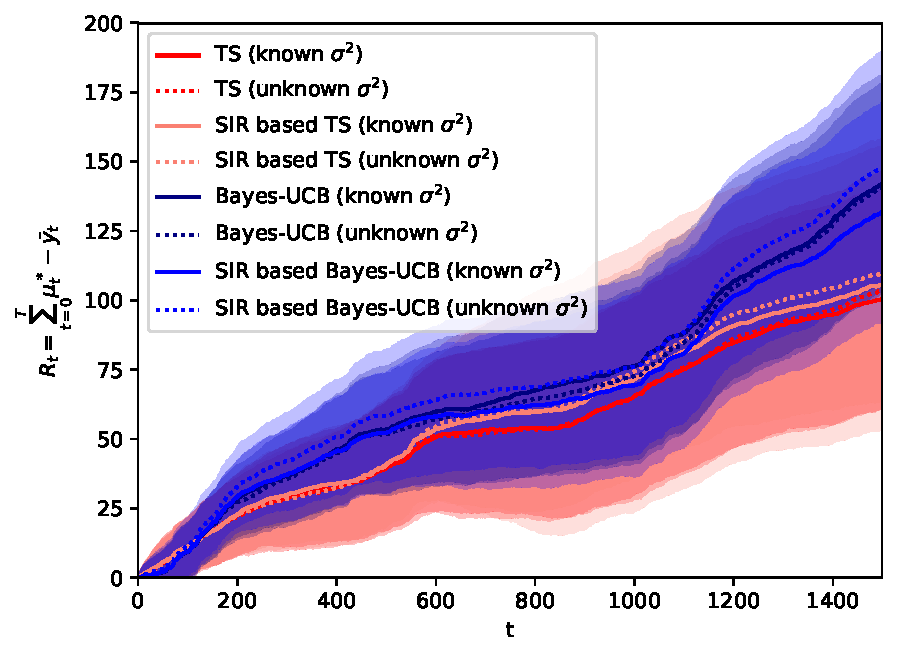
\includegraphics[width=\textwidth]{./figs/dynamic/linearGaussian/cumulative_regret_all_dknown_crand}
		\caption{Uniformly random context.}
		\label{fig:dynamic_bandits_linearGaussian_crand_dknown}
	\end{subfigure}
	\caption{Mean regret (standard deviation shown as shaded region) in contextual linear-Gaussian bandits with known dynamics. Notice the regret bumps when optimal arms swap at $t=\{500, 1000\}$, and how our proposed SIR-based methods adjust.}
	\label{fig:dynamic_bandits_linearGaussian_dknown}
\end{figure}

Finally, we evaluate in Fig.~\ref{fig:dynamic_bandits_linearGaussian_dunknown} the most challenging contextual linear-Gaussian bandit case, where none of the parameters of the model ($A,C,\sigma^2$) are known; \ie one must sequentially learn the underlying dynamics, in order to make informed online decisions. Due to the flexibility of SIS in approximating the key parameter posteriors, SIR-based Thompson sampling and Bayes-UCB are both able to accurately learn their evolution and thus, reach the exploitation-exploration balance.

\begin{figure}[!h]
	\begin{subfigure}[b]{0.49\textwidth}
		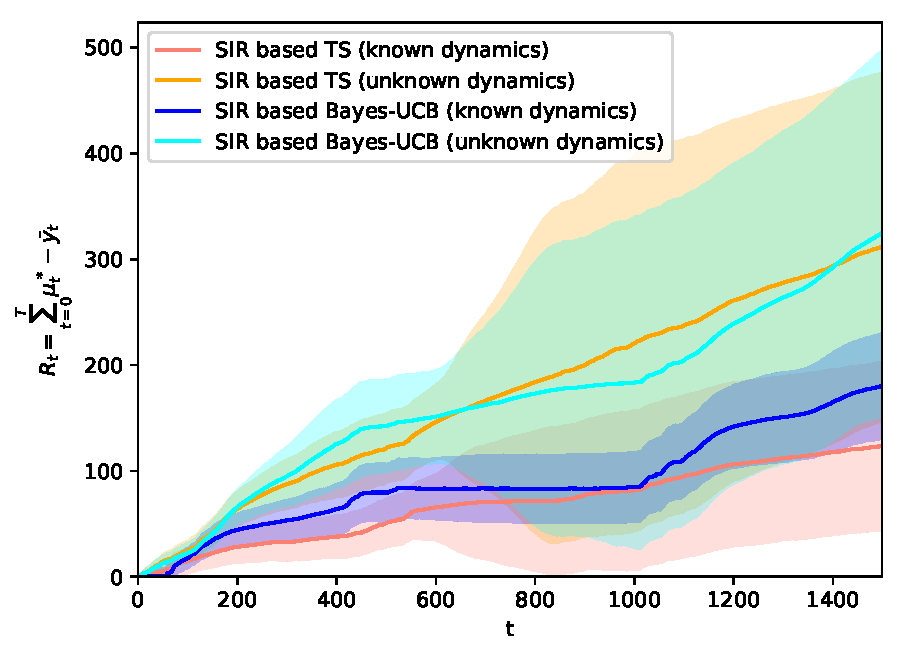
\includegraphics[width=\textwidth]{./figs/dynamic/linearGaussian/cumulative_regret_all_dunknown_cstatic}
		\caption{Static context.}
		\label{fig:dynamic_bandits_linearGaussian_cstatic_dunknown}
	\end{subfigure}
	\begin{subfigure}[b]{0.49\textwidth}
		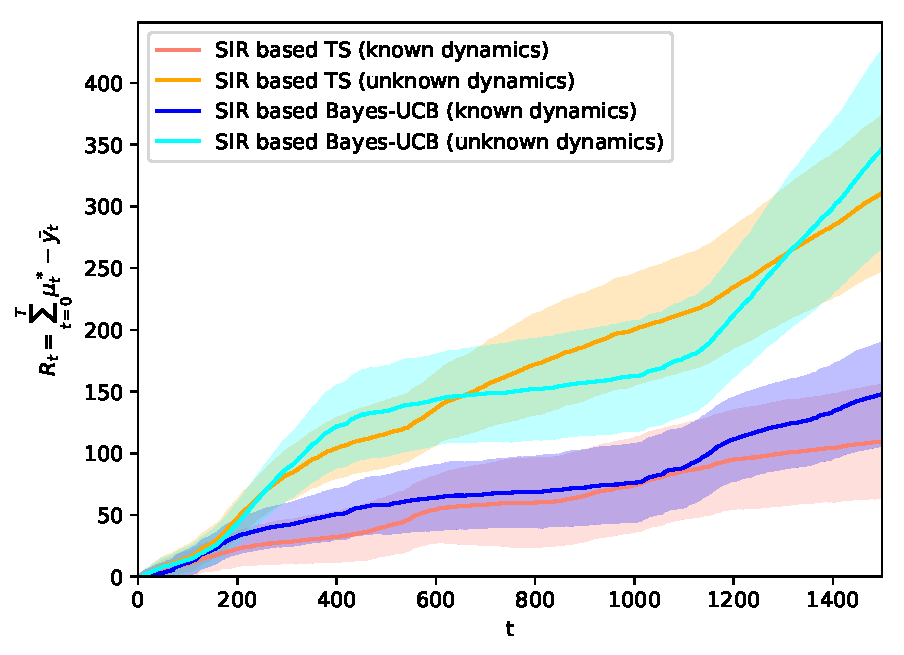
\includegraphics[width=\textwidth]{./figs/dynamic/linearGaussian/cumulative_regret_all_dunknown_crand}
		\caption{Uniformly random context.}
		\label{fig:dynamic_bandits_linearGaussian_crand_dunknown}
	\end{subfigure}
	\caption{Mean regret (standard deviation shown as shaded region) in contextual linear-Gaussian bandits with unknown dynamics. Notice the regret bumps when optimal arms swap at $t=\{500, 1000\}$, and how our proposed SIR-based methods adjust.}
	\label{fig:dynamic_bandits_linearGaussian_dunknown}
\end{figure}

We observe noticeable increases in regret when the dynamics of the parameters (as in Fig.~\ref{fig:dynamic_bandits_dynamics}) swap the optimal arm. Note that these changes in parameter dynamics impact Bayes-UCB more profoundly as time evolves. This effect is also observed for linearly dynamic bandits with logistic reward functions (see Fig.~\ref{fig:dynamic_bandits_logistic} for logistic rewards with both static and random contexts).

\begin{figure}[!h]
	\begin{subfigure}[b]{0.49\textwidth}
		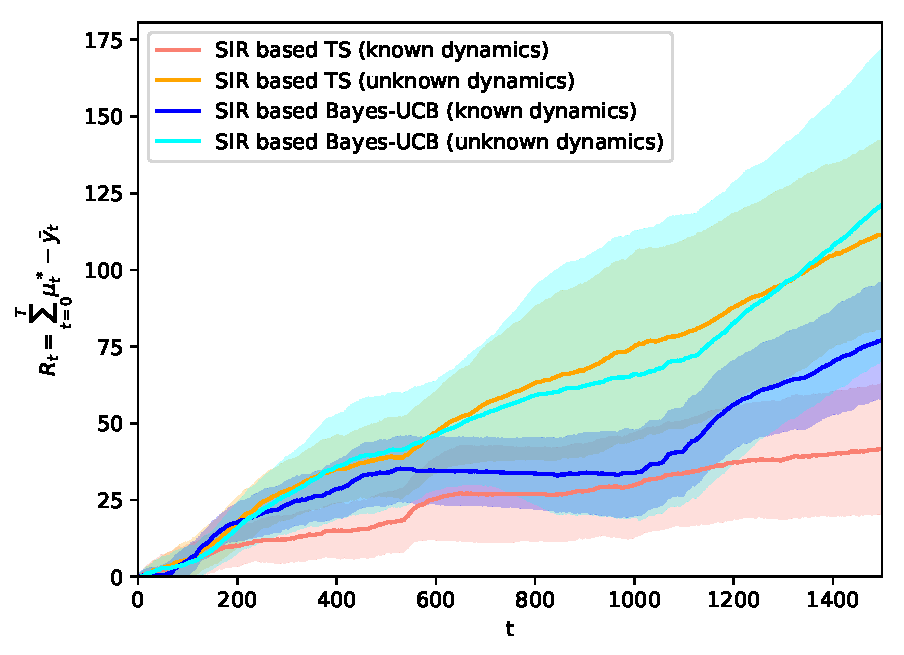
\includegraphics[width=\textwidth]{./figs/dynamic/logistic/cumulative_regret_all_cstatic}
		\caption{Static context.}
		\label{fig:dynamic_bandits_logistic_cstatic}
	\end{subfigure}
	\begin{subfigure}[b]{0.49\textwidth}
		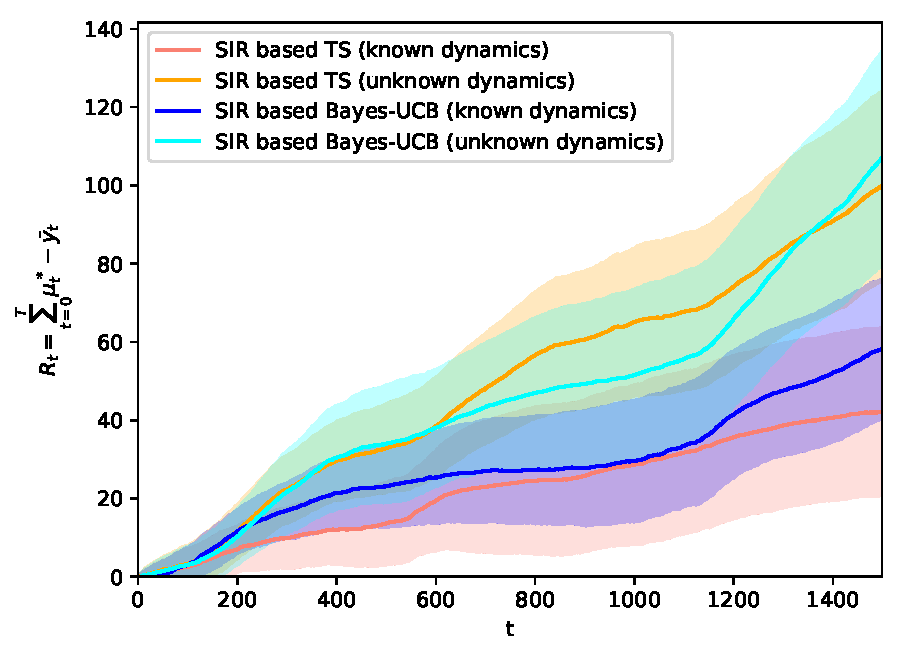
\includegraphics[width=\textwidth]{./figs/dynamic/logistic/cumulative_regret_all_crand}
		\caption{Uniformly random context.}
		\label{fig:dynamic_bandits_logistic_crand}
	\end{subfigure}
	\caption{Mean regret (standard deviation shown as shaded region) in contextual linear logistic dynamic bandits. Notice the regret bumps when optimal arms swap at $t=\{500, 1000\}$, and how our proposed SIR-based methods adjust.}
	\label{fig:dynamic_bandits_logistic}
\end{figure}

We argue that the shrinking quantile value $\alpha_t\propto1/t$ explains this behavior. It was originally proposed in \cite{ip-Kaufmann2012} based on confidence bounds of static reward models, which tend to shrink with more observations of the bandit. However, the uncertainty of the evolving parameter posteriors (due to the dynamics of unobserved arms) might result in broader distributions and thus, the inadequacy of the shrinking $\alpha_t$. More generally, the need to determine appropriate quantile values $\alpha_t$ for each model is a drawback for Bayes-UCB type algorithms.

On the contrary, Thompson sampling does not require any parameter tweaking. It relies on samples from the posterior, which SIR is able to approximate accurately enough for it to operate successfully, even in the most challenging MAB scenarios as in Figs.~\ref{fig:dynamic_bandits_linearGaussian_dunknown} and \ref{fig:dynamic_bandits_logistic}.

Due to the Bayesian approach to MAB, our proposed SIR-based Thompson sampling not only estimates the evolving parameters $\theta_t$, but also their corresponding uncertainty. As such, both when a given arm's dynamics are unclear, or when an arm is not sampled for a while, the uncertainty of its estimated posterior grows. As a result, Thompson sampling is more likely to explore that arm again, in order to achieve the right exploration-exploitation balance, as shown in our results.

\subsection{Bandits for personalized news article recommendation}
\label{ssec:logged_data_bandits}

Finally, we consider the application of the proposed SIR-based methods for recommendation of personalized news articles, in a similar fashion as done by \citet{ic-Chapelle2011}. Online content recommendation represents an important example of reinforcement learning, as it requires efficient balancing of the exploration and exploitation tradeoff.

We use a dataset\footnote{Available at \href{https://webscope.sandbox.yahoo.com/catalog.php?datatype=r\&did=49}{R6A - Yahoo! Front Page Today Module User Click Log Dataset.}} that contains a fraction of user click logs for news articles displayed in the Featured Tab of the Today Module on Yahoo! Front Page during the first ten days in May 2009. The articles to be displayed were originally chosen uniformly at random from a hand-picked pool of high-quality articles. As such, the candidate pool was originally dynamic. However, we picked a subset of 20 articles shown in May 08th and collected all logged user interactions, for a total of 500354.

The goal is to choose the most interesting article to users, or in bandit terms, to maximize the total number of clicks on the recommended articles, \ie the average click-through rate (CTR). In the dataset, each user is associated with six features: a bias term and 5 features that correspond to the membership features constructed via the conjoint analysis with a bilinear model described in \cite{ip-Chu2009}.

We treat each article as an arm ($A=20$), and the logged reward is whether the article is clicked or not by the user ($y_t=\{1,0\}$). We pose the problem as a MAB with logistic rewards, so that we can account for the user features ($x_t\in \Real^6$).

One may further hypothesize that the news recommendation system should evolve over time, as the relevance of news might change during the course of the day. As a matter of fact, our proposed framework readily accommodates these assumptions.

We consider both static and dynamic bandits with logistic rewards, and implement the proposed SIR-based Thompson sampling, due to its flexibility and the lack of parameter tuning required. Summary CTR results are provided in Table \ref{tab:yahoo_logistic_crt}. Observe the flexibility of the dynamic bandit, which is able to pick up the dynamic popularity of certain articles over time (see Fig. \ref{fig:yahoo_logistic_dynamic}).


\begin{figure}[!hb]
	\centering
	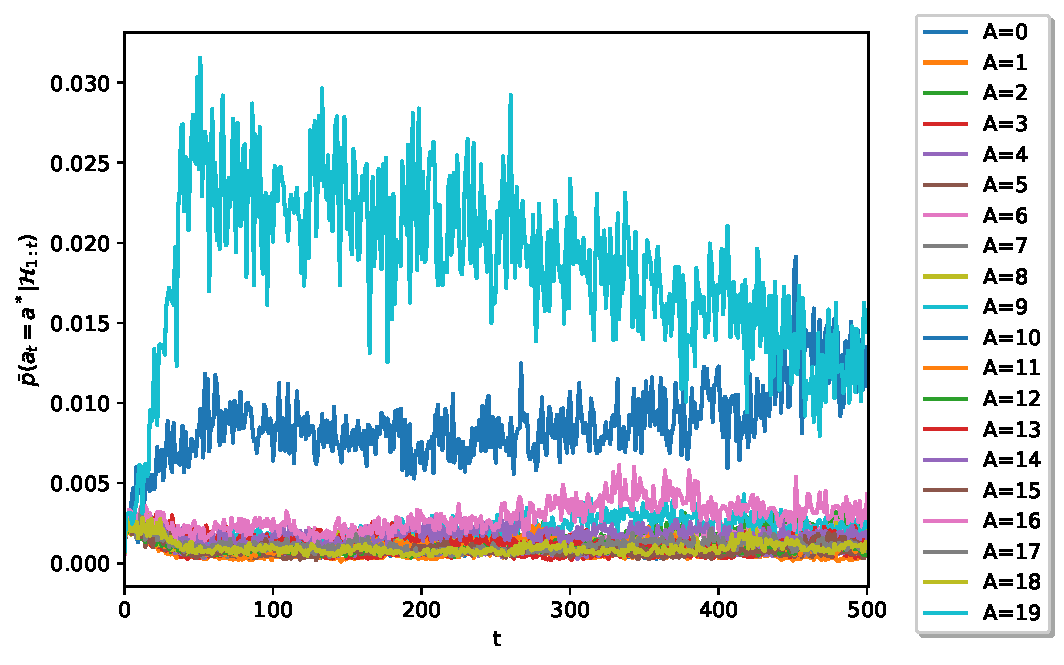
\includegraphics[width=0.95\textwidth]{./figs/yahoo/yahoo_logistic_dynamic}
	\caption{Empirical probability of SIR-based contextual dynamic logistic Thompson sampling policy picking each arm over time. Notice how the algorithm captures the changing popularity of articles over time.}
	\label{fig:yahoo_logistic_dynamic}
\end{figure}

%%%%%%%%%%%%%%%%%%%%%%%%
%% Table for yahoo data with logistic bandits
%%%%%%%%%%%%%%%%%%%%%%%%
\begin{table}[!h]
	\begin{center}
			\begin{tabular}{*{4}{|c}|}
				\hline
				% Header
				\multicolumn{2}{|c|}{\multirow{2}{*}{}} & CTR\cellcolor[gray]{0.6} & Normalized CTR\cellcolor[gray]{0.6} \\ \hline
				% table starts
				\cellcolor[gray]{0.6} & \cellcolor[gray]{0.8} Logistic rewards, static arms & 0.0670 +/- 0.0088 & 1.6149 +/- 0.2313  \\ \cline{1-4}
				\cellcolor[gray]{0.6} & \cellcolor[gray]{0.8} Logistic rewards, time-evolving arms & 0.0655 +/- 0.0082 & 1.5765 +/- 0.2042 \\ \cline{1-4}
				\multicolumn{1}{c}{\multirow{-4}{*}{Model}} & \multicolumn{3}{c}{}
			\end{tabular}
		\caption{CTR results for SIR-based bandits on the news article recommendation data. The normalized CTR is with respect to a random baseline.}
		\vspace*{-1cm}
		\label{tab:yahoo_logistic_crt}
	\end{center}
\end{table}

\section{Conclusion}
\label{sec:conclusion}

We have presented a (sequential) importance sampling-based framework for the MAB problem, where we combine sequential Monte Carlo inference with state-of-the-art Bayesian MAB policies. The proposed algorithmic setting allows for interpretable modeling of complex reward functions and time-evolving bandits. The methods sequentially learn the dynamics of the bandit from online data, and are able to find the exploration-exploitation balance.

In summary, we extend the applicability of Bayesian MAB policies (Thompson sampling and Bayes-UCB in particular) by accommodating complex models of the world with SIR-based inference of the unknowns. Empirical results show good cumulative regret performance of the proposed framework in simulated challenging models (\eg contextual logistic dynamic bandits), and practical scenarios (personalized news article recommendation) where complex models of data are required.

\subsection{Software and Data}
The implementation of the proposed method is available in \href{https://github.com/iurteaga/bandits}{this public repository}. It contains all the software required for replication of the findings of this study.

\subsubsection*{Acknowledgments}
This research was supported in part by NSF grant SCH-1344668.
We thank Luke Bornn for bringing \cite{j-Cherkassky2013}  to our attention.

% Generate bibliography from the specified bibliography file
\bibliography{../literature}
% Select a .bst file for the style
\bibliographystyle{abbrvnat}

%%%%%%%%%%%%%%%%%%%%%%%%%%%%%%%%%%%%%%%%%%%%%%%%%%%%%%%%%%%%%%%%%%%%%%%%%%%%%%%
%%%%%%%%%%%%%%%%%%%%%%%%%%%%%%%%%%%%%%%%%%%%%%%%%%%%%%%%%%%%%%%%%%%%%%%%%%%%%%%
% Whether to add appendix or not
\ifx\addappendix\undefined \end{document} \else \iftrue \fi

\clearpage
\appendix
\section{MAB models}
\label{asec:bandit_models}

We now describe the key distributions for some MAB models of interest.

\subsection{Bernoulli rewards}
\label{assec:bernoulli_rewards}

The Bernoulli distribution is well suited for applications with binary returns (\ie success or failure of an action) that don't depend on a context. The rewards $y\in\{0,1\}$ of each arm are modeled as independent draws from a Bernoulli distribution with success probabilities $\theta_a$, \ie
\begin{equation}
p_a(y|\theta)=\Ber{y|\theta_a}=\theta_a^{y}(1-\theta_a)^{(1-y)} \;.
\end{equation}

For this reward distribution, the parameter conjugate prior distribution is the Beta distribution
\begin{equation}
\begin{split}
p(\theta_a|\alpha_{a,0}, \beta_{a,0})&=\Beta{\theta_a|\alpha_{a,0}, \beta_{a,0}} =\frac{\Gamma\left(\alpha_0+\beta_0\right)}{\Gamma\left(\alpha_0\right)\Gamma\left(\beta_0\right)} \theta_a^{\alpha_0-1}(1-\theta_0)^{\beta_0-1} \; .
\end{split}
\end{equation} 

After observing actions $a_{1:t}$ and rewards $y_{1:t}$, the parameter posterior follows an updated Beta distribution
\begin{equation}
\begin{split}
p(\theta_a|a_{1:t}, y_{1:t}, \alpha_{a,0}, \beta_{a,0}) &= p(\theta_a|\alpha_{a,t}, \beta_{a,t}) =\Beta{\theta_a|\alpha_{a,t}, \beta_{a,t}}\; ,
\end{split}
\end{equation}
with sequential updates
\begin{equation}
\begin{cases}
\alpha_{a,t}=\alpha_{a,t-1} + y_{t} \cdot \mathds{1}[a_t=a] \; ,\\
\beta_{a,t}=\beta_{a,t-1} + (1 - y_{t}) \cdot \mathds{1}[a_t=a] \; ,
\end{cases} 
\end{equation}
or, alternatively, batch updates
\begin{equation}
\begin{cases}
\alpha_{a,t}=\alpha_{a,0} + \sum_{t|a_t=a} y_{t} \; ,\\
\beta_{a,t}=\beta_{a,0} + \sum_{t|a_t=a} (1-y_{t}) \; .
\end{cases}
\end{equation}

The expected reward for each arm follows
\begin{equation}
p(\mu_{a}|\theta_a)=p(\theta_{a}|a_{1:t},y_{1:t})=\Beta{\theta_a|\alpha_{a,t}, \beta_{a,t}} \; ,
\end{equation}
and the quantile function is based on the Beta distribution
\begin{equation}
q_{a,t+1}(\alpha_{t+1})=Q\left(1-\alpha_{t+1}, \Beta{\theta_a|\alpha_{a,t}, \beta_{a,t}}\right) \;.
\end{equation}

\subsection{Contextual linear-Gaussian rewards}
\label{assec:linear_gaussian_rewards}

For bandits with continuous rewards, the Gaussian distribution is often applicable, where contextual dependencies can also be included. The contextual linear-Gaussian reward model is suited for these scenarios, where the expected reward of each arm is modeled as a linear combination of a $d$-dimensional context vector $x\in\Real^{d}$ and the idiosyncratic parameters of the arm $w_a\in\Real^{d}$, \ie
\begin{equation}
\begin{split}
p_a(y|x,\theta)&=\N{y|x^\top w_a, \sigma_a^2} =\frac{e^{-\frac{(y-x^\top w_a)^2}{2\sigma_a^2}}}{\sqrt{2\pi\sigma_a^2}} \; .
\end{split}
\end{equation}
We denote as $\theta\equiv\{w, \sigma\}$ the set of all the parameters.

For this reward distribution, the parameter conjugate prior distribution is the Normal Inverse Gamma distribution
\begin{equation}
\begin{split}
p(w_a, \sigma_a^2|u_{a,0}, V_{a,0}, \alpha_{a,0}, \beta_{a,0}) &= \NIG{w_a, \sigma_a^2|u_{a,0}, V_{a,0},\alpha_{a,0}, \beta_{a,0}} \\
& = \N{w_a|u_{a,0}, \sigma_a^2 V_{a,0}} \cdot \Gamma^{-1}{\sigma_a^2|\alpha_{a,0}, \beta_{a,0}} \\
& = \frac{e^{-\frac{1}{2}(w_a-u_{a,0})^\top(\sigma_a^2 V_{a,0})^{-1}(w_a-u_{a,0})}}{(2\pi)^{1/2}\sigma_a \mydet{V_{a,0}}^{-1/2}} \cdot \frac{\beta_0^{\alpha_0}}{\Gamma\left(\alpha_0\right)} (\sigma_a^2)^{-\alpha_0-1}e^{-\frac{\beta_0}{(\sigma_a^2)}} \; .
\end{split}
\end{equation}

After observing actions $a_{1:t}$ and rewards $y_{1:t}$, the parameter posterior follows an updated NIG distribution
\begin{equation}
\begin{split}
p(w_a, \sigma_a^2|a_{1:t},y_{1:t},u_{a,0}, V_{a,0},\alpha_{a,0}, \beta_{a,0}) &= p\left(w_a, \sigma_a^2|u_{a,t}, V_{a,t},\alpha_{a,t}, \beta_{a,t}\right) \\
&=\NIG{w_a, \sigma_a^2|u_{a,t}, V_{a,t},\alpha_{a,t}, \beta_{a,t}} \; ,
\end{split}
\end{equation}
with sequential updates
\begin{equation}
\begin{cases}
V_{a,t}^{-1} = V_{a,t-1}^{-1} + x_t x_t^\top \cdot \mathds{1}[a_t=a] \; ,\\
u_{a,t}= V_{a,t} \left( V_{a,t-1}^{-1} u_{a,t-1} + x_t y_{t}\cdot \mathds{1}[a_t=a]\right) \; ,\\
\alpha_{a,t}=\alpha_{a,t-1} + \frac{\mathds{1}[a_t=a]}{2} \; ,\\
\beta_{a,t}=\beta_{a,t-1} + \frac{\mathds{1}[a_t=a](y_{t_a}-x_t^\top u_{a,t-1})^2}{2\left(1+x_t^\top V_{a,t-1} x_t\right)} \; ,
\end{cases}
\end{equation}
or, alternatively, batch updates
\begin{equation}
\begin{cases}
V_{a,t}^{-1}= V_{a,0}^{-1}+x_{{1:t}|t_a} x_{{1:t}|t_a}^\top \; ,\\
u_{a,t}=V_{a,t}\left(V_{a,0}^{-1}u_{a,0}+x_{{1:t}|t_a} y_{{1:t}|t_a}\right) \; ,\\
\alpha_{a,t}=\alpha_{a,0} + \frac{|t_a|}{2} \; ,\\
\beta_{a,t}=\beta_{a,0} + \frac{\left(y_{{1:t}|t_a}^\top y_{{1:t}|t_a} + u_{a,0}^\top V_{a,0}^{-1}u_{a,0} - u_{a,t}^\top V_{a,t}^{-1}u_{a,t} \right)}{2} \; ,
\end{cases}
\end{equation}
where $t_a=\{t|a_t=a\}$ indicates the set of time instances when arm $a$ is played.

The expected reward for each arm follows
\begin{equation}
p(\mu_{a}|x, \sigma_a^2, u_{a,t}, V_{a,t}) = \N{\mu_{a}|x^\top u_{a,t}, \; \sigma_a^2 \cdot x^\top V_{a,t} x}.
\end{equation}
and the quantile function is based on this Gaussian distribution
\begin{equation}
\resizebox{0.48\textwidth}{!}{$
	q_{a,t+1}(\alpha_{t+1})=Q\left(1-\alpha_{t+1}, \N{\mu_{a}|x^\top u_{a,t}, \; \sigma_a^2 \cdot x^\top V_{a,t} x}\right) \;.
	$}
\end{equation}

For the more realistic scenario where the reward variance $\sigma^2_a$ is unknown, we can marginalize it and obtain
\begin{equation}
\begin{split}
p(\mu_{a}|x, u_{a,t}, \sigma_a^2, V_{a,t}) & = \T{\mu_{a}|2\alpha_{a,t}, x^\top u_{a,t}, \; \frac{\beta_{a,t}}{\alpha_{a,t}} \cdot x^\top V_{a,t} x} \\
& = \frac{\Gamma\left(\frac{2\alpha_{a,t}+1}{2}\right)}{\Gamma\left(\frac{2\alpha_{a,t}}{2}\right)\sqrt{\pi 2\alpha_{a,t} \frac{\beta_{a,t}}{\alpha_{a,t}} x^\top V_{a,t} x}} \cdot \left(1+\frac{1}{(2\alpha_{a,t})}\left(\frac{(\mu_a-x^\top u_{a,t})^2}{\frac{\beta_{a,t}}{\alpha_{a,t}} \cdot x^\top V_{a,t} x}\right)\right)^{-\frac{2\alpha_{a,t}+1}{2}} \; .
\end{split}
\end{equation}
The quantile function for this case is based on the Student's-t distribution
\begin{equation}
\resizebox{0.48\textwidth}{!}{$
	q_{a,t+1}(\alpha_{t+1})=Q\left(1-\alpha_{t+1}, \T{\mu_{a}| 2\alpha_{a,t}, x^\top u_{a,t}, \; \frac{\beta_{a,t}}{\alpha_{a,t}} \cdot x^\top V_{a,t} x}\right) \;.
	$}
\end{equation}

Note that one can use the above results for bandits with no context, by replacing $x=I$ and obtaining $\mu_{a}=u_{a,t}$.

\subsection{Contextual linear logistic rewards}
\label{assec:logistic_rewards}

The logistic function is applicable for problems where returns are binary (\ie success or failure of an action), but depend on a $d$-dimensional context vector $x\in\Real^{d}$ and idiosyncratic parameters of each arm $\theta_a$. The contextual linear logistic reward model follows
\begin{equation}
p_a(y|x,\theta)=\frac{e^{y\cdot(x^\top\theta_a) }}{1+e^{(x^\top\theta_a)}} \; .
\end{equation}

For this reward distribution, the posterior of the parameters can not be computed in closed form and, neither, the quantile function of the expected rewards $\mu_a=y\cdot(x^\top\theta_a)$.

\subsection{Linearly dynamic bandits}
\label{assec:linear_mixing_dynamics}

Let us consider a general linear model for the dynamics of the parameters of each arm $\theta_{a} \in \Real^{d}$:
\begin{equation}
\theta_{a,t}=L_a \theta_{a,t-1}+\epsilon_a \;, \qquad \epsilon_a\sim\N{\epsilon_a|0, C_a} \; ,
\end{equation}
where $L_a \in \Real^{d \times d}$ and $C_a \in \Real^{d \times d}$. One can immediately determine that, for linearly dynamic bandits with known parameters, the parameters follow
\begin{equation}
\theta_{a,t}\sim \N{\theta_{a,t}|L_a \theta_{a,t-1}, C_a} \; .
\end{equation}

However, it is unrealistic to assume that the parameters are known in practice. We thus marginalize them out by means of the following conjugate priors for the matrix $A$ and covariance matrix $C$ (we drop the per arm subscript $a$ for clarity)
\begin{equation}
\begin{split}
p(A,C|L_0, B_0, \nu_0, V_0) &= \NIW{A,C|L_0, B_0, \nu_0, V_0} = p(A|L_0, B_0, C) p(C|\nu_0, V_0) \\
& =\MN{A|L_0, C, B_0} \IW{C|\nu_0, V_0} \; ,
\end{split}
\end{equation}
where the matrix variate Gaussian distribution follows
\begin{equation}
\MN{A|L_0, C, B_0}= \frac{e^{-\frac{1}{2} \tr{B_0^{-1} \left(A-L_0\right)^\top C^{-1}\left(A-L_0\right)}}}{(2\pi)^{(d\cdot d)/2}\mydet{B_0}^{d/2}\mydet{C}^{d/2}} \; ,
\end{equation}
and the Inverse Wishart
\begin{equation}
\IW{C|\nu_0,V_0}=\frac{\mydet{C}^{-\frac{\nu_0+d+1}{2}} e^{-\frac{1}{2} \tr{C^{-1} V_0}}}{2^{\frac{\nu_0\cdot d}{2}}\mydet{V_0}^{-\frac{\nu_0}{2}}\Gamma\left(\frac{\nu_0}{2}\right)} \; .
\end{equation}

We integrate out the unknown parameters $A$ and $C$ to derive the predictive density, \ie the distribution of $\theta_{t}$, given all the past data $\theta_{1:t}$. One can show that the resulting distribution is a multivariate t-distribution
\begin{equation}
\begin{split}
f(\theta_{t}|\theta_{1:t-1}) &= \T{\theta_{t}|\nu_{t}, m_{t}, R_{t}} \propto \mydet{1+\frac{1}{\nu_{t}}\left(\theta_{t}-m_{t}\right)R_{t}^{-1}\left(\theta_{t}-m_{t}\right)^\top}^{-\frac{\nu_{t}+d}{2}} \; ,
\end{split}
\end{equation}
where $\nu_{t}$ denotes degrees of freedom, $m_{t} \in \Real^{d}$ is the location parameter, and $R_{t}\in \Real^{d\times d}$ represents the scale matrix \cite{b-Bernardo2009}. These follow
\begin{equation}
\begin{cases}
\nu_{t}=\nu_{0}+t-d \; ,\\
m_{t}=L_{t-1} \theta_{t-1} \; , \\
R_{t} = \frac{V_{t-1}}{\nu_{t}\left(1-\theta_{t-1}^\top(U U^\top)^{-1}\theta_{t-1}\right)} \; ,\\
\end{cases}
\end{equation}
where the sufficient statistics of the parameters are
\begin{equation}
\begin{cases}
B_{t-1} = \left(\Theta_{0:t-2}\Theta_{0:t-2}^\top + B_0^{-1} \right)^{-1} \; ,\\
L_{t-1} = \left(\Theta_{1:t-1}\Theta_{0:t-2}^\top+A_0B_0^{-1}\right) B_{t-1} \; ,\\
V_{t-1}= \left(\Theta_{1:t-1}-L_{t-1} \Theta_{0:t-2}\right)\left(\Theta_{1:t-1}-L_{t-1} \Theta_{0:t-2}\right)^\top \\
\qquad \qquad + \left(L_{t-1}-L_0\right) B_0^{-1} \left(L_{t-1}-L_0\right)^\top + V_0 \; ,\\
U U^\top = \left(\theta_{t-1}\theta_{t-1}^\top+B_{t-1}^{-1}\right) \; ,\\
\end{cases}
\end{equation}
and we have defined the stacked parameter matrix
\begin{equation}
\Theta_{t_0:t_1}=[\theta_{t_0} \theta_{t_0+1} \cdots \theta_{t_1-1} \theta_{a,t_1}] \in \Real^{d\times (t_1-t_0)} \; .
\end{equation}

All in all, for linear dynamic bandits with unknown parameters, the per-arm parameters follow
\begin{equation}
\theta_{a,t} \sim \T{\theta_{a,t}|\nu_{a,t}, m_{a,t}, R_{a,t}} \; .
\end{equation}
%%%%%%%%%%%%%%%%%%%%%%%%%%%%%%%%%%%%%%%%%%%%%%%%%%%%%%%%%%%%%%%%%%%%%%%%%%%%%%%

\section{Evaluation}
\label{asec:evaluation}
In the following pages, we provide results for other parameterizations of the evaluated bandits.

\clearpage
\subsection{Static bandits}
\label{assec:statc_bandits}

\subsection{Bernoulli bandits, A=2}
\label{assec:statc_bandits_bernoulli_2}

\begin{figure*}[!h]
	\centering
	\begin{subfigure}[b]{0.49\textwidth}
		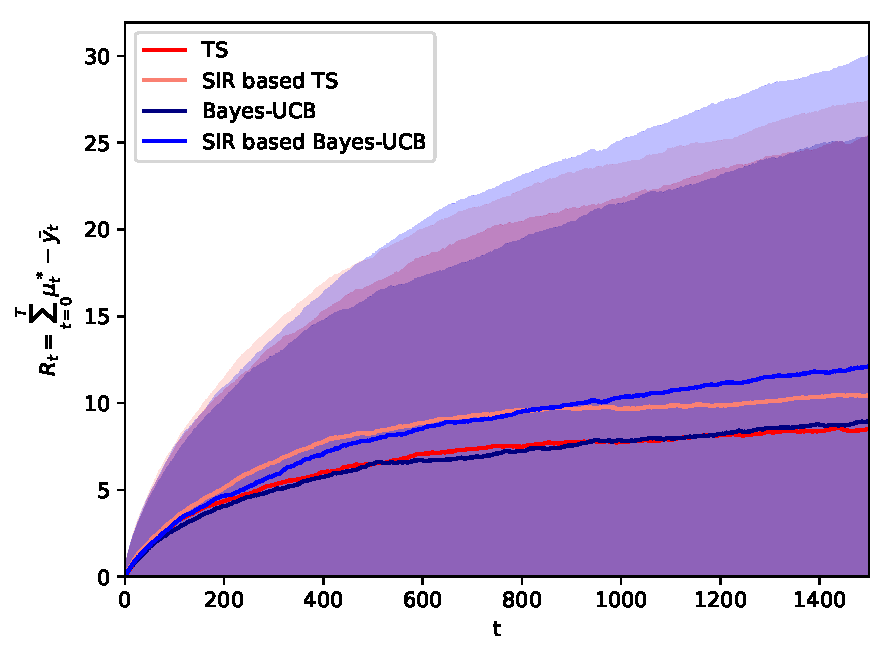
\includegraphics[width=\textwidth]{./figs_appendix/static/bernoulli/A2/cumulative_regret_01_02}
		\caption{Bernoulli bandit, $\theta_0=0.1,\theta_1=0.2$.}
	\end{subfigure}
	\begin{subfigure}[b]{0.49\textwidth}
		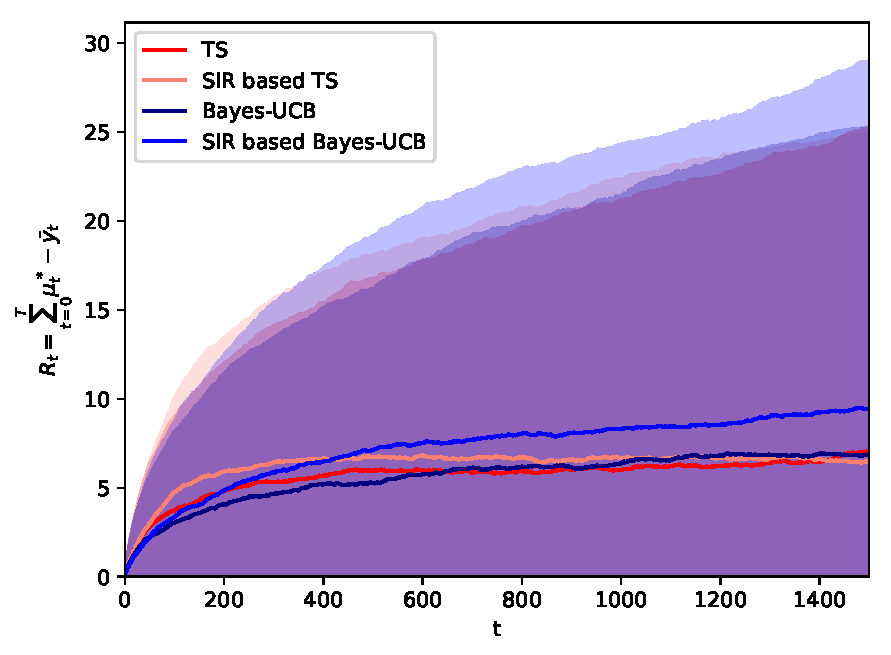
\includegraphics[width=\textwidth]{./figs_appendix/static/bernoulli/A2/cumulative_regret_01_03}
		\caption{Bernoulli bandit, $\theta_0=0.1,\theta_1=0.3$.}
	\end{subfigure}
	
	\begin{subfigure}[b]{0.49\textwidth}
		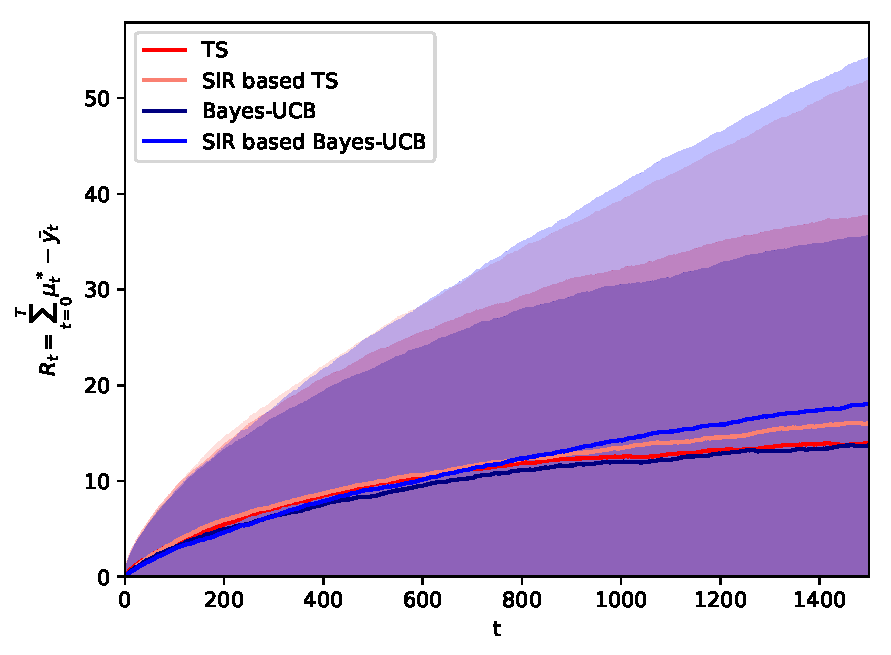
\includegraphics[width=\textwidth]{./figs_appendix/static/bernoulli/A2/cumulative_regret_05_06}
		\caption{Bernoulli bandit, $\theta_0=0.5,\theta_1=0.6$.}
	\end{subfigure}
	\begin{subfigure}[b]{0.49\textwidth}
		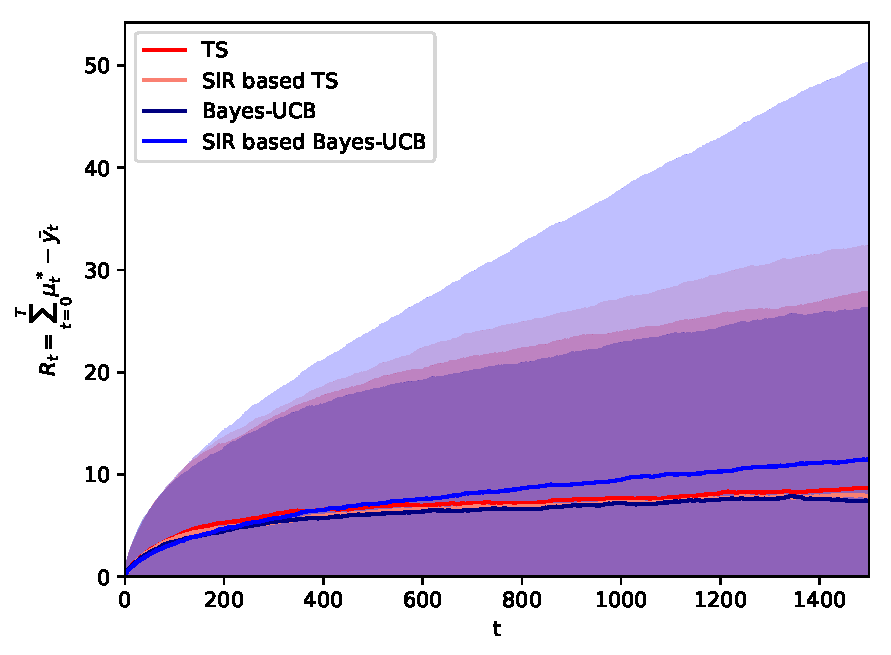
\includegraphics[width=\textwidth]{./figs_appendix/static/bernoulli/A2/cumulative_regret_05_07}
		\caption{Bernoulli bandit, $\theta_0=0.5,\theta_1=0.7$.}
	\end{subfigure}
	
	\begin{subfigure}[b]{0.49\textwidth}
		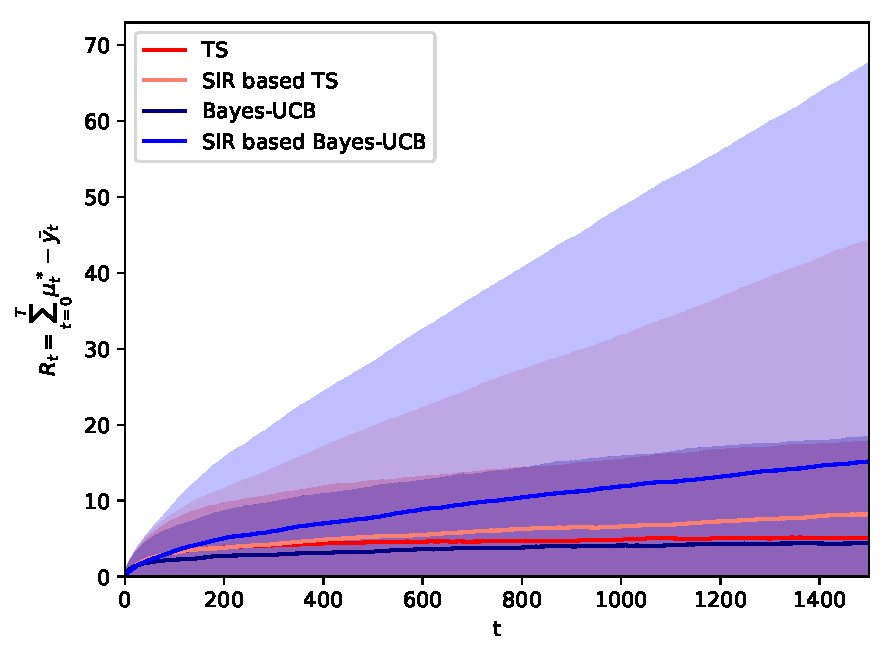
\includegraphics[width=\textwidth]{./figs_appendix/static/bernoulli/A2/cumulative_regret_07_09}
		\caption{Bernoulli bandit, $\theta_0=0.7,\theta_1=0.9$.}
	\end{subfigure}
	\begin{subfigure}[b]{0.49\textwidth}
		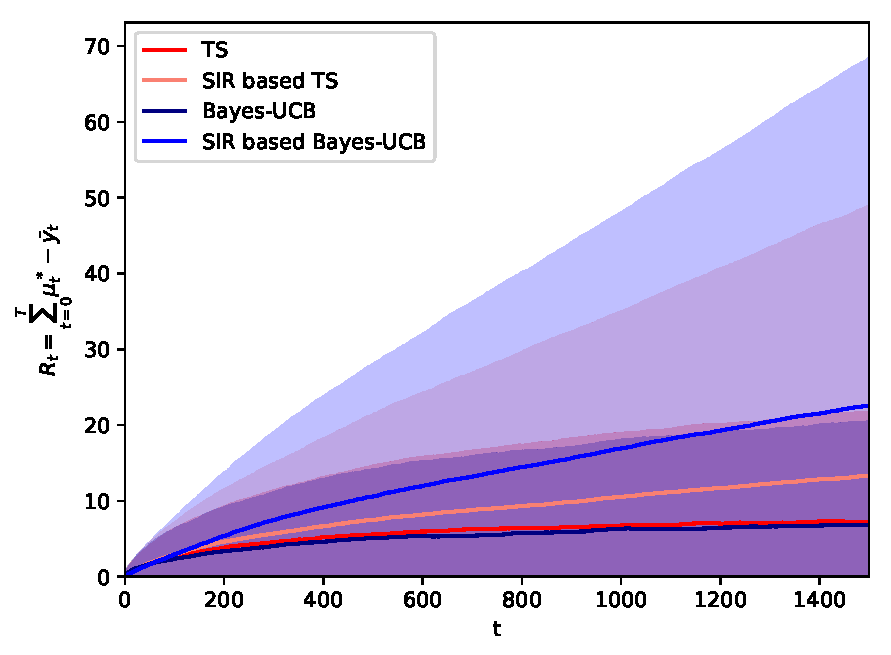
\includegraphics[width=\textwidth]{./figs_appendix/static/bernoulli/A2/cumulative_regret_08_09}
		\caption{Bernoulli bandit, $\theta_0=0.8,\theta_1=0.9$.}
	\end{subfigure}	
	\caption{Mean regret (standard deviation shown as shaded region) in static two-armed Bernoulli bandits.}
\end{figure*}

\clearpage
\begin{figure*}[!h]
	\centering
	\begin{subfigure}[b]{0.49\textwidth}
		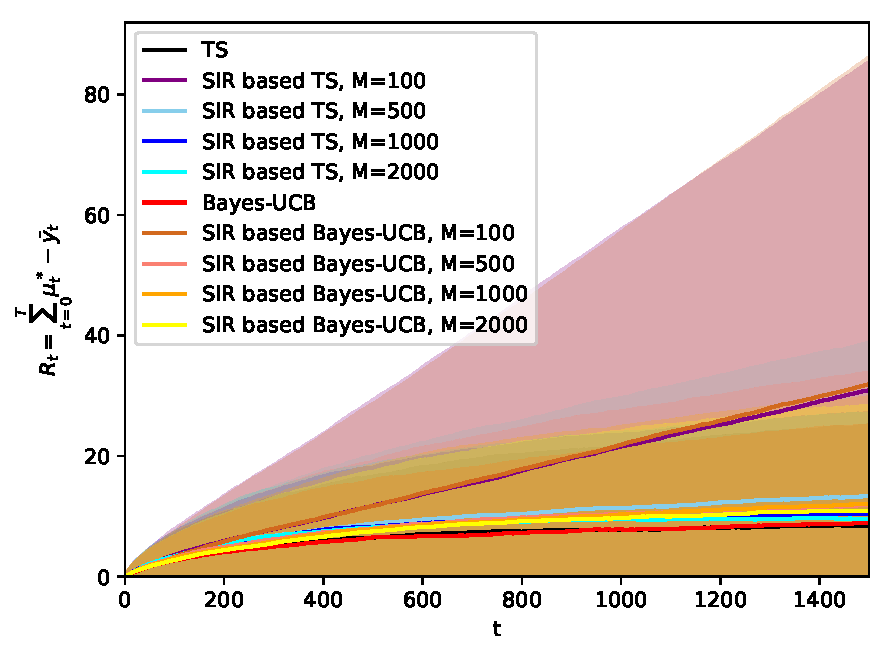
\includegraphics[width=\textwidth]{./figs_appendix/static/bernoulli/A2/cumulative_regret_M_01_02}
		\caption{Bernoulli bandit, $\theta_0=0.1,\theta_1=0.2$.}
	\end{subfigure}
	\begin{subfigure}[b]{0.49\textwidth}
		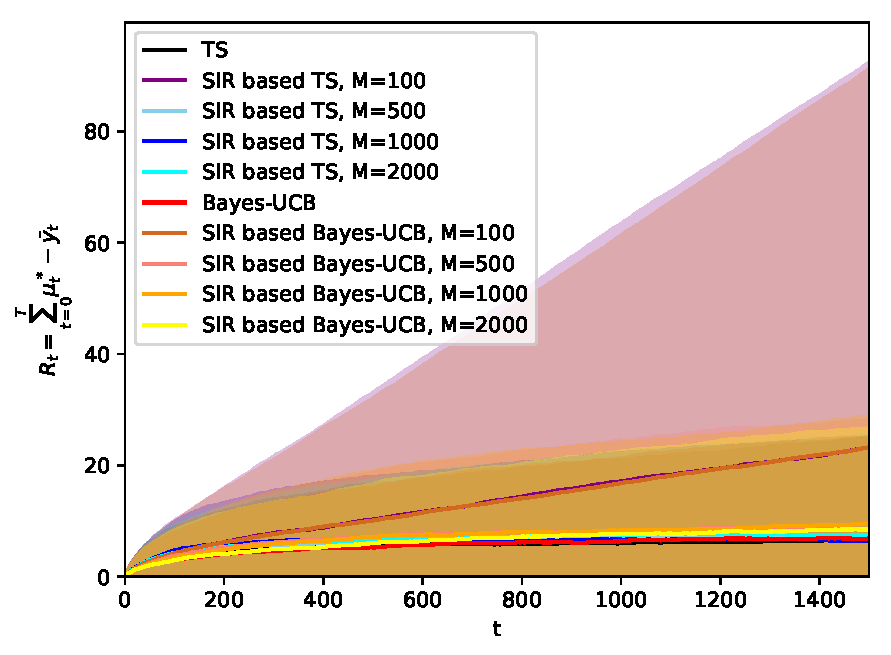
\includegraphics[width=\textwidth]{./figs_appendix/static/bernoulli/A2/cumulative_regret_M_01_03}
		\caption{Bernoulli bandit, $\theta_0=0.1,\theta_1=0.3$.}
	\end{subfigure}
	
	\begin{subfigure}[b]{0.49\textwidth}
		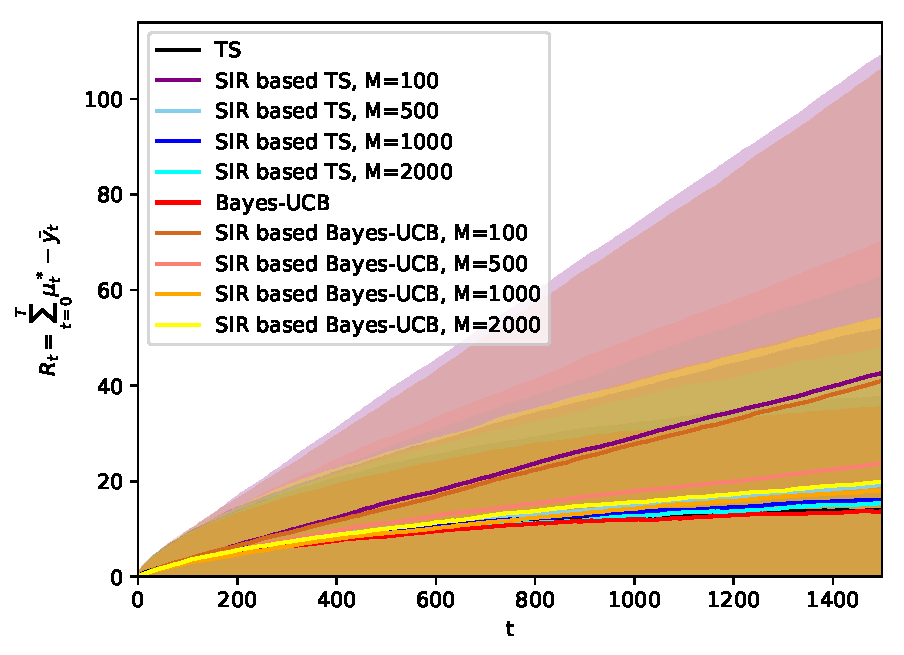
\includegraphics[width=\textwidth]{./figs_appendix/static/bernoulli/A2/cumulative_regret_M_05_06}
		\caption{Bernoulli bandit, $\theta_0=0.5,\theta_1=0.6$.}
	\end{subfigure}
	\begin{subfigure}[b]{0.49\textwidth}
		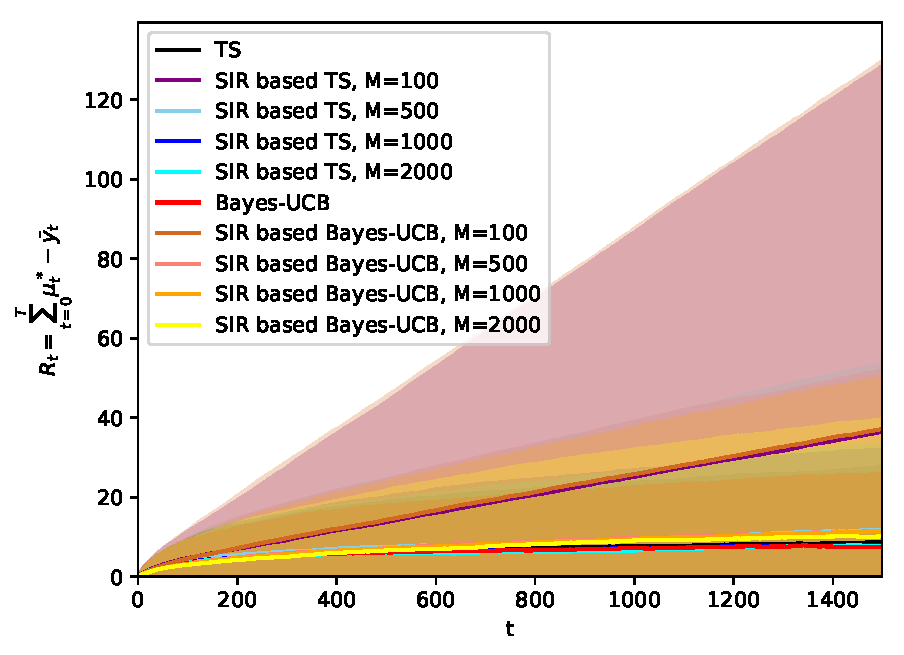
\includegraphics[width=\textwidth]{./figs_appendix/static/bernoulli/A2/cumulative_regret_M_05_07}
		\caption{Bernoulli bandit, $\theta_0=0.5,\theta_1=0.7$.}
	\end{subfigure}
	
	\begin{subfigure}[b]{0.49\textwidth}
		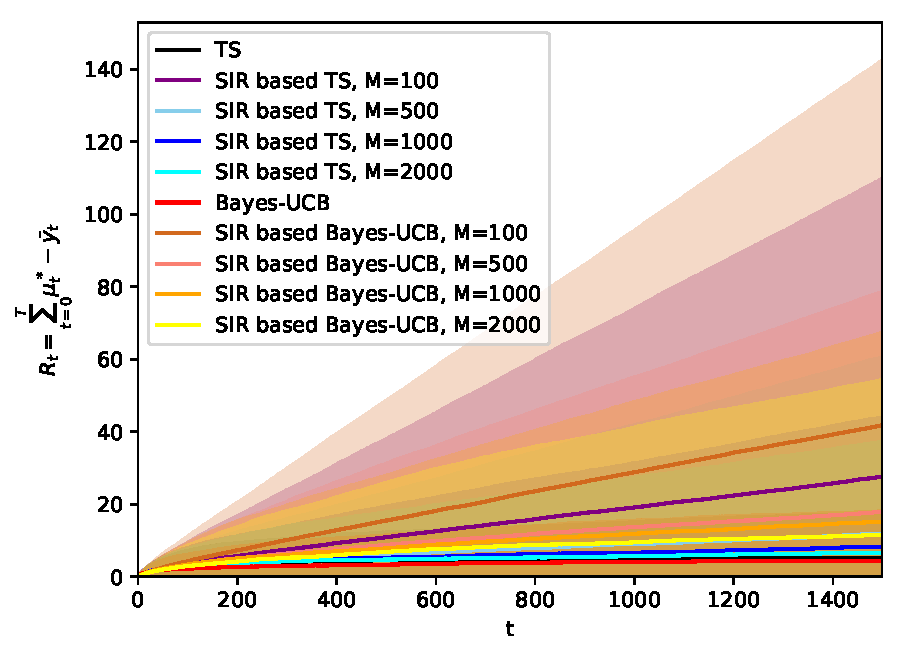
\includegraphics[width=\textwidth]{./figs_appendix/static/bernoulli/A2/cumulative_regret_M_07_09}
		\caption{Bernoulli bandit, $\theta_0=0.7,\theta_1=0.9$.}
	\end{subfigure}
	\begin{subfigure}[b]{0.49\textwidth}
		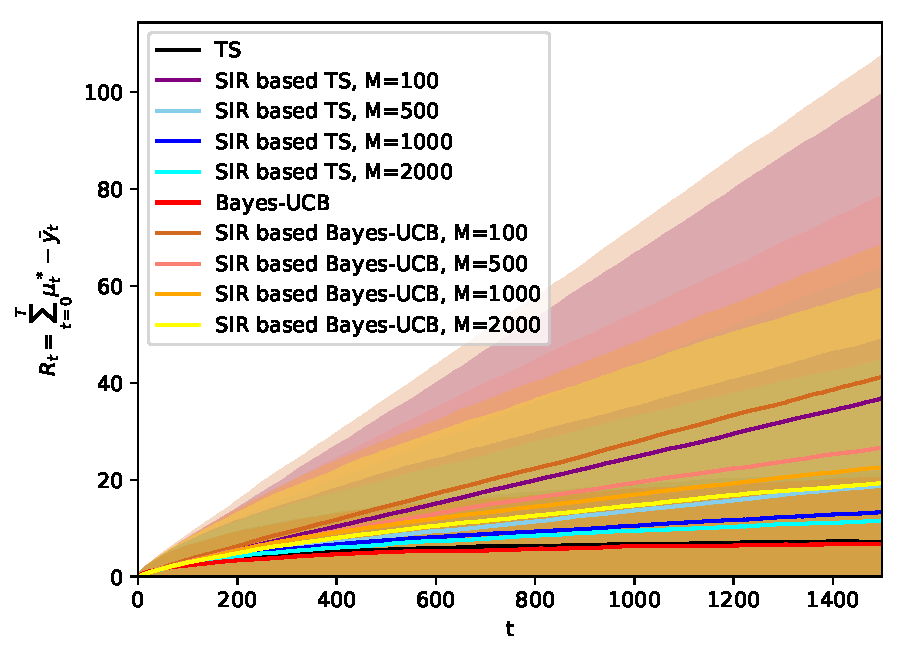
\includegraphics[width=\textwidth]{./figs_appendix/static/bernoulli/A2/cumulative_regret_M_08_09}
		\caption{Bernoulli bandit, $\theta_0=0.8,\theta_1=0.9$.}
	\end{subfigure}	
	\caption{Mean regret (standard deviation shown as shaded region) in static two-armed Bernoulli bandits.}
\end{figure*}

\clearpage

\subsection{Bernoulli bandits, A=3}
\label{assec:statc_bandits_bernoulli_3}

\begin{figure*}[!h]
	\centering
	\begin{subfigure}[b]{0.49\textwidth}
		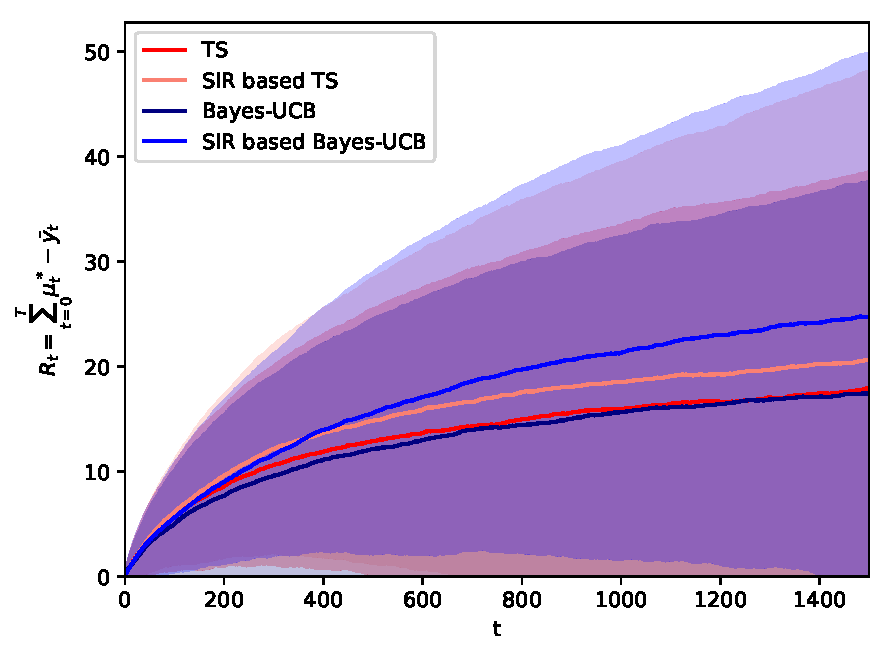
\includegraphics[width=\textwidth]{./figs_appendix/static/bernoulli/A3/cumulative_regret_01_02_03}
		\caption{Bernoulli bandit, $\theta_0=0.1,\theta_1=0.2,\theta_2=0.3$.}
	\end{subfigure}
	\begin{subfigure}[b]{0.49\textwidth}
		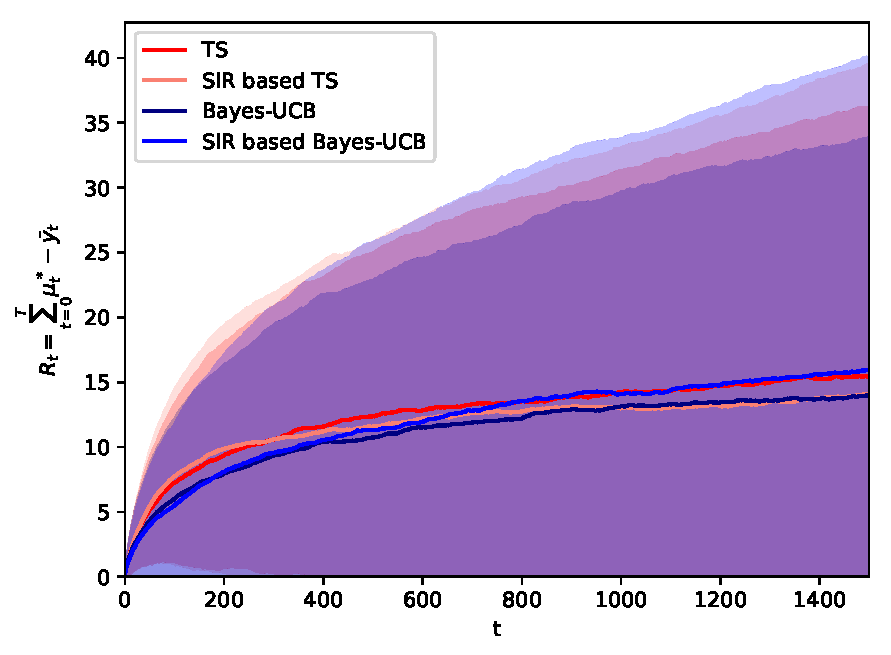
\includegraphics[width=\textwidth]{./figs_appendix/static/bernoulli/A3/cumulative_regret_01_03_05.pdf}
		\caption{Bernoulli bandit, $\theta_0=0.1,\theta_1=0.3,\theta_2=0.5$.}
	\end{subfigure}
	
	\begin{subfigure}[b]{0.49\textwidth}
		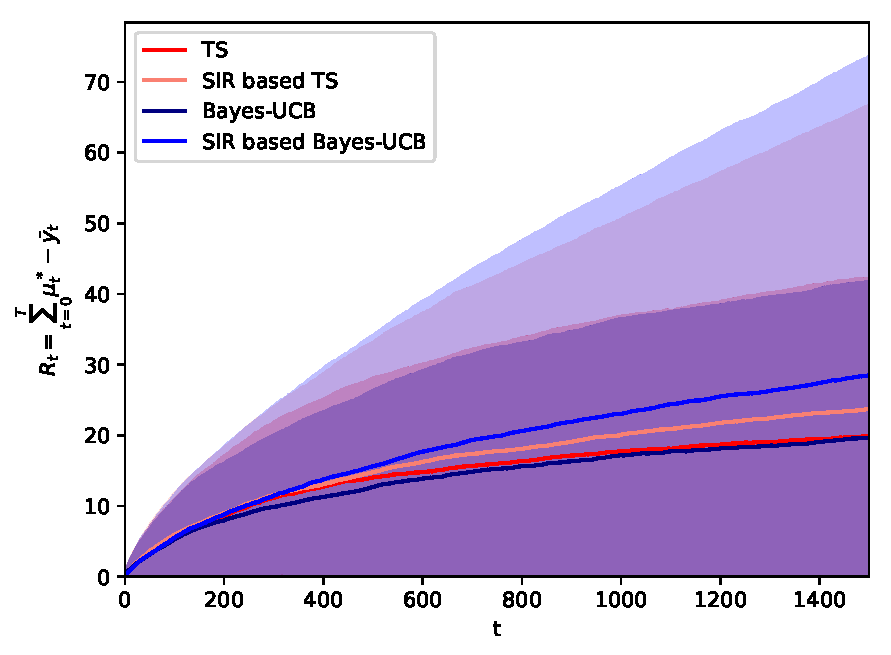
\includegraphics[width=\textwidth]{./figs_appendix/static/bernoulli/A3/cumulative_regret_05_06_07.pdf}
		\caption{Bernoulli bandit, $\theta_0=0.5,\theta_1=0.6,\theta_2=0.7$.}
	\end{subfigure}
	\begin{subfigure}[b]{0.49\textwidth}
		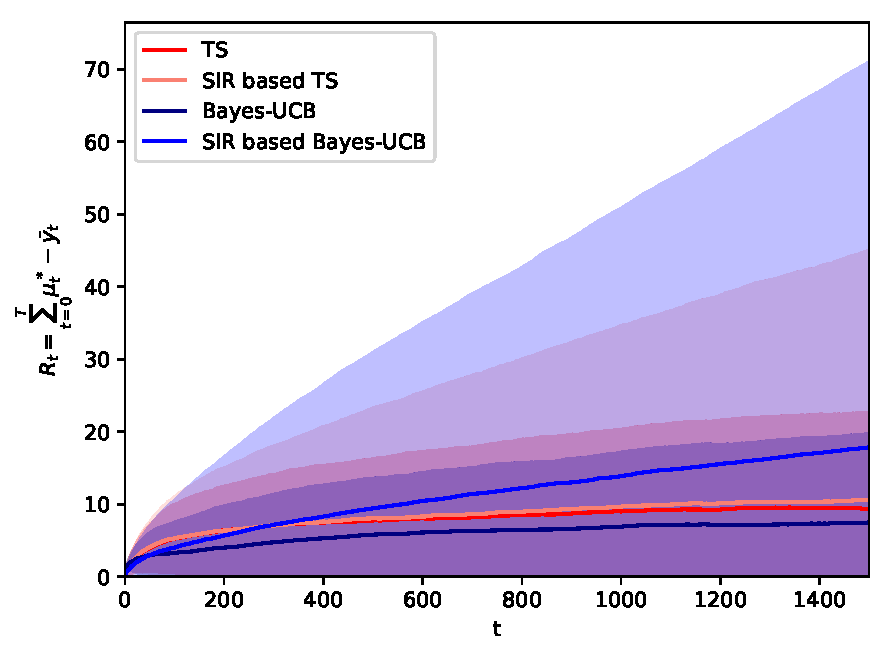
\includegraphics[width=\textwidth]{./figs_appendix/static/bernoulli/A3/cumulative_regret_05_07_09.pdf}
		\caption{Bernoulli bandit, $\theta_0=0.5,\theta_1=0.7,\theta_2=0.9$.}
	\end{subfigure}
	
	\begin{subfigure}[b]{0.49\textwidth}
		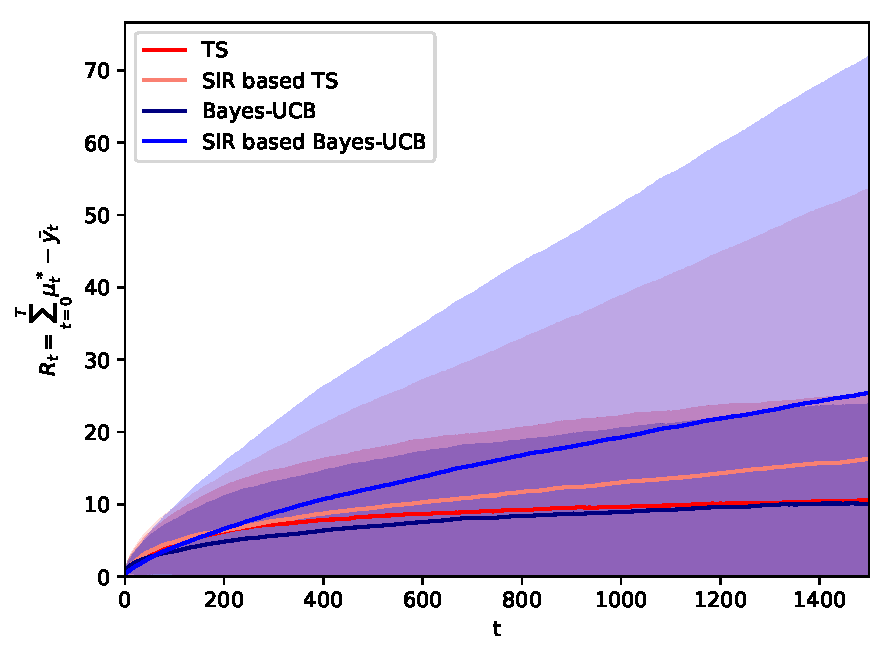
\includegraphics[width=\textwidth]{./figs_appendix/static/bernoulli/A3/cumulative_regret_05_08_09.pdf}
		\caption{Bernoulli bandit, $\theta_0=0.5,\theta_1=0.8,\theta_2=0.9$.}
	\end{subfigure}
	\begin{subfigure}[b]{0.49\textwidth}
		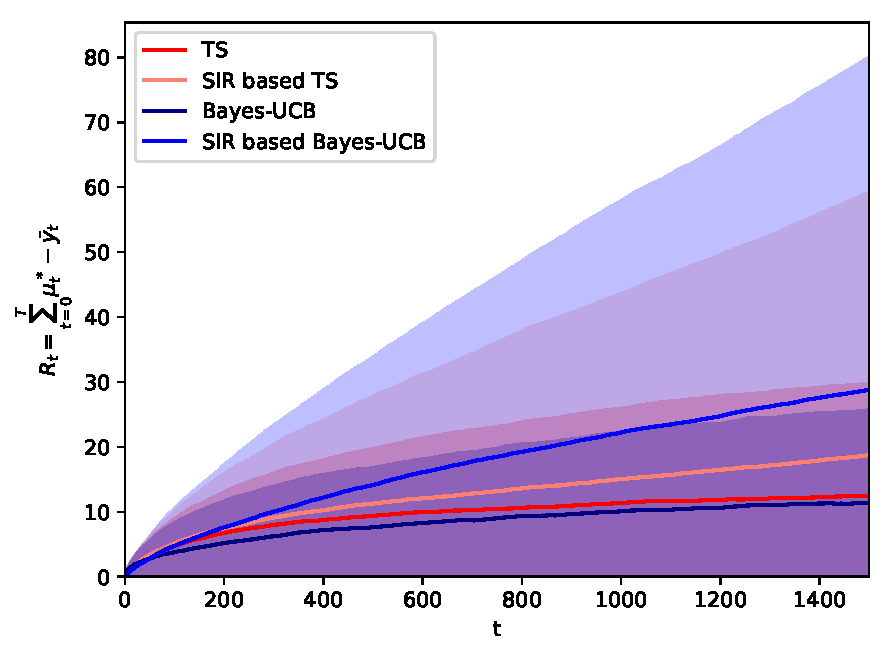
\includegraphics[width=\textwidth]{./figs_appendix/static/bernoulli/A3/cumulative_regret_07_08_09.pdf}
		\caption{Bernoulli bandit, $\theta_0=0.7,\theta_1=0.8,\theta_2=0.9$.}
	\end{subfigure}	
	\caption{Mean regret (standard deviation shown as shaded region) in static three-armed Bernoulli bandits.}
\end{figure*}

\clearpage
\begin{figure*}[!h]
	\centering
	\begin{subfigure}[b]{0.49\textwidth}
		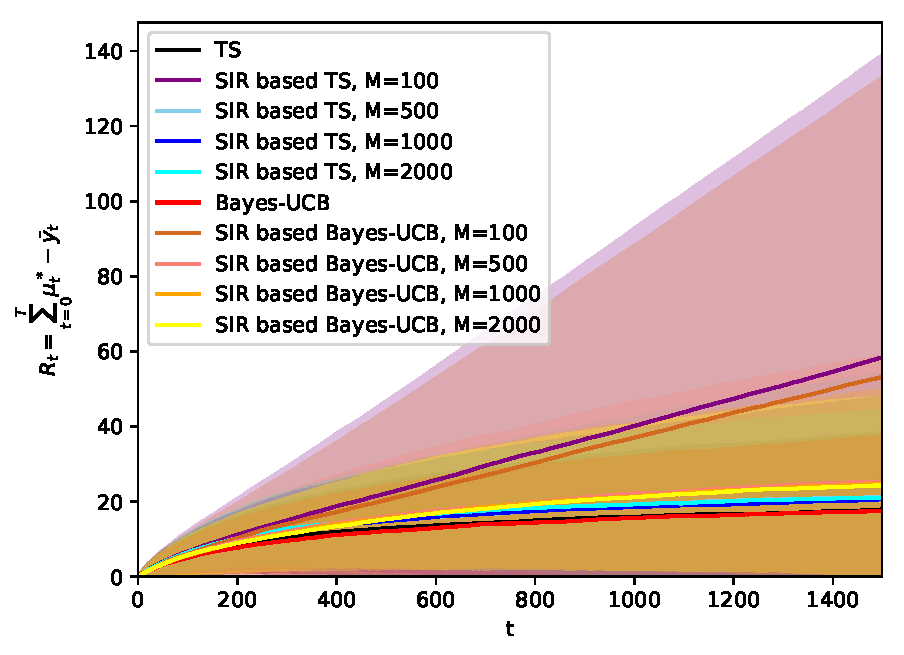
\includegraphics[width=\textwidth]{./figs_appendix/static/bernoulli/A3/cumulative_regret_M_01_02_03.pdf}
		\caption{Bernoulli bandit, $\theta_0=0.1,\theta_1=0.2,\theta_2=0.3$.}
	\end{subfigure}
	\begin{subfigure}[b]{0.49\textwidth}
		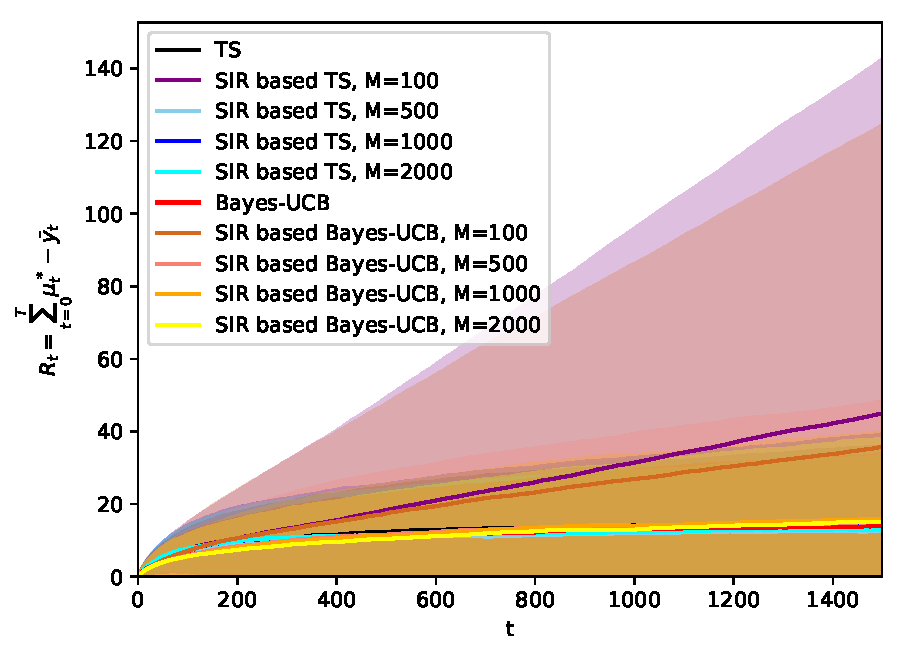
\includegraphics[width=\textwidth]{./figs_appendix/static/bernoulli/A3/cumulative_regret_M_01_03_05.pdf}
		\caption{Bernoulli bandit, $\theta_0=0.1,\theta_1=0.3,\theta_2=0.5$.}
	\end{subfigure}
	
	\begin{subfigure}[b]{0.49\textwidth}
		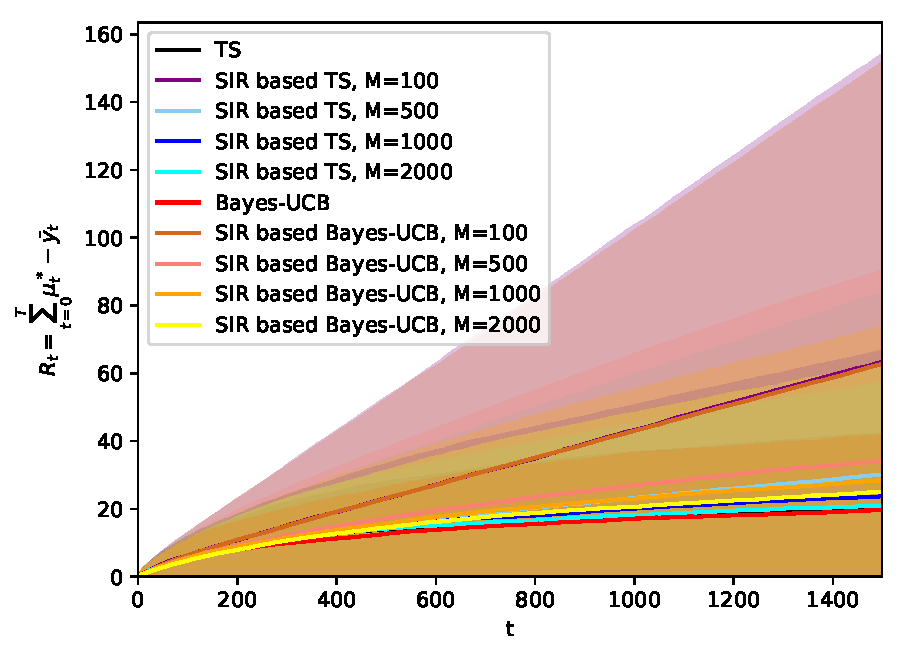
\includegraphics[width=\textwidth]{./figs_appendix/static/bernoulli/A3/cumulative_regret_M_05_06_07.pdf}
		\caption{Bernoulli bandit, $\theta_0=0.5,\theta_1=0.6,\theta_2=0.7$.}
	\end{subfigure}
	\begin{subfigure}[b]{0.49\textwidth}
		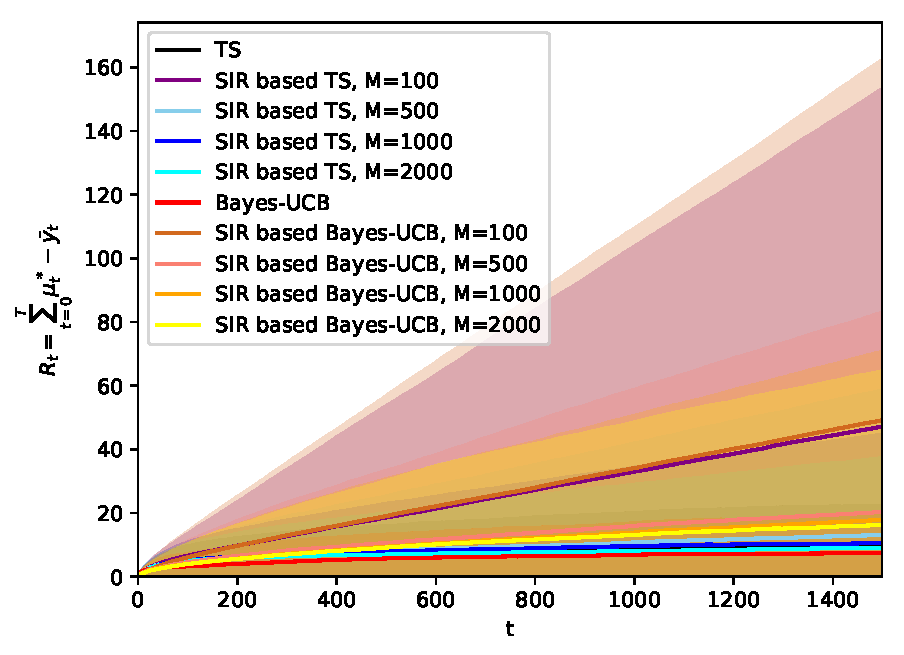
\includegraphics[width=\textwidth]{./figs_appendix/static/bernoulli/A3/cumulative_regret_M_05_07_09.pdf}
		\caption{Bernoulli bandit, $\theta_0=0.5,\theta_1=0.7,\theta_2=0.9$.}
	\end{subfigure}
	
	\begin{subfigure}[b]{0.49\textwidth}
		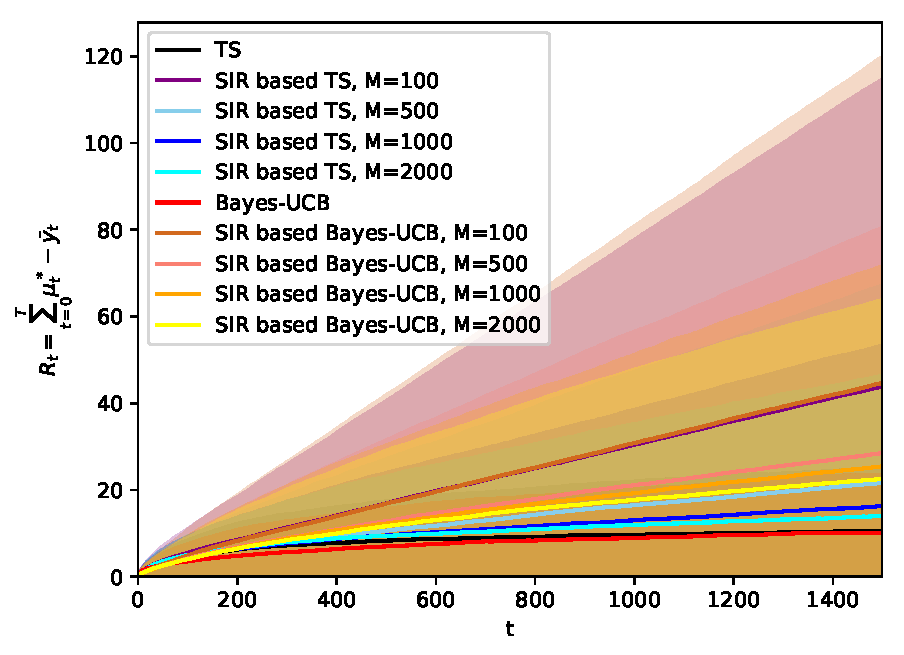
\includegraphics[width=\textwidth]{./figs_appendix/static/bernoulli/A3/cumulative_regret_M_05_08_09.pdf}
		\caption{Bernoulli bandit, $\theta_0=0.5,\theta_1=0.8,\theta_2=0.9$.}
	\end{subfigure}
	\begin{subfigure}[b]{0.49\textwidth}
		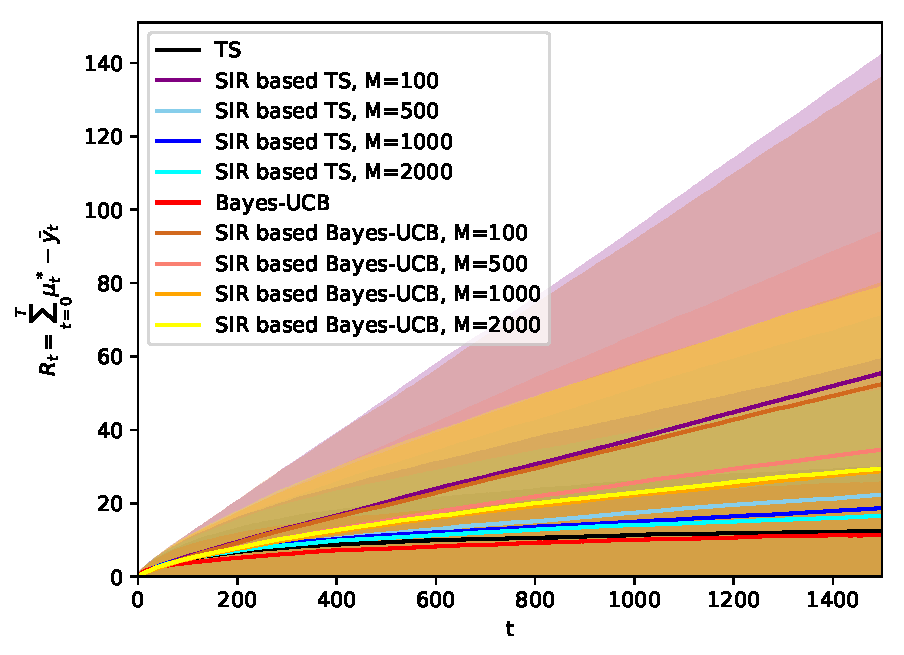
\includegraphics[width=\textwidth]{./figs_appendix/static/bernoulli/A3/cumulative_regret_M_07_08_09.pdf}
		\caption{Bernoulli bandit, $\theta_0=0.7,\theta_1=0.8,\theta_2=0.9$.}
	\end{subfigure}	
	\caption{Mean regret (standard deviation shown as shaded region) in static three-armed Bernoulli bandits.}
\end{figure*}

\clearpage
\subsection{Bernoulli bandits, A=5}
\label{assec:statc_bandits_bernoulli_5}

\begin{figure*}[!h]
	\centering
	\begin{subfigure}[b]{0.45\textwidth}
		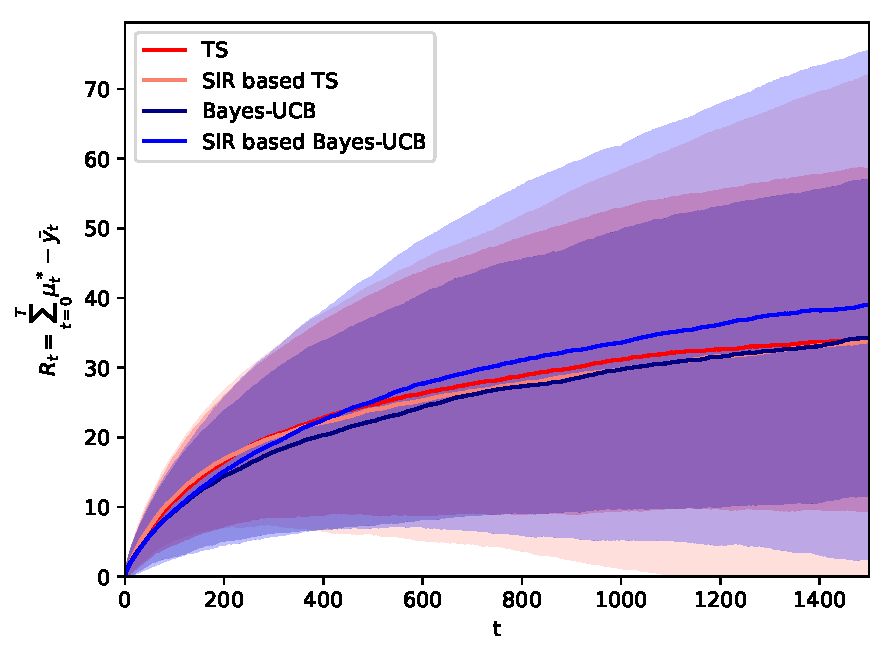
\includegraphics[width=\textwidth]{./figs_appendix/static/bernoulli/A5/cumulative_regret_01_02_03_04_05}
		\caption{Bernoulli bandit, $\theta_0=0.1,\theta_1=0.2,\\ \theta_2=0.3, \theta_3=0.4,\theta_4=0.5$.}
		\end{subfigure}
		\begin{subfigure}[b]{0.45\textwidth}
		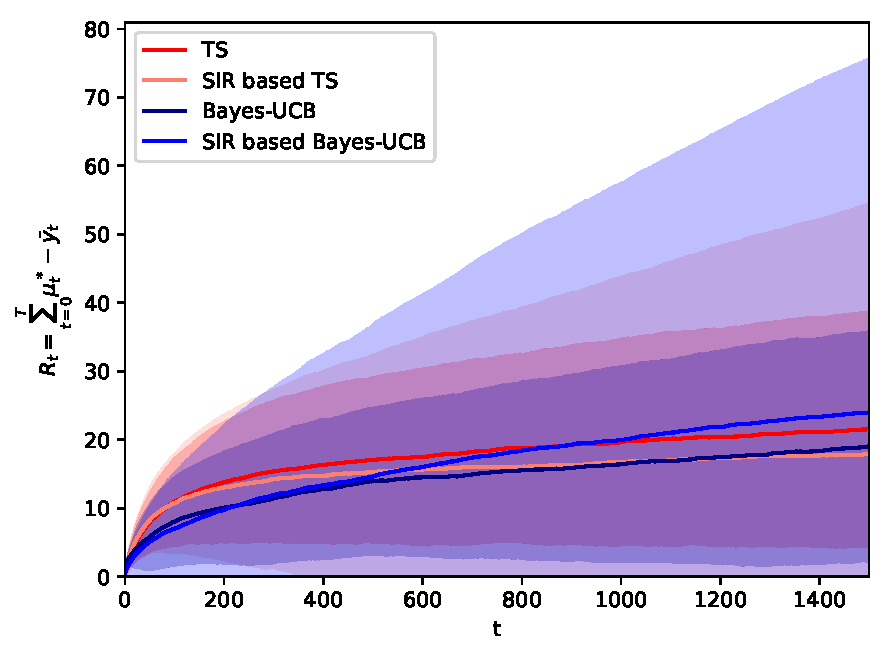
\includegraphics[width=\textwidth]{./figs_appendix/static/bernoulli/A5/cumulative_regret_01_03_05_06_08}
		\caption{Bernoulli bandit, $\theta_0=0.1,\theta_1=0.3,\\ \theta_2=0.5, \theta_3=0.6,\theta_4=0.8$.}
	\end{subfigure}
	
	\begin{subfigure}[b]{0.45\textwidth}
		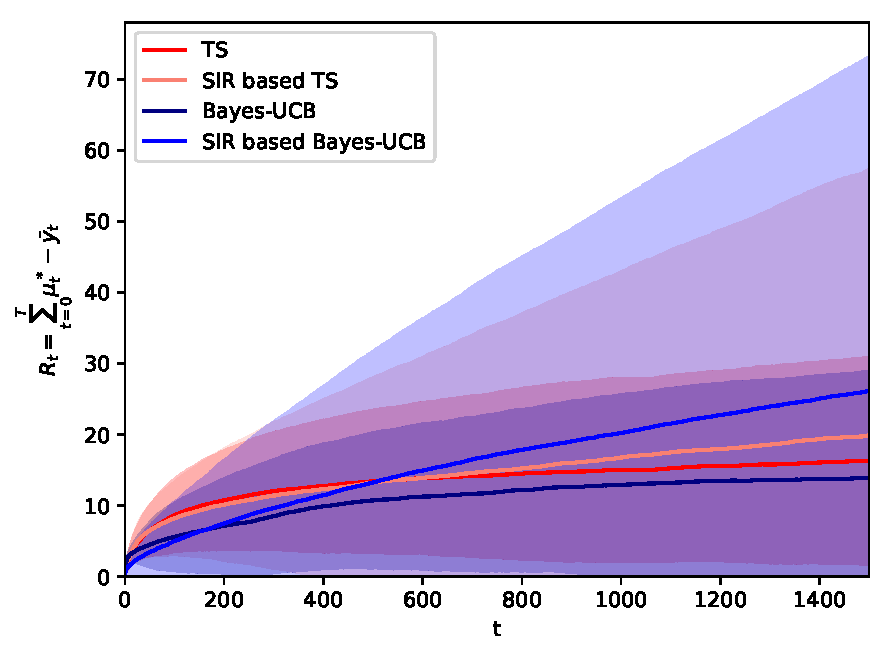
\includegraphics[width=\textwidth]{./figs_appendix/static/bernoulli/A5/cumulative_regret_01_03_05_08_09}
		\caption{Bernoulli bandit, $\theta_0=0.1,\theta_1=0.3, \\ \theta_2=0.5, \theta_3=0.8,\theta_4=0.9$.}
		\end{subfigure}
		\begin{subfigure}[b]{0.45\textwidth}
		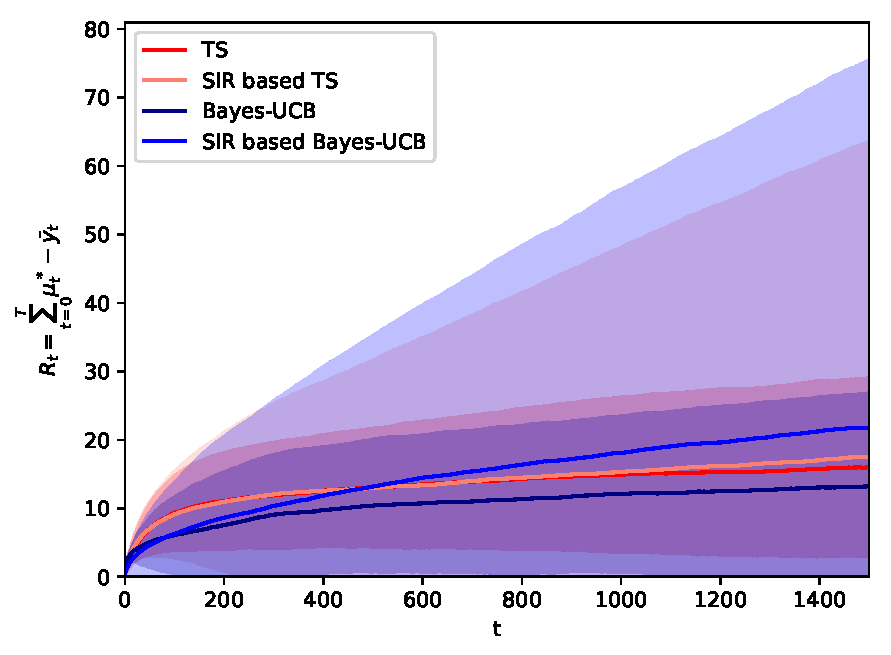
\includegraphics[width=\textwidth]{./figs_appendix/static/bernoulli/A5/cumulative_regret_01_05_06_07_09}
		\caption{Bernoulli bandit, $\theta_0=0.1,\theta_1=0.5,\\ \theta_2=0.6, \theta_3=0.7,\theta_4=0.9$.}
	\end{subfigure}
	
	\begin{subfigure}[b]{0.45\textwidth}
		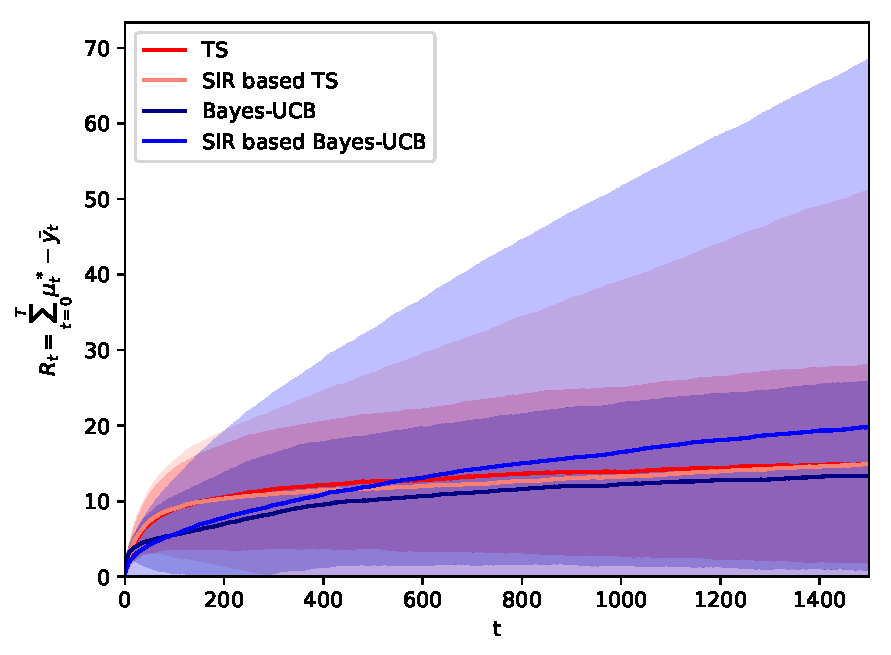
\includegraphics[width=\textwidth]{./figs_appendix/static/bernoulli/A5/cumulative_regret_03_04_05_07_09}
		\caption{Bernoulli bandit, $\theta_0=0.3,\theta_1=0.4,\\ \theta_2=0.5, \theta_3=0.7,\theta_4=0.9$.}
		\end{subfigure}
		\begin{subfigure}[b]{0.45\textwidth}
		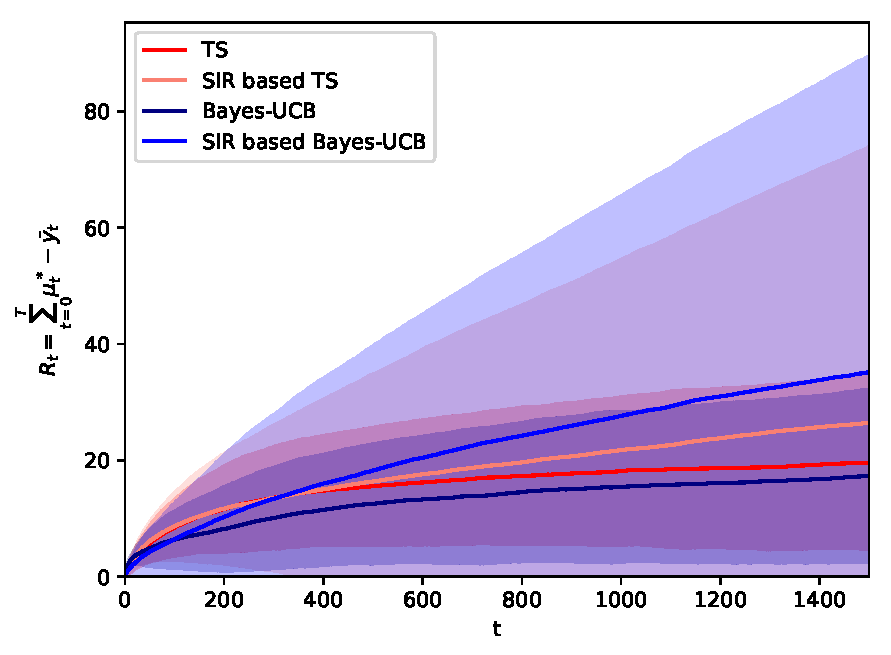
\includegraphics[width=\textwidth]{./figs_appendix/static/bernoulli/A5/cumulative_regret_05_06_07_08_09}
		\caption{Bernoulli bandit, $\theta_0=0.5,\theta_1=0.6,\\ \theta_2=0.7, \theta_3=0.8,\theta_4=0.9$.}
	\end{subfigure}	
	\caption{Mean regret (standard deviation shown as shaded region) in static five-armed Bernoulli bandits.}
\end{figure*}

\clearpage
\begin{figure*}[!h]
	\centering
	\begin{subfigure}[b]{0.49\textwidth}
		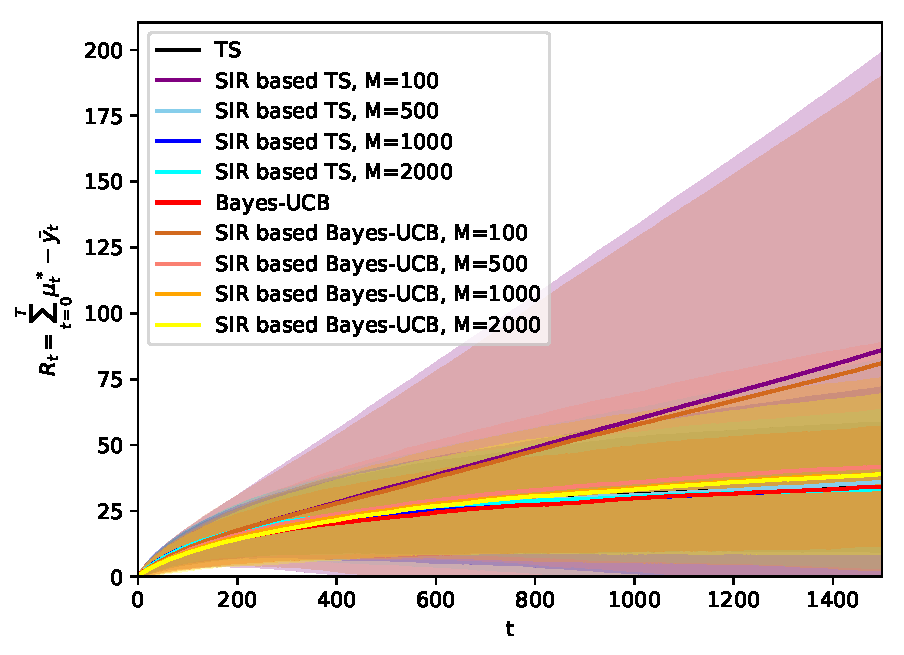
\includegraphics[width=\textwidth]{./figs_appendix/static/bernoulli/A5/cumulative_regret_M_01_02_03_04_05}
		\caption{Bernoulli bandit, $\theta_0=0.1,\theta_1=0.2,\\ \theta_2=0.3, \theta_3=0.4,\theta_4=0.5$.}
		\end{subfigure}
		\begin{subfigure}[b]{0.49\textwidth}
		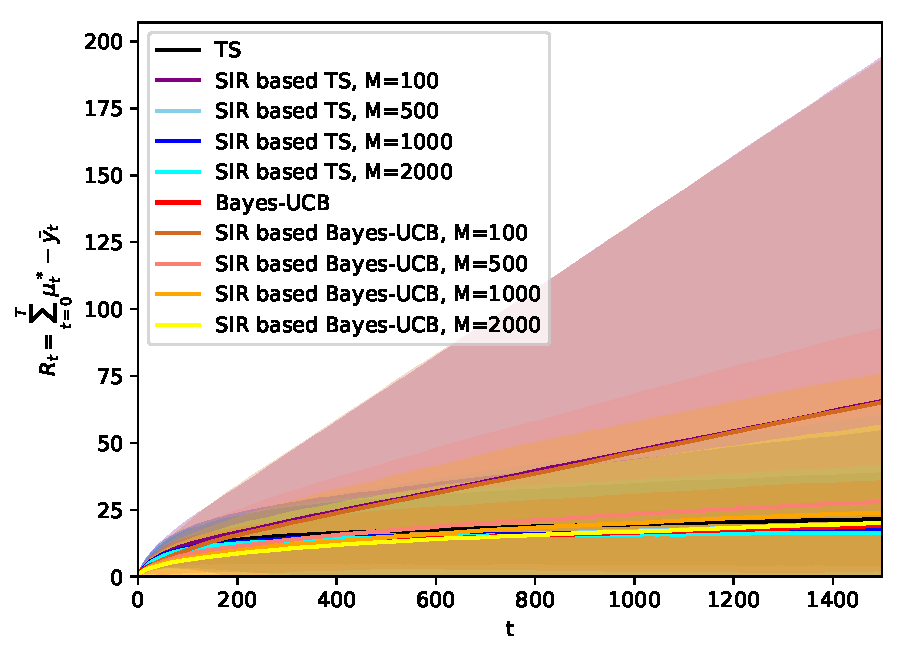
\includegraphics[width=\textwidth]{./figs_appendix/static/bernoulli/A5/cumulative_regret_M_01_03_05_06_08}
		\caption{Bernoulli bandit, $\theta_0=0.1,\theta_1=0.3,\\ \theta_2=0.5, \theta_3=0.6,\theta_4=0.8$.}
	\end{subfigure}
	
	\begin{subfigure}[b]{0.49\textwidth}
		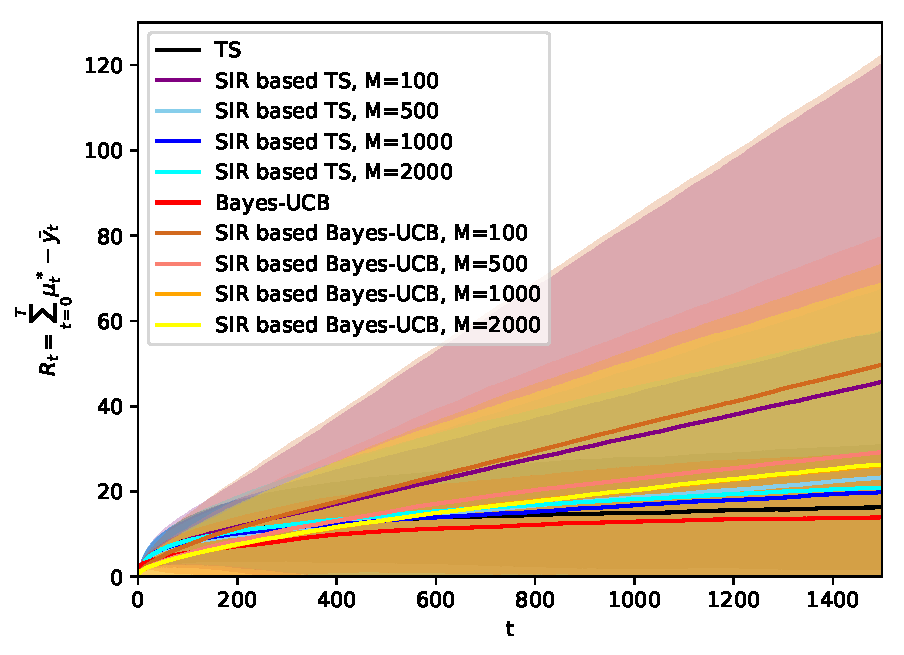
\includegraphics[width=\textwidth]{./figs_appendix/static/bernoulli/A5/cumulative_regret_M_01_03_05_08_09}
		\caption{Bernoulli bandit, $\theta_0=0.1,\theta_1=0.3,\\ \theta_2=0.5, \theta_3=0.8,\theta_4=0.9$.}
		\end{subfigure}
		\begin{subfigure}[b]{0.49\textwidth}
		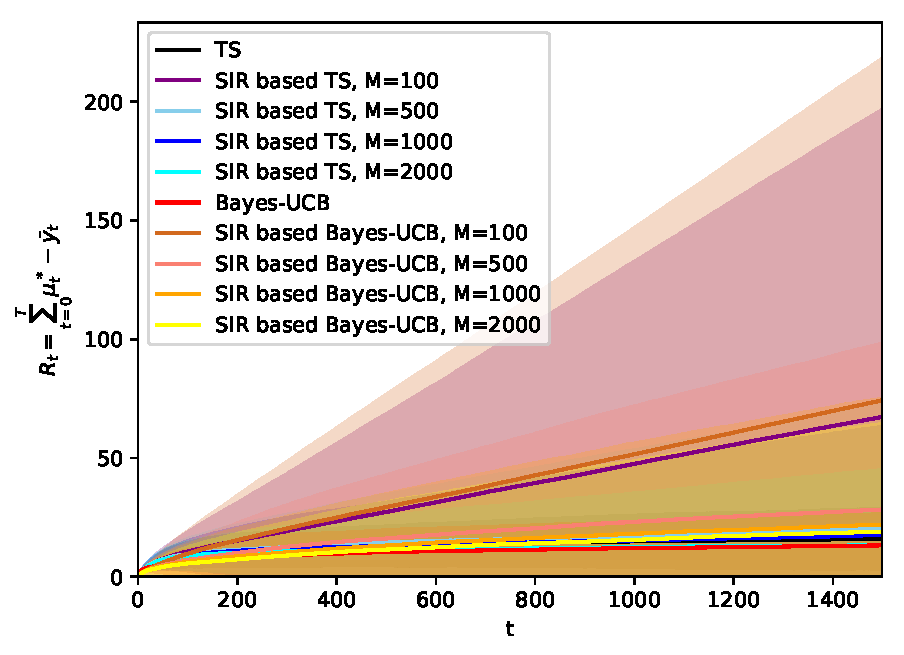
\includegraphics[width=\textwidth]{./figs_appendix/static/bernoulli/A5/cumulative_regret_M_01_05_06_07_09}
		\caption{Bernoulli bandit, $\theta_0=0.1,\theta_1=0.5,\\ \theta_2=0.6, \theta_3=0.7,\theta_4=0.9$.}
	\end{subfigure}
	
	\begin{subfigure}[b]{0.49\textwidth}
		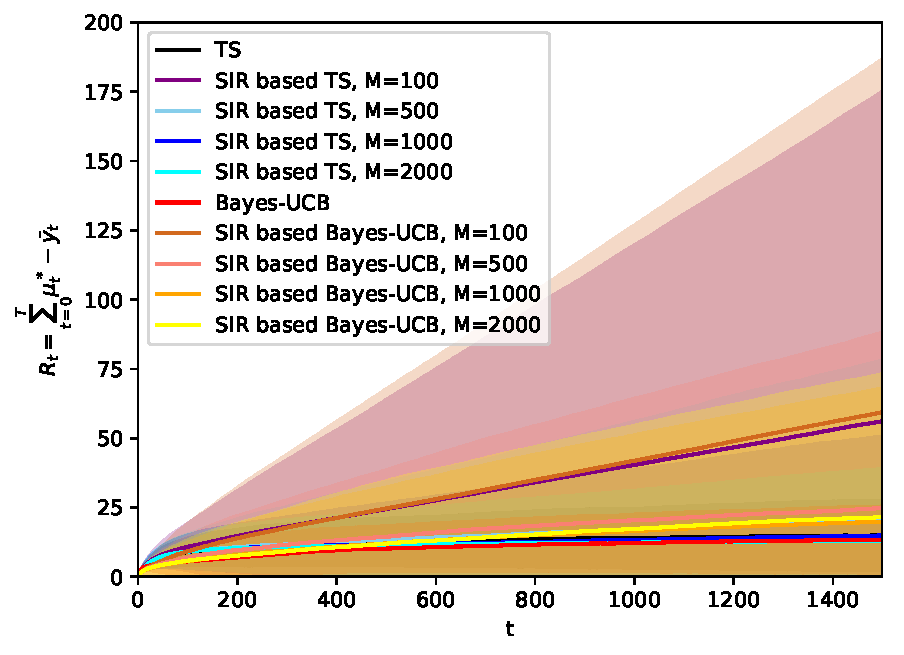
\includegraphics[width=\textwidth]{./figs_appendix/static/bernoulli/A5/cumulative_regret_M_03_04_05_07_09}
		\caption{Bernoulli bandit, $\theta_0=0.3,\theta_1=0.4,\\ \theta_2=0.5, \theta_3=0.7,\theta_4=0.9$.}
		\end{subfigure}
		\begin{subfigure}[b]{0.49\textwidth}
		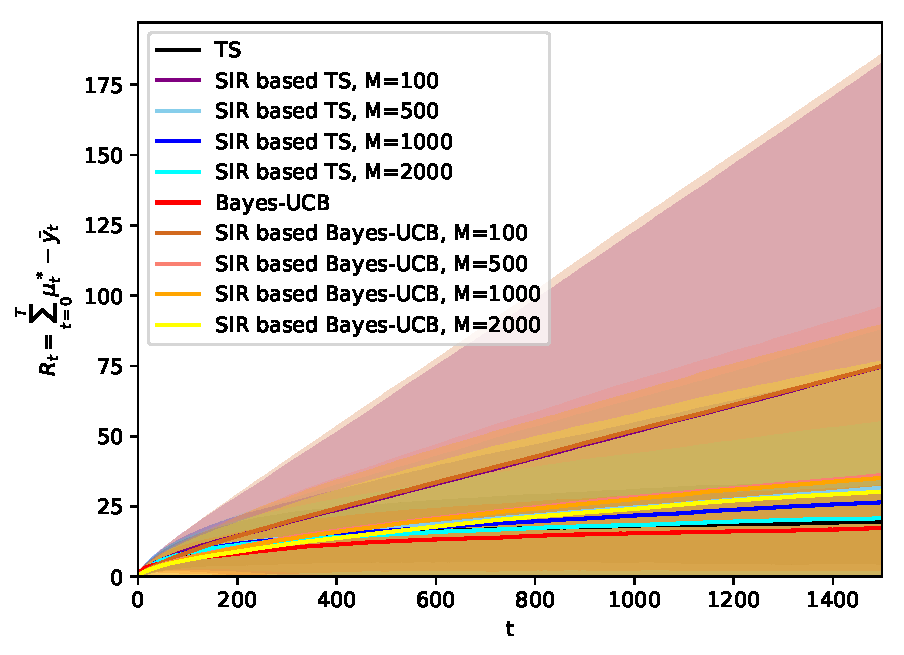
\includegraphics[width=\textwidth]{./figs_appendix/static/bernoulli/A5/cumulative_regret_M_05_06_07_08_09}
		\caption{Bernoulli bandit, $\theta_0=0.5,\theta_1=0.6,\\ \theta_2=0.7, \theta_3=0.8,\theta_4=0.9$.}
	\end{subfigure}	
	\caption{Mean regret (standard deviation shown as shaded region) in static five-armed Bernoulli bandits.}
\end{figure*}

\clearpage

\subsection{Contextual Linear Gaussian bandits, A=2}
\label{assec:statc_bandits_linearGaussian_2}

\begin{figure*}[!h]
	\centering
	\begin{subfigure}[b]{0.35\textwidth}
		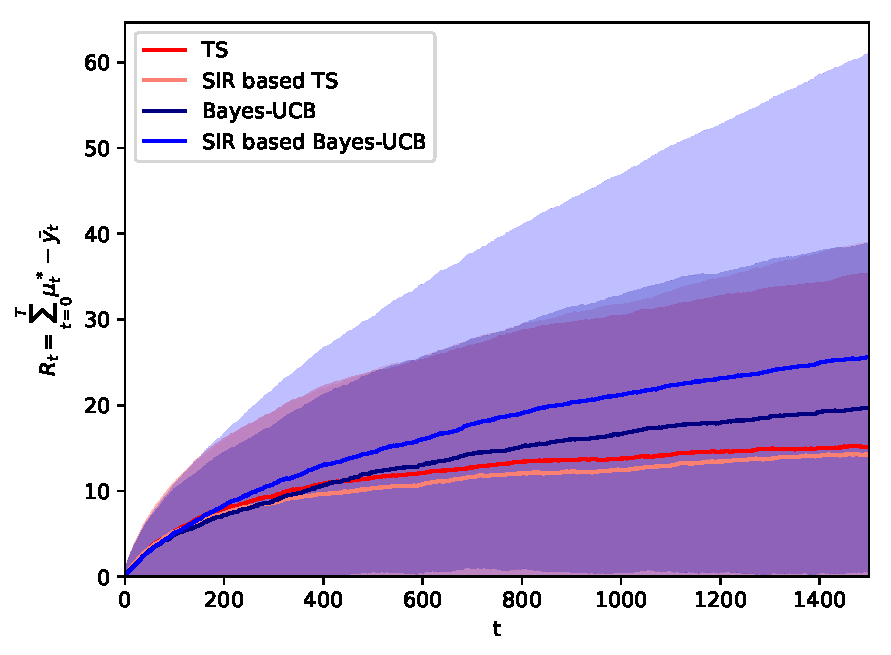
\includegraphics[width=\textwidth]{./figs_appendix/static/linearGaussian/A2/cumulative_regret_known_sigma_-01_-01_01_01_05_05.pdf}
		\caption{Contextual Gaussian bandit, \\ \resizebox{0.95\textwidth}{!}{$\theta_0=(-0.1,-0.1),\theta_1=(0.1,0.1), \sigma^2=0.5$.}}
	\end{subfigure}
	\begin{subfigure}[b]{0.35\textwidth}
		\includegraphics[width=\textwidth]{./figs_appendix/static/linearGaussian/A2/cumulative_regret_known_sigma_-01_-01_01_01_1_1.pdf}
		\caption{Contextual Gaussian bandit, \\ \resizebox{0.95\textwidth}{!}{$\theta_0=(-0.1,-0.1),\theta_1=(0.1,0.1), \sigma^2=1.0$.}}
	\end{subfigure}
	
	\begin{subfigure}[b]{0.35\textwidth}
		\includegraphics[width=\textwidth]{./figs_appendix/static/linearGaussian/A2/cumulative_regret_known_sigma_-05_-05_05_05_05_05.pdf}
		\caption{Contextual Gaussian bandit, \\ \resizebox{0.95\textwidth}{!}{$\theta_0=(-0.5,-0.5),\theta_1=(0.5,0.5), \sigma^2=0.5$.}}
	\end{subfigure}
	\begin{subfigure}[b]{0.35\textwidth}
		\includegraphics[width=\textwidth]{./figs_appendix/static/linearGaussian/A2/cumulative_regret_known_sigma_-05_-05_05_05_1_1.pdf}
		\caption{Contextual Gaussian bandit, \\ \resizebox{0.95\textwidth}{!}{$\theta_0=(-0.5,-0.5),\theta_1=(0.5,0.5), \sigma^2=1.0$.}}
	\end{subfigure}
	
	\begin{subfigure}[b]{0.35\textwidth}
		\includegraphics[width=\textwidth]{./figs_appendix/static/linearGaussian/A2/cumulative_regret_known_sigma_-1_-1_1_1_05_05.pdf}
		\caption{Contextual Gaussian bandit, \\ \resizebox{0.95\textwidth}{!}{$\theta_0=(-1,-1),\theta_1=(1,1), \sigma^2=0.5$.}}
	\end{subfigure}
	\begin{subfigure}[b]{0.35\textwidth}
		\includegraphics[width=\textwidth]{./figs_appendix/static/linearGaussian/A2/cumulative_regret_known_sigma_-1_-1_1_1_1_1.pdf}
		\caption{Contextual Gaussian bandit, \\ \resizebox{0.95\textwidth}{!}{$\theta_0=(-1,-1),\theta_1=(1,1), \sigma^2=1.0$.}}
	\end{subfigure}
	\caption{Mean regret (standard deviation shown as shaded region) in static two-armed contextual Gaussian bandits with reward variance.}
\end{figure*}

\clearpage
\begin{figure*}[!h]
	\centering
	\begin{subfigure}[b]{0.49\textwidth}
		\includegraphics[width=\textwidth]{./figs_appendix/static/linearGaussian/A2/cumulative_regret_all_-01_-01_01_01_05_05.pdf}
		\caption{Contextual Gaussian bandit, \\ \resizebox{0.95\textwidth}{!}{$\theta_0=(-0.1,-0.1),\theta_1=(0.1,0.1), \sigma^2=0.5$.}}
	\end{subfigure}
	\begin{subfigure}[b]{0.49\textwidth}
		\includegraphics[width=\textwidth]{./figs_appendix/static/linearGaussian/A2/cumulative_regret_all_-01_-01_01_01_1_1.pdf}
		\caption{Contextual Gaussian bandit, \\ \resizebox{0.95\textwidth}{!}{$\theta_0=(-0.1,-0.1),\theta_1=(0.1,0.1), \sigma^2=1.0$.}}
	\end{subfigure}
	
	\begin{subfigure}[b]{0.49\textwidth}
		\includegraphics[width=\textwidth]{./figs_appendix/static/linearGaussian/A2/cumulative_regret_all_-05_-05_05_05_05_05.pdf}
		\caption{Contextual Gaussian bandit, \\ \resizebox{0.95\textwidth}{!}{$\theta_0=(-0.5,-0.5),\theta_1=(0.5,0.5), \sigma^2=0.5$.}}
	\end{subfigure}
	\begin{subfigure}[b]{0.49\textwidth}
		\includegraphics[width=\textwidth]{./figs_appendix/static/linearGaussian/A2/cumulative_regret_all_-05_-05_05_05_1_1.pdf}
		\caption{Contextual Gaussian bandit, \\ \resizebox{0.95\textwidth}{!}{$\theta_0=(-0.5,-0.5),\theta_1=(0.5,0.5), \sigma^2=1.0$.}}
	\end{subfigure}
	
	\begin{subfigure}[b]{0.49\textwidth}
		\includegraphics[width=\textwidth]{./figs_appendix/static/linearGaussian/A2/cumulative_regret_all_-1_-1_1_1_05_05.pdf}
		\caption{Contextual Gaussian bandit, \\ \resizebox{0.95\textwidth}{!}{$\theta_0=(-1,-1),\theta_1=(1,1), \sigma^2=0.5$.}}
	\end{subfigure}
	\begin{subfigure}[b]{0.49\textwidth}
		\includegraphics[width=\textwidth]{./figs_appendix/static/linearGaussian/A2/cumulative_regret_all_-1_-1_1_1_1_1.pdf}
		\caption{Contextual Gaussian bandit, \\ \resizebox{0.95\textwidth}{!}{$\theta_0=(-1,-1),\theta_1=(1,1), \sigma^2=1.0$.}}
	\end{subfigure}
	\caption{Mean regret (standard deviation shown as shaded region) in static two-armed contextual Gaussian bandits with unknown reward variance.}
\end{figure*}

\clearpage
\subsection{Contextual Linear Gaussian bandits, A=3}
\label{assec:statc_bandits_linearGaussian_3}

\begin{figure*}[!h]
	\centering
	\begin{subfigure}[b]{0.35\textwidth}
		\includegraphics[width=\textwidth]{./figs_appendix/static/linearGaussian/A3/cumulative_regret_known_sigma_-01_-01_0_0_01_01_05_05_05.pdf}
		\caption{Contextual Gaussian bandit, \\ \resizebox{0.95\textwidth}{!}{$\theta_0=(-0.1,-0.1),\theta_1=(0,0),\theta_2=(0.1,0.1), \sigma^2=0.5$.}}
	\end{subfigure}
	\begin{subfigure}[b]{0.35\textwidth}
		\includegraphics[width=\textwidth]{./figs_appendix/static/linearGaussian/A3/cumulative_regret_known_sigma_-01_-01_0_0_01_01_1_1_1.pdf}
		\caption{Contextual Gaussian bandit, \\ \resizebox{0.95\textwidth}{!}{$\theta_0=(-0.1,-0.1),\theta_1=(0,0),\theta_2=(0.1,0.1), \sigma^2=1.0$.}}
	\end{subfigure}
	
	\begin{subfigure}[b]{0.35\textwidth}
		\includegraphics[width=\textwidth]{./figs_appendix/static/linearGaussian/A3/cumulative_regret_known_sigma_-05_-05_0_0_05_05_05_05_05.pdf}
		\caption{Contextual Gaussian bandit, \\ \resizebox{0.95\textwidth}{!}{$\theta_0=(-0.5,-0.5),\theta_1=(0,0),\theta_2=(0.5,0.5), \sigma^2=0.5$.}}
	\end{subfigure}
	\begin{subfigure}[b]{0.35\textwidth}
		\includegraphics[width=\textwidth]{./figs_appendix/static/linearGaussian/A3/cumulative_regret_known_sigma_-05_-05_0_0_05_05_1_1_1.pdf}
		\caption{Contextual Gaussian bandit, \\ \resizebox{0.95\textwidth}{!}{$\theta_0=(-0.5,-0.5),\theta_1=(0,0),\theta_2=(0.5,0.5), \sigma^2=1.0$.}}
	\end{subfigure}
	
	\begin{subfigure}[b]{0.35\textwidth}
		\includegraphics[width=\textwidth]{./figs_appendix/static/linearGaussian/A3/cumulative_regret_known_sigma_-1_-1_0_0_1_1_05_05_05.pdf}
		\caption{Contextual Gaussian bandit, \\ \resizebox{0.95\textwidth}{!}{$\theta_0=(-1,-1),\theta_1=(0,0),\theta_2=(1,1), \sigma^2=0.5$.}}
	\end{subfigure}
	\begin{subfigure}[b]{0.35\textwidth}
		\includegraphics[width=\textwidth]{./figs_appendix/static/linearGaussian/A3/cumulative_regret_known_sigma_-1_-1_0_0_1_1_1_1_1.pdf}
		\caption{Contextual Gaussian bandit, \\ \resizebox{0.95\textwidth}{!}{$\theta_0=(-1,-1),\theta_1=(0,0),\theta_2=(1,1), \sigma^2=1.0$.}}
	\end{subfigure}
	\caption{Mean regret (standard deviation shown as shaded region) in static three-armed contextual Gaussian bandits with reward variance.}
\end{figure*}

\clearpage
\begin{figure*}[!h]
	\centering
	\begin{subfigure}[b]{0.49\textwidth}
		\includegraphics[width=\textwidth]{./figs_appendix/static/linearGaussian/A3/cumulative_regret_all_-01_-01_0_0_01_01_05_05_05.pdf}
		\caption{Contextual Gaussian bandit, \\ \resizebox{0.95\textwidth}{!}{$\theta_0=(-0.1,-0.1),\theta_1=(0,0),\theta_2=(0.1,0.1), \sigma^2=0.5$.}}
	\end{subfigure}
	\begin{subfigure}[b]{0.49\textwidth}
		\includegraphics[width=\textwidth]{./figs_appendix/static/linearGaussian/A3/cumulative_regret_all_-01_-01_0_0_01_01_1_1_1.pdf}
		\caption{Contextual Gaussian bandit, \\ \resizebox{0.95\textwidth}{!}{$\theta_0=(-0.1,-0.1),\theta_1=(0,0),\theta_2=(0.1,0.1), \sigma^2=1.0$.}}
	\end{subfigure}
	
	\begin{subfigure}[b]{0.49\textwidth}
		\includegraphics[width=\textwidth]{./figs_appendix/static/linearGaussian/A3/cumulative_regret_all_-05_-05_0_0_05_05_05_05_05.pdf}
		\caption{Contextual Gaussian bandit, \\ \resizebox{0.95\textwidth}{!}{$\theta_0=(-0.5,-0.5),\theta_1=(0,0),\theta_2=(0.5,0.5), \sigma^2=0.5$.}}
	\end{subfigure}
	\begin{subfigure}[b]{0.49\textwidth}
		\includegraphics[width=\textwidth]{./figs_appendix/static/linearGaussian/A3/cumulative_regret_all_-05_-05_0_0_05_05_1_1_1.pdf}
		\caption{Contextual Gaussian bandit, \\ \resizebox{0.95\textwidth}{!}{$\theta_0=(-0.5,-0.5),\theta_1=(0,0),\theta_2=(0.5,0.5), \sigma^2=1.0$.}}
	\end{subfigure}
	
	\begin{subfigure}[b]{0.49\textwidth}
		\includegraphics[width=\textwidth]{./figs_appendix/static/linearGaussian/A3/cumulative_regret_all_-1_-1_0_0_1_1_05_05_05.pdf}
		\caption{Contextual Gaussian bandit, \\ \resizebox{0.95\textwidth}{!}{$\theta_0=(-1,-1),\theta_1=(0,0),\theta_2=(1,1), \sigma^2=0.5$.}}
	\end{subfigure}
	\begin{subfigure}[b]{0.49\textwidth}
		\includegraphics[width=\textwidth]{./figs_appendix/static/linearGaussian/A3/cumulative_regret_all_-1_-1_0_0_1_1_1_1_1.pdf}
		\caption{Contextual Gaussian bandit, \\ \resizebox{0.95\textwidth}{!}{$\theta_0=(-1,-1),\theta_1=(0,0),\theta_2=(1,1), \sigma^2=1.0$.}}
	\end{subfigure}
	\caption{Mean regret (standard deviation shown as shaded region) in static three-armed contextual Gaussian bandits with unknown reward variance.}
\end{figure*}

\clearpage

\subsection{Contextual Linear Gaussian bandits, A=5}
\label{assec:statc_bandits_linearGaussian_5}

\begin{figure*}[!h]
	\centering
	\begin{subfigure}[b]{0.35\textwidth}
		\includegraphics[width=\textwidth]{./figs_appendix/static/linearGaussian/A5/cumulative_regret_known_sigma_-02_-02_-01_-01_0_0_01_01_02_02_05_05_05_05_05.pdf}
		\caption{Contextual Gaussian bandit, \\ \resizebox{0.95\textwidth}{!}{$\theta_0=(-0.2,-0.2),\theta_1=(-0.1,-0.1),\theta_2=(0,0),\theta_3=(0.1,0.1),\theta_4=(0.2,0.2), \sigma^2=0.5$.}}
	\end{subfigure}
	\begin{subfigure}[b]{0.35\textwidth}
		\includegraphics[width=\textwidth]{./figs_appendix/static/linearGaussian/A5/cumulative_regret_known_sigma_-02_-02_-01_-01_0_0_01_01_02_02_1_1_1_1_1.pdf}
		\caption{Contextual Gaussian bandit, \\ \resizebox{0.95\textwidth}{!}{$\theta_0=(-0.2,-0.2),\theta_1=(-0.1,-0.1),\theta_2=(0,0),\theta_3=(0.1,0.1),\theta_4=(0.2,0.2), \sigma^2=1.0$.}}
	\end{subfigure}
	
	\begin{subfigure}[b]{0.35\textwidth}
		\includegraphics[width=\textwidth]{./figs_appendix/static/linearGaussian/A5/cumulative_regret_known_sigma_-1_-1_-05_-05_0_0_05_05_1_1_05_05_05_05_05.pdf}
		\caption{Contextual Gaussian bandit, \\ \resizebox{0.95\textwidth}{!}{$\theta_0=(-1.0,-1.0),\theta_1=(-0.5,-0.5),\theta_2=(0,0),\theta_3=(0.5,0.5),\theta_4=(1.0,1.0), \sigma^2=0.5$.}}
	\end{subfigure}
	\begin{subfigure}[b]{0.35\textwidth}
		\includegraphics[width=\textwidth]{./figs_appendix/static/linearGaussian/A5/cumulative_regret_known_sigma_-1_-1_-05_-05_0_0_05_05_1_1_1_1_1_1_1.pdf}
		\caption{Contextual Gaussian bandit, \\ \resizebox{0.95\textwidth}{!}{$\theta_0=(-1.0,-1.0),\theta_1=(-0.5,-0.5),\theta_2=(0,0),\theta_3=(0.5,0.5),\theta_4=(1.0,1.0), \sigma^2=1.0$.}}
	\end{subfigure}
	
	\begin{subfigure}[b]{0.35\textwidth}
		\includegraphics[width=\textwidth]{./figs_appendix/static/linearGaussian/A5/cumulative_regret_known_sigma_-2_-2_-1_-1_0_0_1_1_2_2_05_05_05_05_05.pdf}
		\caption{Contextual Gaussian bandit, \\ \resizebox{0.95\textwidth}{!}{$\theta_0=(-2,-2),\theta_1=(-1,-1),\theta_2=(0,0),\theta_3=(1,1),\theta_4=(2,2), \sigma^2=0.5$.}}
	\end{subfigure}
	\begin{subfigure}[b]{0.35\textwidth}
		\includegraphics[width=\textwidth]{./figs_appendix/static/linearGaussian/A5/cumulative_regret_known_sigma_-2_-2_-1_-1_0_0_1_1_2_2_1_1_1_1_1.pdf}
		\caption{Contextual Gaussian bandit, \\ \resizebox{0.95\textwidth}{!}{$\theta_0=(-2,-2),\theta_1=(-1,-1),\theta_2=(0,0),\theta_3=(1,1),\theta_4=(2,2), \sigma^2=1.0$.}}
	\end{subfigure}
	\caption{Mean regret (standard deviation shown as shaded region) in static five-armed contextual Gaussian bandits with reward variance.}
\end{figure*}

\clearpage
\begin{figure*}[!h]
	\centering
	\begin{subfigure}[b]{0.49\textwidth}
		\includegraphics[width=\textwidth]{./figs_appendix/static/linearGaussian/A5/cumulative_regret_all_-02_-02_-01_-01_0_0_01_01_02_02_05_05_05_05_05.pdf}
		\caption{Contextual Gaussian bandit, \\ \resizebox{0.95\textwidth}{!}{$\theta_0=(-0.2,-0.2),\theta_1=(-0.1,-0.1),\theta_2=(0,0),\theta_3=(0.1,0.1),\theta_4=(0.2,0.2), \sigma^2=0.5$.}}
	\end{subfigure}
	\begin{subfigure}[b]{0.49\textwidth}
		\includegraphics[width=\textwidth]{./figs_appendix/static/linearGaussian/A5/cumulative_regret_all_-02_-02_-01_-01_0_0_01_01_02_02_1_1_1_1_1.pdf}
		\caption{Contextual Gaussian bandit, \\ \resizebox{0.95\textwidth}{!}{$\theta_0=(-0.2,-0.2),\theta_1=(-0.1,-0.1),\theta_2=(0,0),\theta_3=(0.1,0.1),\theta_4=(0.2,0.2), \sigma^2=1.0$.}}
	\end{subfigure}
	
	\begin{subfigure}[b]{0.49\textwidth}
		\includegraphics[width=\textwidth]{./figs_appendix/static/linearGaussian/A5/cumulative_regret_all_-1_-1_-05_-05_0_0_05_05_1_1_05_05_05_05_05.pdf}
		\caption{Contextual Gaussian bandit, \\ \resizebox{0.95\textwidth}{!}{$\theta_0=(-1.0,-1.0),\theta_1=(-0.5,-0.5),\theta_2=(0,0),\theta_3=(0.5,0.5),\theta_4=(1.0,1.0), \sigma^2=0.5$.}}
	\end{subfigure}
	\begin{subfigure}[b]{0.49\textwidth}
		\includegraphics[width=\textwidth]{./figs_appendix/static/linearGaussian/A5/cumulative_regret_all_-1_-1_-05_-05_0_0_05_05_1_1_1_1_1_1_1.pdf}
		\caption{Contextual Gaussian bandit, \\ \resizebox{0.95\textwidth}{!}{$\theta_0=(-1.0,-1.0),\theta_1=(-0.5,-0.5),\theta_2=(0,0),\theta_3=(0.5,0.5),\theta_4=(1.0,1.0), \sigma^2=1.0$.}}
	\end{subfigure}
	
	\begin{subfigure}[b]{0.49\textwidth}
		\includegraphics[width=\textwidth]{./figs_appendix/static/linearGaussian/A5/cumulative_regret_all_-2_-2_-1_-1_0_0_1_1_2_2_05_05_05_05_05.pdf}
		\caption{Contextual Gaussian bandit, \\ \resizebox{0.95\textwidth}{!}{$\theta_0=(-2,-2),\theta_1=(-1,-1),\theta_2=(0,0),\theta_3=(1,1),\theta_4=(2,2), \sigma^2=0.5$.}}
	\end{subfigure}
	\begin{subfigure}[b]{0.49\textwidth}
		\includegraphics[width=\textwidth]{./figs_appendix/static/linearGaussian/A5/cumulative_regret_all_-2_-2_-1_-1_0_0_1_1_2_2_1_1_1_1_1.pdf}
		\caption{Contextual Gaussian bandit, \\ \resizebox{0.95\textwidth}{!}{$\theta_0=(-2,-2),\theta_1=(-1,-1),\theta_2=(0,0),\theta_3=(1,1),\theta_4=(2,2), \sigma^2=1.0$.}}
	\end{subfigure}
	\caption{Mean regret (standard deviation shown as shaded region) in static five-armed contextual Gaussian bandits with unknown reward variance.}
\end{figure*}

\clearpage

\subsection{Contextual Logistic bandits, A=2}
\label{assec:statc_bandits_logistic_2}

\begin{figure*}[!h]
	\centering
	\begin{subfigure}[b]{0.35\textwidth}
		\includegraphics[width=\textwidth]{./figs_appendix/static/logistic/A2/cumulative_regret_-01_-01_01_01.pdf}
		\caption{Contextual Logistic bandit, \\ \resizebox{0.95\textwidth}{!}{$\theta_0=(-0.1,-0.1),\theta_1=(0.1,0.1)$.}}
	\end{subfigure}
	\begin{subfigure}[b]{0.35\textwidth}
		\includegraphics[width=\textwidth]{./figs_appendix/static/logistic/A2/cumulative_regret_-01_-01_01_01.pdf}
		\caption{Contextual Logistic bandit, \\ \resizebox{0.95\textwidth}{!}{$\theta_0=(-0.1,-0.1),\theta_1=(0.1,0.1)$.}}
	\end{subfigure}
	
	\begin{subfigure}[b]{0.35\textwidth}
		\includegraphics[width=\textwidth]{./figs_appendix/static/logistic/A2/cumulative_regret_-05_-05_05_05.pdf}
		\caption{Contextual Logistic bandit, \\ \resizebox{0.95\textwidth}{!}{$\theta_0=(-0.5,-0.5),\theta_1=(0.5,0.5)$.}}
	\end{subfigure}
	\begin{subfigure}[b]{0.35\textwidth}
		\includegraphics[width=\textwidth]{./figs_appendix/static/logistic/A2/cumulative_regret_-05_-05_05_05.pdf}
		\caption{Contextual Logistic bandit, \\ \resizebox{0.95\textwidth}{!}{$\theta_0=(-0.5,-0.5),\theta_1=(0.5,0.5)$.}}
	\end{subfigure}
	
	\begin{subfigure}[b]{0.35\textwidth}
		\includegraphics[width=\textwidth]{./figs_appendix/static/logistic/A2/cumulative_regret_-1_-1_1_1.pdf}
		\caption{Contextual Logistic bandit, \\ \resizebox{0.95\textwidth}{!}{$\theta_0=(-1,-1),\theta_1=(1,1)$.}}
	\end{subfigure}
	\begin{subfigure}[b]{0.35\textwidth}
		\includegraphics[width=\textwidth]{./figs_appendix/static/logistic/A2/cumulative_regret_-1_-1_1_1.pdf}
		\caption{Contextual Logistic bandit, \\ \resizebox{0.95\textwidth}{!}{$\theta_0=(-1,-1),\theta_1=(1,1)$.}}
	\end{subfigure}
	\caption{Mean regret (standard deviation shown as shaded region) in static two-armed contextual Logistic bandits.}
\end{figure*}

\clearpage
\subsection{Contextual Logistic bandits, A=3}
\label{assec:statc_bandits_logistic_3}

\begin{figure*}[!h]
	\centering
	\begin{subfigure}[b]{0.35\textwidth}
		\includegraphics[width=\textwidth]{./figs_appendix/static/logistic/A3/cumulative_regret_-01_-01_0_0_01_01.pdf}
		\caption{Contextual Logistic bandit, \\ \resizebox{0.95\textwidth}{!}{$\theta_0=(-0.1,-0.1),\theta_1=(0,0),\theta_2=(0.1,0.1)$.}}
	\end{subfigure}
	\begin{subfigure}[b]{0.35\textwidth}
		\includegraphics[width=\textwidth]{./figs_appendix/static/logistic/A3/cumulative_regret_-01_-01_0_0_01_01.pdf}
		\caption{Contextual Logistic bandit, \\ \resizebox{0.95\textwidth}{!}{$\theta_0=(-0.1,-0.1),\theta_1=(0,0),\theta_2=(0.1,0.1)$.}}
	\end{subfigure}
	
	\begin{subfigure}[b]{0.35\textwidth}
		\includegraphics[width=\textwidth]{./figs_appendix/static/logistic/A3/cumulative_regret_-05_-05_0_0_05_05.pdf}
		\caption{Contextual Logistic bandit, \\ \resizebox{0.95\textwidth}{!}{$\theta_0=(-0.5,-0.5),\theta_1=(0,0),\theta_2=(0.5,0.5)$.}}
	\end{subfigure}
	\begin{subfigure}[b]{0.35\textwidth}
		\includegraphics[width=\textwidth]{./figs_appendix/static/logistic/A3/cumulative_regret_-05_-05_0_0_05_05.pdf}
		\caption{Contextual Logistic bandit, \\ \resizebox{0.95\textwidth}{!}{$\theta_0=(-0.5,-0.5),\theta_1=(0,0),\theta_2=(0.5,0.5)$.}}
	\end{subfigure}
	
	\begin{subfigure}[b]{0.35\textwidth}
		\includegraphics[width=\textwidth]{./figs_appendix/static/logistic/A3/cumulative_regret_-1_-1_0_0_1_1.pdf}
		\caption{Contextual Logistic bandit, \\ \resizebox{0.95\textwidth}{!}{$\theta_0=(-1,-1),\theta_1=(0,0),\theta_2=(1,1)$.}}
	\end{subfigure}
	\begin{subfigure}[b]{0.35\textwidth}
		\includegraphics[width=\textwidth]{./figs_appendix/static/logistic/A3/cumulative_regret_-1_-1_0_0_1_1.pdf}
		\caption{Contextual Logistic bandit, \\ \resizebox{0.95\textwidth}{!}{$\theta_0=(-1,-1),\theta_1=(0,0),\theta_2=(1,1)$.}}
	\end{subfigure}
	\caption{Mean regret (standard deviation shown as shaded region) in static three-armed contextual Logistic bandits.}
\end{figure*}

\clearpage

\subsection{Contextual Logistic bandits, A=5}
\label{assec:statc_bandits_logistic_5}

\begin{figure*}[!h]
	\centering
	\begin{subfigure}[b]{0.35\textwidth}
		\includegraphics[width=\textwidth]{./figs_appendix/static/logistic/A5/cumulative_regret_-02_-02_-01_-01_0_0_01_01_02_02.pdf}
		\caption{Contextual Logistic bandit, \\ \resizebox{0.95\textwidth}{!}{$\theta_0=(-0.2,-0.2),\theta_1=(-0.1,-0.1),\theta_2=(0,0),\theta_3=(0.1,0.1),\theta_4=(0.2,0.2)$.}}
	\end{subfigure}
	\begin{subfigure}[b]{0.35\textwidth}
		\includegraphics[width=\textwidth]{./figs_appendix/static/logistic/A5/cumulative_regret_-02_-02_-01_-01_0_0_01_01_02_02.pdf}
		\caption{Contextual Logistic bandit, \\ \resizebox{0.95\textwidth}{!}{$\theta_0=(-0.2,-0.2),\theta_1=(-0.1,-0.1),\theta_2=(0,0),\theta_3=(0.1,0.1),\theta_4=(0.2,0.2)$.}}
	\end{subfigure}
	
	\begin{subfigure}[b]{0.35\textwidth}
		\includegraphics[width=\textwidth]{./figs_appendix/static/logistic/A5/cumulative_regret_-1_-1_-05_-05_0_0_05_05_1_1.pdf}
		\caption{Contextual Logistic bandit, \\ \resizebox{0.95\textwidth}{!}{$\theta_0=(-1.0,-1.0),\theta_1=(-0.5,-0.5),\theta_2=(0,0),\theta_3=(0.5,0.5),\theta_4=(1.0,1.0)$.}}
	\end{subfigure}
	\begin{subfigure}[b]{0.35\textwidth}
		\includegraphics[width=\textwidth]{./figs_appendix/static/logistic/A5/cumulative_regret_-1_-1_-05_-05_0_0_05_05_1_1.pdf}
		\caption{Contextual Logistic bandit, \\ \resizebox{0.95\textwidth}{!}{$\theta_0=(-1.0,-1.0),\theta_1=(-0.5,-0.5),\theta_2=(0,0),\theta_3=(0.5,0.5),\theta_4=(1.0,1.0)$.}}
	\end{subfigure}
	
	\begin{subfigure}[b]{0.35\textwidth}
		\includegraphics[width=\textwidth]{./figs_appendix/static/logistic/A5/cumulative_regret_-2_-2_-1_-1_0_0_1_1_2_2.pdf}
		\caption{Contextual Logistic bandit, \\ \resizebox{0.95\textwidth}{!}{$\theta_0=(-2,-2),\theta_1=(-1,-1),\theta_2=(0,0),\theta_3=(1,1),\theta_4=(2,2)$.}}
	\end{subfigure}
	\begin{subfigure}[b]{0.35\textwidth}
		\includegraphics[width=\textwidth]{./figs_appendix/static/logistic/A5/cumulative_regret_-2_-2_-1_-1_0_0_1_1_2_2.pdf}
		\caption{Contextual Logistic bandit, \\ \resizebox{0.95\textwidth}{!}{$\theta_0=(-2,-2),\theta_1=(-1,-1),\theta_2=(0,0),\theta_3=(1,1),\theta_4=(2,2)$.}}
	\end{subfigure}
	\caption{Mean regret (standard deviation shown as shaded region) in static five-armed contextual Logistic bandits.}
\end{figure*}

\clearpage
\subsection{Dynamic bandits}
\label{assec:dynamic_bandits}

Fig.~\ref{afig:linear_mixing_dynamics_symmetric_mixing} illustrates the time-evolution of the expected rewards for a realization of the dynamics

\begin{equation}
\begin{split}
\begin{pmatrix}
\theta_{0,0,t}\\
\theta_{0,1,t}\\
\end{pmatrix} &= \begin{pmatrix}
0.9 & -0.1 \\
-0.1 & 0.9 \\
\end{pmatrix} \begin{pmatrix}
\theta_{0,0,t-1}\\
\theta_{0,1,t-1}\\
\end{pmatrix} + \epsilon \; ,\\
\begin{pmatrix}
\theta_{1,0,t}\\
\theta_{1,1,t}\\
\end{pmatrix} &= \begin{pmatrix}
0.9 & 0.1 \\
0.1 & 0.9 \\
\end{pmatrix} \begin{pmatrix}
\theta_{1,0,t-1}\\
\theta_{1,1,t-1}\\
\end{pmatrix} + \epsilon \; ,
\end{split}
\label{aeq:linear_mixing_dynamics_symmetric_mixing}
\end{equation}
and $\epsilon \sim \N{\epsilon|0,0.1 \cdot\mathrm{I}}$. 

\begin{figure}[!h]
	\begin{center}
		\centerline{\includegraphics[width=0.7\columnwidth]{./figs_appendix/dynamic/dynamics_symmetric_mixing}}
		\caption{Expected per-arm rewards over time.}
		\label{afig:linear_mixing_dynamics_symmetric_mixing}
	\end{center}
\end{figure}

Fig.~\ref{afig:linear_mixing_dynamics_noise_mixing} illustrates the time-evolution of the expected rewards for a realization of the dynamics
\begin{equation}
\begin{split}
\begin{pmatrix}
\theta_{0,0,t}\\
\theta_{0,1,t}\\
\end{pmatrix} &= \begin{pmatrix}
0.5 & 0.0 \\
0.0 & 0.5 \\
\end{pmatrix} \begin{pmatrix}
\theta_{0,0,t-1}\\
\theta_{0,1,t-1}\\
\end{pmatrix} + \epsilon \; ,\\
\begin{pmatrix}
\theta_{1,0,t}\\
\theta_{1,1,t}\\
\end{pmatrix} &= \begin{pmatrix}
0.9 & 0.1 \\
0.1 & 0.9 \\
\end{pmatrix} \begin{pmatrix}
\theta_{1,0,t-1}\\
\theta_{1,1,t-1}\\
\end{pmatrix} + \epsilon \; ,
\end{split}
\label{aeq:linear_mixing_dynamics_noise_mixing}
\end{equation}
and $\epsilon \sim \N{\epsilon|0,0.1 \cdot\mathrm{I}}$.

\begin{figure}[!h]
	\begin{center}
		\centerline{\includegraphics[width=0.7\columnwidth]{./figs_appendix/dynamic/dynamics_noise_mixing}}
		\caption{Expected per-arm rewards over time.}
		\label{afig:linear_mixing_dynamics_noise_mixing}
	\end{center}
\end{figure}

Fig.~\ref{afig:linear_mixing_dynamics_no_mixing} illustrates the time-evolution of the expected rewards for a realization of the static dynamics
\begin{equation}
\begin{split}
\begin{pmatrix}
\theta_{0,0,t}\\
\theta_{0,1,t}\\
\end{pmatrix} &= \begin{pmatrix}
1 & 0 \\
0 & 1 \\
\end{pmatrix} \begin{pmatrix}
\theta_{0,0,t-1}\\
\theta_{0,1,t-1}\\
\end{pmatrix} + \epsilon \; ,\\
\begin{pmatrix}
\theta_{1,0,t}\\
\theta_{1,1,t}\\
\end{pmatrix} &= \begin{pmatrix}
1 & 0 \\
0 & 1 \\
\end{pmatrix} \begin{pmatrix}
\theta_{1,0,t-1}\\
\theta_{1,1,t-1}\\
\end{pmatrix} + \epsilon \; ,
\end{split}
\label{aeq:linear_mixing_dynamics_no_mixing}
\end{equation}
and $\epsilon \sim \N{\epsilon|0,0.00001 \cdot\mathrm{I}}$.

\begin{figure}[!h]
	\begin{center}
		\centerline{\includegraphics[width=0.7\columnwidth]{./figs_appendix/dynamic/dynamics_zero_one_separated}}
		\caption{Expected per-arm rewards over time.}
		\label{afig:linear_mixing_dynamics_no_mixing}
	\end{center}
\end{figure}

\clearpage

\begin{figure*}[h]
	\centering
	\begin{subfigure}[b]{0.49\textwidth}
		\includegraphics[width=\textwidth]{./figs_appendix/dynamic/linearGaussian/cumulative_regret_all_dknown_symmetric_mixing_cstatic_sigma1}
		\caption{Contextual logistic bandit with static context and known dynamics.}
	\end{subfigure}
	\begin{subfigure}[b]{0.49\textwidth}
		\includegraphics[width=\textwidth]{./figs_appendix/dynamic/linearGaussian/cumulative_regret_all_dknown_symmetric_mixing_crand_sigma1}
		\caption{Contextual logistic bandit with random context and known dynamics.}
	\end{subfigure}
	\begin{subfigure}[b]{0.49\textwidth}
		\includegraphics[width=\textwidth]{./figs_appendix/dynamic/linearGaussian/cumulative_regret_all_dunknown_symmetric_mixing_cstatic_sigma1}
		\caption{Contextual logistic bandit with static context and known dynamics.}
	\end{subfigure}
	\begin{subfigure}[b]{0.49\textwidth}
		\includegraphics[width=\textwidth]{./figs_appendix/dynamic/linearGaussian/cumulative_regret_all_dunknown_symmetric_mixing_crand_sigma1}
		\caption{Contextual logistic bandit with random context and known dynamics.}
	\end{subfigure}
	\caption{Mean regret (standard deviation shown as shaded region) in dynamic contextual linear-Gaussian bandits with dynamics as in Eqn.~\eqref{aeq:linear_mixing_dynamics_symmetric_mixing}.}
\end{figure*}

\clearpage
\begin{figure*}[h]
	\centering
	\begin{subfigure}[b]{0.49\textwidth}
		\includegraphics[width=\textwidth]{./figs_appendix/dynamic/linearGaussian/cumulative_regret_all_dknown_noise_mixing_cstatic_sigma1}
		\caption{Contextual logistic bandit with static context and known dynamics.}
	\end{subfigure}
	\begin{subfigure}[b]{0.49\textwidth}
		\includegraphics[width=\textwidth]{./figs_appendix/dynamic/linearGaussian/cumulative_regret_all_dknown_noise_mixing_crand_sigma1}
		\caption{Contextual logistic bandit with random context and known dynamics.}
	\end{subfigure}
	\begin{subfigure}[b]{0.49\textwidth}
		\includegraphics[width=\textwidth]{./figs_appendix/dynamic/linearGaussian/cumulative_regret_all_dunknown_noise_mixing_cstatic_sigma1}
		\caption{Contextual logistic bandit with static context and known dynamics.}
	\end{subfigure}
	\begin{subfigure}[b]{0.49\textwidth}
		\includegraphics[width=\textwidth]{./figs_appendix/dynamic/linearGaussian/cumulative_regret_all_dunknown_noise_mixing_crand_sigma1}
		\caption{Contextual logistic bandit with random context and known dynamics.}
	\end{subfigure}
	\caption{Mean regret (standard deviation shown as shaded region) in dynamic contextual linear-Gaussian bandits with dynamics as in Eqn.~\eqref{aeq:linear_mixing_dynamics_noise_mixing}.}
\end{figure*}

\clearpage

\begin{figure*}[h]
	\centering
	\begin{subfigure}[b]{0.49\textwidth}
		\includegraphics[width=\textwidth]{./figs_appendix/dynamic/linearGaussian/cumulative_regret_all_dknown_minusone_one_separated_cstatic_sigma1}
		\caption{Contextual logistic bandit with static context and known dynamics.}
	\end{subfigure}
	\begin{subfigure}[b]{0.49\textwidth}
		\includegraphics[width=\textwidth]{./figs_appendix/dynamic/linearGaussian/cumulative_regret_all_dknown_minusone_one_separated_crand_sigma1}
		\caption{Contextual logistic bandit with random context and known dynamics.}
	\end{subfigure}
	\begin{subfigure}[b]{0.49\textwidth}
		\includegraphics[width=\textwidth]{./figs_appendix/dynamic/linearGaussian/cumulative_regret_all_dunknown_minusone_one_separated_cstatic_sigma1}
		\caption{Contextual logistic bandit with static context and known dynamics.}
	\end{subfigure}
	\begin{subfigure}[b]{0.49\textwidth}
		\includegraphics[width=\textwidth]{./figs_appendix/dynamic/linearGaussian/cumulative_regret_all_dunknown_minusone_one_separated_crand_sigma1}
		\caption{Contextual logistic bandit with random context and known dynamics.}
	\end{subfigure}
	\caption{Mean regret (standard deviation shown as shaded region) in dynamic contextual linear-Gaussian bandits with dynamics as in Eqn.~\eqref{aeq:linear_mixing_dynamics_no_mixing}.}
\end{figure*}

\clearpage

\begin{figure*}[h]
	\centering
	\begin{subfigure}[b]{0.49\textwidth}
		\includegraphics[width=\textwidth]{./figs_appendix/dynamic/logistic/cumulative_regret_all_symmetric_mixing_cstatic}
		\caption{Contextual logistic bandit with static context and dynamics as in Eqn.~\eqref{aeq:linear_mixing_dynamics_symmetric_mixing}.}
	\end{subfigure}
	\begin{subfigure}[b]{0.49\textwidth}
		\includegraphics[width=\textwidth]{./figs_appendix/dynamic/logistic/cumulative_regret_all_symmetric_mixing_crand}
		\caption{Contextual logistic bandit with random context and dynamics as in Eqn.~\eqref{aeq:linear_mixing_dynamics_symmetric_mixing}.}
	\end{subfigure}
	
	\begin{subfigure}[b]{0.49\textwidth}
		\includegraphics[width=\textwidth]{./figs_appendix/dynamic/logistic/cumulative_regret_all_noise_mixing_cstatic}
		\caption{Contextual logistic bandit with static context and dynamics as in Eqn.~\eqref{aeq:linear_mixing_dynamics_noise_mixing}.}
	\end{subfigure}
	\begin{subfigure}[b]{0.49\textwidth}
		\includegraphics[width=\textwidth]{./figs_appendix/dynamic/logistic/cumulative_regret_all_noise_mixing_crand}
		\caption{Contextual logistic bandit with random context and dynamics as in Eqn.~\eqref{aeq:linear_mixing_dynamics_noise_mixing}.}
	\end{subfigure}
	
	\begin{subfigure}[b]{0.49\textwidth}
		\includegraphics[width=\textwidth]{./figs_appendix/dynamic/logistic/cumulative_regret_all_zero_one_separated_cstatic}
		\caption{Contextual logistic bandit with static context and dynamics as in Eqn.~\eqref{aeq:linear_mixing_dynamics_no_mixing}.}
	\end{subfigure}
	\begin{subfigure}[b]{0.49\textwidth}
		\includegraphics[width=\textwidth]{./figs_appendix/dynamic/logistic/cumulative_regret_all_zero_one_separated_crand}
		\caption{Contextual logistic bandit with random context and dynamics as in Eqn.~\eqref{aeq:linear_mixing_dynamics_no_mixing}.}
	\end{subfigure}
	\caption{Mean regret (standard deviation shown as shaded region) in dynamic contextual logistic bandits.}
\end{figure*}

\fi
%%%%%%%%%%%%%%%%%%%%%%%%%%%%%%%%%%%%%%%%%%%%%%%%%%%%%%%%%%%%%%%%%%%%%%%%%%%%%%%

\end{document}
